\documentclass[a4paper,11pt,dvipsnames,twoside,openright]{memoir} 	% Openright aabner kapitler paa hoejresider (openany begge)

%%%% PACKAGES %%%%

% ¤¤ Oversaettelse og tegnsaetning ¤¤ %
\usepackage[utf8]{inputenc}					% Input-indkodning af tegnsaet (UTF8)
\usepackage[english]{babel}					% Dokumentets sprog
\usepackage[T1]{fontenc}					% Output-indkodning af tegnsaet (T1)
\usepackage{lmodern}						% Noget jeg selv har indsat, fordi det ellers ikke virkede
\usepackage{ragged2e,anyfontsize}			% Justering af elementer
%\usepackage{fixltx2e}						% Retter forskellige fejl i LaTeX-kernen
																			
% ¤¤ Figurer og tabeller (floats) ¤¤ %
\usepackage{graphicx} 						% Haandtering af eksterne billeder (JPG, PNG, EPS, PDF)
%\usepackage{eso-pic}						% Tilfoej billedekommandoer paa hver side
\usepackage{wrapfig}						% Indsaettelse af figurer omsvoebt af tekst. \begin{wrapfigure}{Placering}{Stoerrelse}
\usepackage{multirow}                		% Fletning af raekker og kolonner (\multicolumn og \multirow)
\usepackage{multicol}         	        	% Muliggoer output i spalter
\usepackage{rotating}						% Rotation af tekst med \begin{sideways}...\end{sideways}
\usepackage{colortbl} 						% Farver i tabeller (fx \columncolor og \rowcolor)
\usepackage{xcolor}							% Definer farver med \definecolor. Se mere: http://en.wikibooks.org/wiki/LaTeX/Colors
\usepackage{flafter}						% Soerger for at floats ikke optraeder i teksten foer deres reference
\let\newfloat\relax 						% Justering mellem float-pakken og memoir
\usepackage{float}							% Muliggoer eksakt placering af floats, f.eks. \begin{figure}[H]

% ¤¤ Matematik mm. ¤¤
\usepackage{amsmath,amssymb,stmaryrd} 		% Avancerede matematik-udvidelser
\usepackage{mathtools}						% Andre matematik- og tegnudvidelser
\usepackage{textcomp}                 		% Symbol-udvidelser (f.eks. promille-tegn med \textperthousand )
\usepackage{rsphrase}						% Kemi-pakke til RS-saetninger, f.eks. \rsphrase{R1}
\usepackage[version=3]{mhchem} 				% Kemi-pakke til flot og let notation af formler, f.eks. \ce{Fe2O3}
\usepackage{siunitx}						% Flot og konsistent praesentation af tal og enheder med \si{enhed} og \SI{tal}{enhed}
\sisetup{output-decimal-marker = {,}}		% Opsaetning af \SI (DE for komma som decimalseparator) 

% ¤¤ Referencer og kilder ¤¤ %
\usepackage[english]{varioref}				% Muliggoer bl.a. krydshenvisninger med sidetal (\vref)
\usepackage{natbib}
% Udvidelse med naturvidenskabelige citationsmodeller
%\usepackage{xr}							% Referencer til eksternt dokument med \externaldocument{<NAVN>}
%\usepackage{glossaries}					% Terminologi- eller symbolliste (se mere i Daleifs Latex-bog)

%indsat af jeno
\usepackage{paralist}
%indsat af Andreas
%\DeclareUnicodeCharacter{00A0}{~}

% ¤¤ Misc. ¤¤ %
\usepackage{listings}						% Placer kildekode i dokumentet med \begin{lstlisting}...\end{lstlisting}
\usepackage{lipsum}							% Dummy text \lipsum[..]
\usepackage[shortlabels]{enumitem}			% Muliggoer enkelt konfiguration af lister
\usepackage{pdfpages}						% Goer det muligt at inkludere pdf-dokumenter med kommandoen \includepdf[pages={x-y}]{fil.pdf}	
\pdfminorversion=6					% Muliggoer inkludering af pdf dokumenter, af version 1.6 og hoejere - Andreas: Jeg aendrede en gang pdfoptionpdfminorversion -> pdfminorversion, saa hvis noget en gang gaar galt, saa kunne det vaere derfor
\pretolerance=2500 							% Justering af afstand mellem ord (hoejt tal, mindre orddeling og mere luft mellem ord)

% Kommentarer og rettelser med \fxnote. Med 'final' i stedet for 'draft' udloeser hver note en error i den faerdige rapport.
\usepackage[footnote,draft,english,silent,nomargin]{fixme}		


%%%% CUSTOM SETTINGS %%%%

% ¤¤ Marginer ¤¤ %
\setlrmarginsandblock{3.5cm}{2.5cm}{*}		% \setlrmarginsandblock{Indbinding}{Kant}{Ratio}
\setulmarginsandblock{2.5cm}{3.0cm}{*}		% \setulmarginsandblock{Top}{Bund}{Ratio}
\checkandfixthelayout 						% Oversaetter vaerdier til brug for andre pakker

%	¤¤ Afsnitsformatering ¤¤ %
\setlength{\parindent}{0mm}           		% Stoerrelse af indryk
\setlength{\parskip}{3mm}          			% Afstand mellem afsnit ved brug af double Enter
\linespread{1,1}							% Linie afstand

% ¤¤ Litteraturlisten ¤¤ %
\bibpunct[,]{[}{]}{;}{a}{,}{,} 				% Definerer de 6 parametre ved Harvard henvisning (bl.a. parantestype og seperatortegn)
\bibliographystyle{bibtex/harvard}			% Udseende af litteraturlisten.

% ¤¤ Indholdsfortegnelse ¤¤ %
\setsecnumdepth{subsection}		 			% Dybden af nummerede overkrifter (part/chapter/section/subsection)
\maxsecnumdepth{subsection}					% Dokumentklassens graense for nummereringsdybde
\settocdepth{section} 					% Dybden af indholdsfortegnelsen

% ¤¤ Lister ¤¤ %
\setlist{
  topsep=0pt,								% Vertikal afstand mellem tekst og listen
  itemsep=-1ex,								% Vertikal afstand mellem items
} 

% ¤¤ Visuelle referencer ¤¤ %
\usepackage[colorlinks]{hyperref}			% Danner klikbare referencer (hyperlinks) i dokumentet.
\hypersetup{colorlinks = true,				% Opsaetning af farvede hyperlinks (interne links, citeringer og URL)
    linkcolor = black,
    citecolor = black,
    urlcolor = black
}

% ¤¤ Opsaetning af figur- og tabeltekst ¤¤ %
\captionnamefont{\small\bfseries\itshape}	% Opsaetning af tekstdelen ('Figur' eller 'Tabel')
\captiontitlefont{\small}					% Opsaetning af nummerering
\captiondelim{. }							% Seperator mellem nummerering og figurtekst
\hangcaption								% Venstrejusterer flere-liniers figurtekst under hinanden
\captionwidth{\linewidth}					% Bredden af figurteksten
\setlength{\belowcaptionskip}{0pt}			% Afstand under figurteksten
		
% ¤¤ Opsaetning af listings ¤¤ %

\definecolor{commentGreen}{RGB}{34,139,24}
\definecolor{stringPurple}{RGB}{208,76,239}

\lstset{language=Matlab,					% Sprog
	basicstyle=\ttfamily\scriptsize,		% Opsaetning af teksten
	keywords={for,if,while,else,elseif,		% Noegleord at fremhaeve
			  end,break,return,case,
			  switch,function},
	keywordstyle=\color{blue},				% Opsaetning af noegleord
	commentstyle=\color{commentGreen},		% Opsaetning af kommentarer
	stringstyle=\color{stringPurple},		% Opsaetning af strenge
	showstringspaces=false,					% Mellemrum i strenge enten vist eller blanke
	numbers=left, numberstyle=\tiny,		% Linjenumre
	extendedchars=true, 					% Tillader specielle karakterer
	columns=flexible,						% Kolonnejustering
	breaklines, breakatwhitespace=true,		% Bryd lange linjer
}


%This is the code for including Python

\definecolor{maroon}{cmyk}{0, 0.87, 0.68, 0.32}
\definecolor{halfgray}{gray}{0.55}
\definecolor{ipython_frame}{RGB}{207, 207, 207}
\definecolor{ipython_bg}{RGB}{247, 247, 247}
\definecolor{ipython_red}{RGB}{186, 33, 33}
\definecolor{ipython_green}{RGB}{0, 128, 0}
\definecolor{ipython_cyan}{RGB}{64, 128, 128}
\definecolor{ipython_purple}{RGB}{170, 34, 255}

%% Python definition (c) 1998 Michael Weber
%% Additional definitions (2013) Alexis Dimitriadis
%% modified by me (should not have empty lines)
%%
\lstdefinelanguage{iPython}{
    morekeywords={access,and,break,class,continue,def,del,elif,else,except,exec,finally,for,from,global,if,import,in,is,lambda,not,or,pass,print,raise,return,try,while},%
    %
    % Built-ins
    morekeywords=[2]{abs,all,any,basestring,bin,bool,bytearray,callable,chr,classmethod,cmp,compile,complex,delattr,dict,dir,divmod,enumerate,eval,execfile,file,filter,float,format,frozenset,getattr,globals,hasattr,hash,help,hex,id,input,int,isinstance,issubclass,iter,len,list,locals,long,map,max,memoryview,min,next,object,oct,open,ord,pow,property,range,raw_input,reduce,reload,repr,reversed,round,set,setattr,slice,sorted,staticmethod,str,sum,super,tuple,type,unichr,unicode,vars,xrange,zip,apply,buffer,coerce,intern},%
    %
    sensitive=true,%
    morecomment=[l]\#,%
    morestring=[b]',%
    morestring=[b]",%
    %
    morestring=[s]{'''}{'''},% used for documentation text (mulitiline strings)
    morestring=[s]{"""}{"""},% added by Philipp Matthias Hahn
    %
    morestring=[s]{r'}{'},% `raw' strings
    morestring=[s]{r"}{"},%
    morestring=[s]{r'''}{'''},%
    morestring=[s]{r"""}{"""},%
    morestring=[s]{u'}{'},% unicode strings
    morestring=[s]{u"}{"},%
    morestring=[s]{u'''}{'''},%
    morestring=[s]{u"""}{"""},%
    %
    % {replace}{replacement}{lenght of replace}
    % *{-}{-}{1} will not replace in comments and so on
    literate=
    {á}{{\'a}}1 {é}{{\'e}}1 {í}{{\'i}}1 {ó}{{\'o}}1 {ú}{{\'u}}1
    {Á}{{\'A}}1 {É}{{\'E}}1 {Í}{{\'I}}1 {Ó}{{\'O}}1 {Ú}{{\'U}}1
    {à}{{\`a}}1 {è}{{\`e}}1 {ì}{{\`i}}1 {ò}{{\`o}}1 {ù}{{\`u}}1
    {À}{{\`A}}1 {È}{{\'E}}1 {Ì}{{\`I}}1 {Ò}{{\`O}}1 {Ù}{{\`U}}1
    {ä}{{\"a}}1 {ë}{{\"e}}1 {ï}{{\"i}}1 {ö}{{\"o}}1 {ü}{{\"u}}1
    {Ä}{{\"A}}1 {Ë}{{\"E}}1 {Ï}{{\"I}}1 {Ö}{{\"O}}1 {Ü}{{\"U}}1
    {â}{{\^a}}1 {ê}{{\^e}}1 {î}{{\^i}}1 {ô}{{\^o}}1 {û}{{\^u}}1
    {Â}{{\^A}}1 {Ê}{{\^E}}1 {Î}{{\^I}}1 {Ô}{{\^O}}1 {Û}{{\^U}}1
    {œ}{{\oe}}1 {Œ}{{\OE}}1 {æ}{{\ae}}1 {Æ}{{\AE}}1 {ß}{{\ss}}1
    {ç}{{\c c}}1 {Ç}{{\c C}}1 {ø}{{\o}}1 {å}{{\r a}}1 {Å}{{\r A}}1
    {€}{{\EUR}}1 {£}{{\pounds}}1
    %
    {^}{{{\color{ipython_purple}\^{}}}}1
    {=}{{{\color{ipython_purple}=}}}1
    %
    {+}{{{\color{ipython_purple}+}}}1
    {*}{{{\color{ipython_purple}$^\ast$}}}1
    {/}{{{\color{ipython_purple}/}}}1
    %
    {+=}{{{+=}}}1
    {-=}{{{-=}}}1
    {*=}{{{$^\ast$=}}}1
    {/=}{{{/=}}}1,
    literate=
    *{-}{{{\color{ipython_purple}-}}}1
     {?}{{{\color{ipython_purple}?}}}1,
    %
    identifierstyle=\color{black}\ttfamily,
    commentstyle=\color{ipython_cyan}\ttfamily,
    stringstyle=\color{ipython_red}\ttfamily,
    keepspaces=true,
    showspaces=false,
    showstringspaces=false,
    %
    rulecolor=\color{ipython_frame},
    frame=single,
    frameround={t}{t}{t}{t},
    framexleftmargin=6mm,
    breaklines=true,                 
    captionpos=b, 
    numbers=left,
    numberstyle=\tiny\color{halfgray},
    %
    %
    backgroundcolor=\color{ipython_bg},
    %   extendedchars=true,
    basicstyle=\scriptsize,
    keywordstyle=\color{ipython_green}\ttfamily,
}

\lstdefinelanguage{JavaScript}{
	morekeywords={typeof, new, true, false, catch, function, return, null, catch, switch, var, if, in, while, do, else, case, break},
	morecomment=[s]{/*}{*/},
	morecomment=[l]//,
	morestring=[b]",
	morestring=[b]',
	identifierstyle=\color{black}\ttfamily,
	commentstyle=\color{ipython_red}\ttfamily,
	stringstyle=\color{ipython_green}\ttfamily,
	rulecolor=\color{ipython_frame},
	frame=single,
	frameround={t}{t}{t}{t},
	framexleftmargin=6mm,
	breaklines=true,                 
	captionpos=b, 
	numbers=left,
	numberstyle=\tiny\color{halfgray},
	%
	%
	backgroundcolor=\color{ipython_bg},
	%   extendedchars=true,
	basicstyle=\scriptsize,
	keywordstyle=\color{blue}\ttfamily,
}

\lstdefinelanguage{CSS}{
	keywords={color,background-image:,margin,padding,font,weight,display,position,top,left,right,bottom,list,style,border,size,white,space,min,width, transition:, transform:, transition-property, transition-duration, transition-timing-function},	
	sensitive=true,
	morecomment=[l]{//},
	morecomment=[s]{/*}{*/},
	morestring=[b]',
	morestring=[b]",
	alsoletter={:},
	alsodigit={-},
	identifierstyle=\color{black}\ttfamily,
	commentstyle=\color{ipython_red}\ttfamily,
	stringstyle=\color{ipython_green}\ttfamily,
	rulecolor=\color{ipython_frame},
	frame=single,
	frameround={t}{t}{t}{t},
	framexleftmargin=6mm,
	breaklines=true,                 
	captionpos=b, 
	numbers=left,
	numberstyle=\tiny\color{halfgray},
	%
	%
	backgroundcolor=\color{ipython_bg},
	%   extendedchars=true,
	basicstyle=\scriptsize,
	keywordstyle=\color{blue}\ttfamily,
}

\lstdefinelanguage{HTML5}{
	language=html,
	sensitive=true,	
	alsoletter={<>=-},	
	morecomment=[s]{<!-}{-->},
	tag=[s],
	otherkeywords={
		% General
		>,
		% Standard tags
		<!DOCTYPE,
		</html, <html, <head, <title, </title, <style, </style, <link, </head, <meta, />,
		% body
		</body, <body,
		% Divs
		</div, <div, </div>, 
		% Paragraphs
		</p, <p, </p>,
		% scripts
		</script, <script,
		% More tags...
		<canvas, /canvas>, <svg, <rect, <animateTransform, </rect>, </svg>, <video, <source, <iframe, </iframe>, </video>, <image, </image>, <header, </header, <article, </article
	},
	identifierstyle=\color{black}\ttfamily,
	commentstyle=\color{ipython_red}\ttfamily,
	stringstyle=\color{ipython_green}\ttfamily,
	rulecolor=\color{ipython_frame},
	frame=single,
	frameround={t}{t}{t}{t},
	framexleftmargin=6mm,
	breaklines=true,                 
	captionpos=b, 
	numbers=left,
	numberstyle=\tiny\color{halfgray},
	%
	%
	backgroundcolor=\color{ipython_bg},
	%   extendedchars=true,
	basicstyle=\scriptsize,
	keywordstyle=\color{blue}\ttfamily,
	ndkeywords={
		% General
		=,
		% HTML attributes
		charset=, src=, id=, width=, height=, style=, type=, rel=, href=,
		% SVG attributes
		fill=, attributeName=, begin=, dur=, from=, to=, poster=, controls=, x=, y=, repeatCount=, xlink:href=,
		% properties
		margin:, padding:, background-image:, border:, top:, left:, position:, width:, height:, margin-top:, margin-bottom:, font-size:, line-height:,
		% CSS3 properties
		transform:, -moz-transform:, -webkit-transform:,
		animation:, -webkit-animation:,
		transition:,  transition-duration:, transition-property:, transition-timing-function:,
	}
}

%To here

% ¤¤ Navngivning ¤¤ %
\addto\captionsdanish{
	\renewcommand\appendixname{Bilag}
	\renewcommand\contentsname{Indholdsfortegnelse}	
	\renewcommand\appendixpagename{Appendix}
	\renewcommand\appendixtocname{Appendix}
	\renewcommand\cftchaptername{\chaptername~}				% Skriver "Kapitel" foran kapitlerne i indholdsfortegnelsen
	\renewcommand\cftappendixname{\appendixname~}			% Skriver "Appendiks" foran appendiks i indholdsfortegnelsen
}

% ¤¤ Kapiteludssende ¤¤ %
\definecolor{numbercolor}{gray}{0.7}		% Definerer en farve til brug til kapiteludseende
\newif\ifchapternonum

\makechapterstyle{jenor}{					% Definerer kapiteludseende frem til ...
  \renewcommand\beforechapskip{0pt}
  \renewcommand\printchaptername{}
  \renewcommand\printchapternum{}
  \renewcommand\printchapternonum{\chapternonumtrue}
  \renewcommand\chaptitlefont{\fontfamily{pbk}\fontseries{db}\fontshape{n}\fontsize{25}{35}\selectfont\raggedleft}
  \renewcommand\chapnumfont{\fontfamily{pbk}\fontseries{m}\fontshape{n}\fontsize{1in}{0in}\selectfont\color{numbercolor}}
  \renewcommand\printchaptertitle[1]{%
    \noindent
    \ifchapternonum
    \begin{tabularx}{\textwidth}{X}
    {\let\\\newline\chaptitlefont ##1\par} 
    \end{tabularx}
    \par\vskip-2.5mm\hrule
    \else
    \begin{tabularx}{\textwidth}{Xl}
    {\parbox[b]{\linewidth}{\chaptitlefont ##1}} & \raisebox{-15pt}{\chapnumfont \thechapter}
    \end{tabularx}
    \par\vskip2mm\hrule
    \fi
  }
}											% ... her

\chapterstyle{jenor}						% Valg af kapiteludseende - Google 'memoir chapter styles' for alternativer

% ¤¤ Sidehoved ¤¤ %

\makepagestyle{AAU}							% Definerer sidehoved og sidefod udseende frem til ...
\makepsmarks{AAU}{%
	\createmark{chapter}{left}{shownumber}{}{. \ }
	\createmark{section}{right}{shownumber}{}{. \ }
	\createplainmark{toc}{both}{\contentsname}
	\createplainmark{lof}{both}{\listfigurename}
	\createplainmark{lot}{both}{\listtablename}
	\createplainmark{bib}{both}{\bibname}
	\createplainmark{index}{both}{\indexname}
	\createplainmark{glossary}{both}{\glossaryname}
}
\nouppercaseheads											% Ingen Caps oenskes

\makeevenhead{AAU}{Andreas Gram Riisgaard}{}{\leftmark}				% Definerer lige siders sidehoved (\makeevenhead{Navn}{Venstre}{Center}{Hoejre})
\makeoddhead{AAU}{\rightmark}{}{Aalborg University}		% Definerer ulige siders sidehoved (\makeoddhead{Navn}{Venstre}{Center}{Hoejre})
\makeevenfoot{AAU}{\thepage}{}{}							% Definerer lige siders sidefod (\makeevenfoot{Navn}{Venstre}{Center}{Hoejre})
\makeoddfoot{AAU}{}{}{\thepage}								% Definerer ulige siders sidefod (\makeoddfoot{Navn}{Venstre}{Center}{Hoejre})
\makeheadrule{AAU}{\textwidth}{0.5pt}						% Tilfoejer en streg under sidehovedets indhold
\makefootrule{AAU}{\textwidth}{0.5pt}{1mm}					% Tilfoejer en streg under sidefodens indhold

\copypagestyle{AAUchap}{AAU}								% Sidehoved for kapitelsider defineres som standardsider, men med blank sidehoved
\makeoddhead{AAUchap}{}{}{}
\makeevenhead{AAUchap}{}{}{}
\makeheadrule{AAUchap}{\textwidth}{0pt}
\aliaspagestyle{chapter}{AAUchap}							% Den ny style vaelges til at gaelde for chapters
															% ... her
															
\pagestyle{AAU}												% Valg af sidehoved og sidefod


%%%% CUSTOM COMMANDS %%%%

% ¤¤ Billede hack ¤¤ %
\newcommand{\figur}[4]{
		\begin{figure}[H] \centering
			\includegraphics[width=#1\textwidth]{Pictures/#2}
			\caption{#3}\label{#4}
		\end{figure} 
}

% ¤¤ Specielle tegn ¤¤ %
\newcommand{\decC}{^{\circ}\text{C}}
\newcommand{\dec}{^{\circ}}
\newcommand{\m}{\cdot}


%%%% ORDDELING %%%%

\hyphenation{}


%Egne tilføjelser!!!
%En figurtekst til flere billeder

% %Det her er linjeopdeling
% \usepackage{lineno}
% \usepackage{dcolumn}   % needed for some tables
% \usepackage{bm}        % for math
% \usepackage{amssymb}   % for math


\usepackage{microtype}
%\usepackage{grffile}
\usepackage{cite}
\usepackage{paralist}
\usepackage[ampersand]{easylist}
\usepackage{etoolbox}
\usepackage{titlesec}
\usepackage[section]{placeins}
%\usepackage{caption}
\usepackage{subfig}
\usepackage{adjustbox}
\usepackage{array}
\usepackage{rotating}
\usepackage[footnote,draft,english,silent,nomargin]{fixme}

\newcolumntype{R}[2]{%
   >{\adjustbox{angle=#1,lap=\width-(#2)}\bgroup}%
    l%
    <{\egroup}%
}
\newcommand*\rot{\multicolumn{1}{R{90}{1em}}}% no optional argument here, please!
	
										% Preamble indlaeses
\raggedbottom													% Soerger for at LaTeX ikke "straekker" teksten

%\includeonly{file1,file2}										% Inkluder kun specifikke filer (kommasepareret liste)

\begin{document}												% Starter dokumentet - obligatorisk


\thispagestyle{empty}

\begin{center}
\textsc{\LARGE Aalborg University}\\%[0.5cm]	
\textsc{\Large Geoinformatics}\\[1.cm]
\end{center}

\begin{figure} [H]
	\centering
	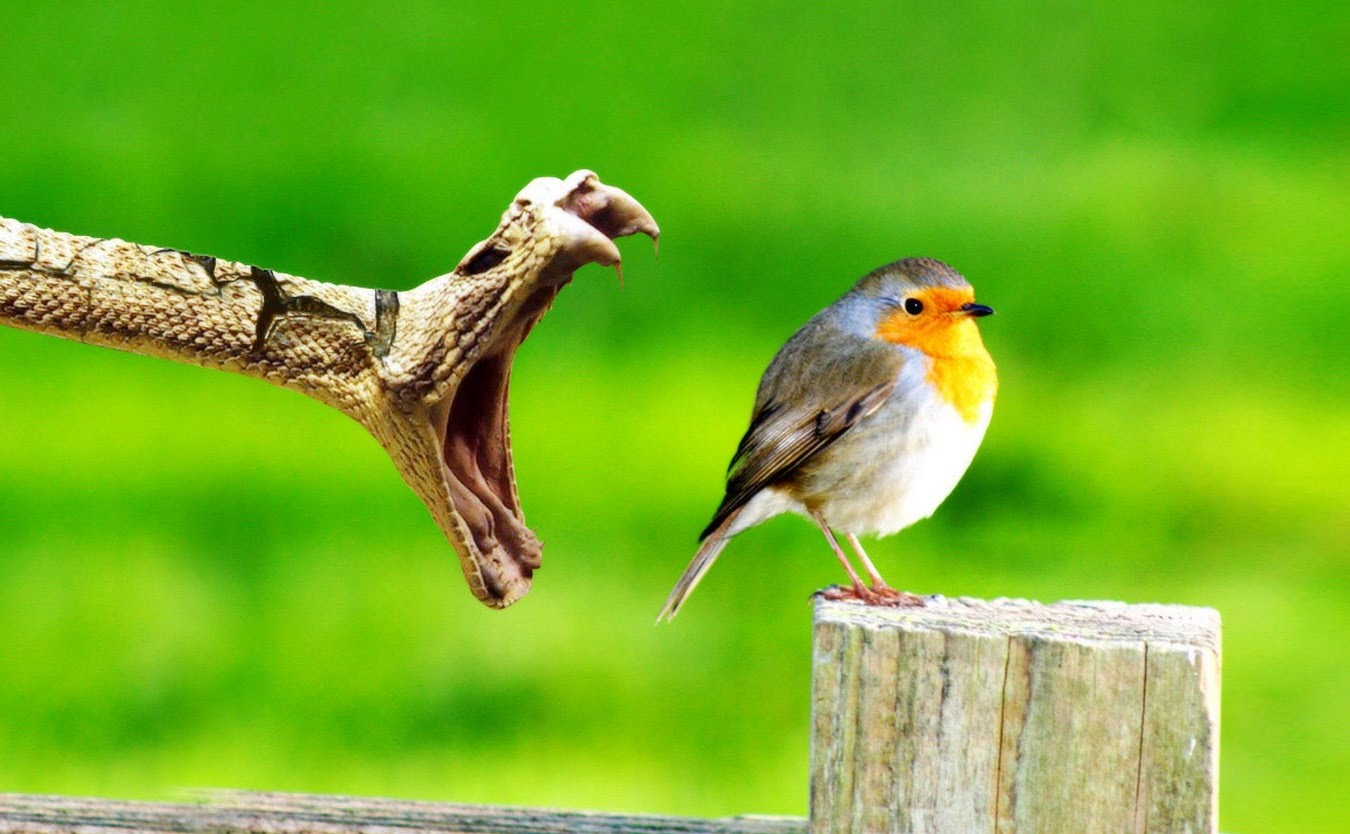
\includegraphics[width=1\textwidth]{Pictures/Example.jpg}	
	\label{forside}
\end{figure}

\vfill
\begin{center}
{ \huge \bfseries {Project titel - edit this in Formalia/FrontPage}}\\[0.2cm]
%{\large \bfseries {}}
\end{center}

% Author and supervisor
\begin{tabularx}{\textwidth}{l X r}
	\hline
	\emph{Authors:} & & \emph{Supervisors:}\\
	Name 1	&	 &	 Supervisor 1 \\
	Name 2     	&	 &	Supervisor 2  \\
	Name 3		\\
	Name 4       \\
	\hline
\end{tabularx}

\vfill

% Bottom of the page
{\large January 2019}

\frontmatter

% \begin{figure}[H]
% 	\centering
% 	\includegraphics[width=0.5\textwidth]{billeder/Matrikelkort.jpg}
% 	\caption{Kort over hvilke matrikler, der henholdsvis er under kommunens og skolens ansvar. Udarbejdet af projektgruppen på baggrund af data fra \citep{Skolematrikel}.}
% 	\label{Matrikelkort}
% \end{figure}
\frontmatter													% Forindhold - nummereres med romertal


\cleardoublepage												% Indsaetter tom side, saa naeste kapitel starter paa hoejre side (hvis noedvendigt)
\pagenumbering{roman}
\setcounter{page}{1}

% \begin{minipage}[t]{0.48\textwidth}
% \vspace*{-25pt}			%\vspace*{-9pt}
% %\includegraphics[height=4cm]{billeder/aau_logo}
% \end{minipage}
% \hfill
% \begin{minipage}[t]{0.48\textwidth}
% {\small 
% \textbf{Tredje Studieår v/ Det Teknisk-}\\
% \textbf{Naturvidenskabelige Fakultet}  \\
% By-, Energi- og Miljøplanlægning\\
% Rendsburggade 6 \\
% 9000 Aalborg \\}
% \end{minipage}

\vspace*{1cm}

\begin{minipage}[t]{0.48\textwidth}
\textbf{Titel:} \\[5pt]\hspace{2ex}
Visualizing and comparing population 
projection rasters

\vspace*{1cm}

\textbf{Projekt:} \\[5pt]\bigskip\hspace{2ex}
Thesis project

\textbf{Project Period:} \\[5pt]\bigskip\hspace{2ex}
February 2020 - June 2020

\textbf{Author:} \\[5pt]\hspace*{2ex}
Andreas Gram Riisgaard 
\\\bigskip\hspace{2ex}


\textbf{Supervisor:} \\[5pt]\hspace*{2ex}
Carsten Kessler \\\bigskip\hspace{2ex}



%\vspace*{1cm}

\textbf{Number of pages:} 71 \\
\textbf{Number of annexes:} 2 \\ 
\textbf{Afsluttet:} 4-6-2020
 
\end{minipage}
\hfill
\begin{minipage}[t]{0.8\textwidth}%483
 \textbf{Abstract:} \\[3pt]
 \fbox{\parbox{8cm}{\bigskip

In this thesis project an interactive tool for visual comparison of raster datasets have been developed using population projections as a case. 

To develop a tool able to enable such comparisons it is important to know how population projections should be visualized and which functionalities are important for the tool. There is a technical challenge in visualizing large raster datasets, while still maintaining a responsive user experience.

The conventions for visualization of population projections was explored through a literature review. A quantitative sequential dataset like a population projection should be colored, so that the areas with least population is colored in a lighter color, than the more densely populated areas. 

The functionalities for the tool was determined by comparing with another interactive map. It was decided to have two maps showing different population projections. The maps can be navigated either by panning and zooming or using a search bar. 

To ensure a responsive user experience the raster was not loaded into the tool in its entirety. Instead it was divided into smaller tiles, which got loaded based on the extent of the map. These tiles were then colored on the client.

The tool was created as an Openlayers map displaying tiles, which was created with a modified version of the python program gdal2tiles.
While the user experience is responsive while using the map the creation of tiles is time consuming. The tool could therefore be improved in the future by using cloud optimized geotiffs instead of tiles.
\bigskip}}
\end{minipage}

\cleardoublepage
\chapter{Preface} 
This is edited in the file Formalia/Preface

\cleardoublepage

%%%% Indholdsfortegnelse (TOC) %%%%

\phantomsection													% Kunstigt afsnit, som hyperlinks kan 'holde fast i'
\pdfbookmark[0]{Indholdsfortegnelse}{indhold}					% Tildeler en klikbar bookmark til den endelige PDF
\tableofcontents*												% Indholdsfortegnelsen (kaldet ToC) 

%\addtocontents{toc}{\protect\newpage}							% Fremtvinger sideskift i ToC hvis noedvendig (der hvor koden placeres)

\mainmatter														% Hovedindhold - nummereres fra side 1

%%%% Rapportindhold %%%% 										% Rapportindholdet boer IKKE indeholde broedtekst - KUN includede filer!

% Opdel evt. i passende afsnit for overblikkets skyld

\chapter{Introduction}

In 2019 the population in the world reached 7.7 billion people, which is an increase of one billion over the past twelve years. According to The United Nations Department of Economic and Social Affairs’ (UN DESA) median scenario the growth is expected to continue reaching 9.7 billon in 2050. \citep{UNDEASHightlights} 

To be able to adapt infrastructures to this population growth it is necessary to predict where these people will settle. While UN DESA provides this information on a national level \citep{NationalPop}, it is more ideal with a more nuanced picture, since most planning are based on local or regional scale spatial projections. \citep{WhyDetailedPop}

Other researchers (SEDAC, CISC) have used simulations to distribute the population within each country as raster layers. However due to the high resolution and/or small scales, visually comparing these raster datasets is a time-consuming task. The purpose of this project is to create a tool allowing fast and easy comparison of such raster datasets, focusing on the use case of population projections.

%Evt noget om at det vil være ekstra interessant at have områderne med stor vækst som case - tilføj her, hvis der skal argumenteres for en case senere

\section{Problem statement}

To explore the possibilities for creating such a comparison tool the following research question have been defined:

\textit{How can population rasters be visualized and compared efficiently and effectively?}

This broad main question will be answered by answering the following three subquestions:

\textbf{Which conventions exist for visualization of population projections?}

\textbf{Which functionalities are relevant for comparing different rasters?}

\textbf{How can a responsive user experience be ensured, when loading and visualizing large raster dataset?}


\section{Limitations}\label{Lim}

Determining relevant functionalities and the responsiveness would ideally have been done with user testing.  However it was determined that both the creation of the tool and a scientific approach to user testing would require too much time.
Therefore the tool creation got prioritised and other evaluation methods were chosen. This is expanded upon in section \ref{Eval}

\section{Target audience}\label{TA}

The target audience for this project is academical researchers. It is meant as a tool for these researcher to be able to quickly compare different population projections. 

This prototype of the tool have only been created for internal and individual use. It will therefore not be created with multiple users in mind and there will be no considerations for security.


The tool is also created with only computers in mind, so it will not be optimized for mobile. 

Alternative target audiences are being discussed in section x.

\section{Report structure}

\fxnote{ADD: quick overview of what the solution is going to be, what is population projections, SSP}

%The report have been divided into three parts. The first part is the literature review, which will address the first two subquestions and also present the two projections visualised in this project. Chapter x explores which conventions there exist for population projections, while the relevant functionalities for raster comparison are detailed in chapter x. Lastly chapter x will give an overview of the population projection SEDAC and CICS, which will be used as case for comparison.
%
%The second part is addressing the last subquestion. First there is a definition of how a "responsive user experience" has been defined. Then different methods of visualising raster datasets are being tested in chapter x. Based on these initial tests a method will chosen, which will be evaluated in the next section.
%
%The last part starts with a discussion in chapter x of the results of the previous part. This is then followed by the last two chapters x and x, which are the conclusion and future work.  

%Part I: Litterature review
%- Conventions, what are relevant functionalities, Explaining the two case projections
%
%Part II: Choice of method
%- Test of different methods 
%
%Part III: Discussion 

The report has been divided into three parts; design, development and evaluation.




In the design part the thought process behind the design of the solution is explained.
It starts with some background information about the case data in chapter x, raster formatting in chapter x and chapter x about how the raster data currently is being compared. 

\begin{figure} [H]
	\centering
	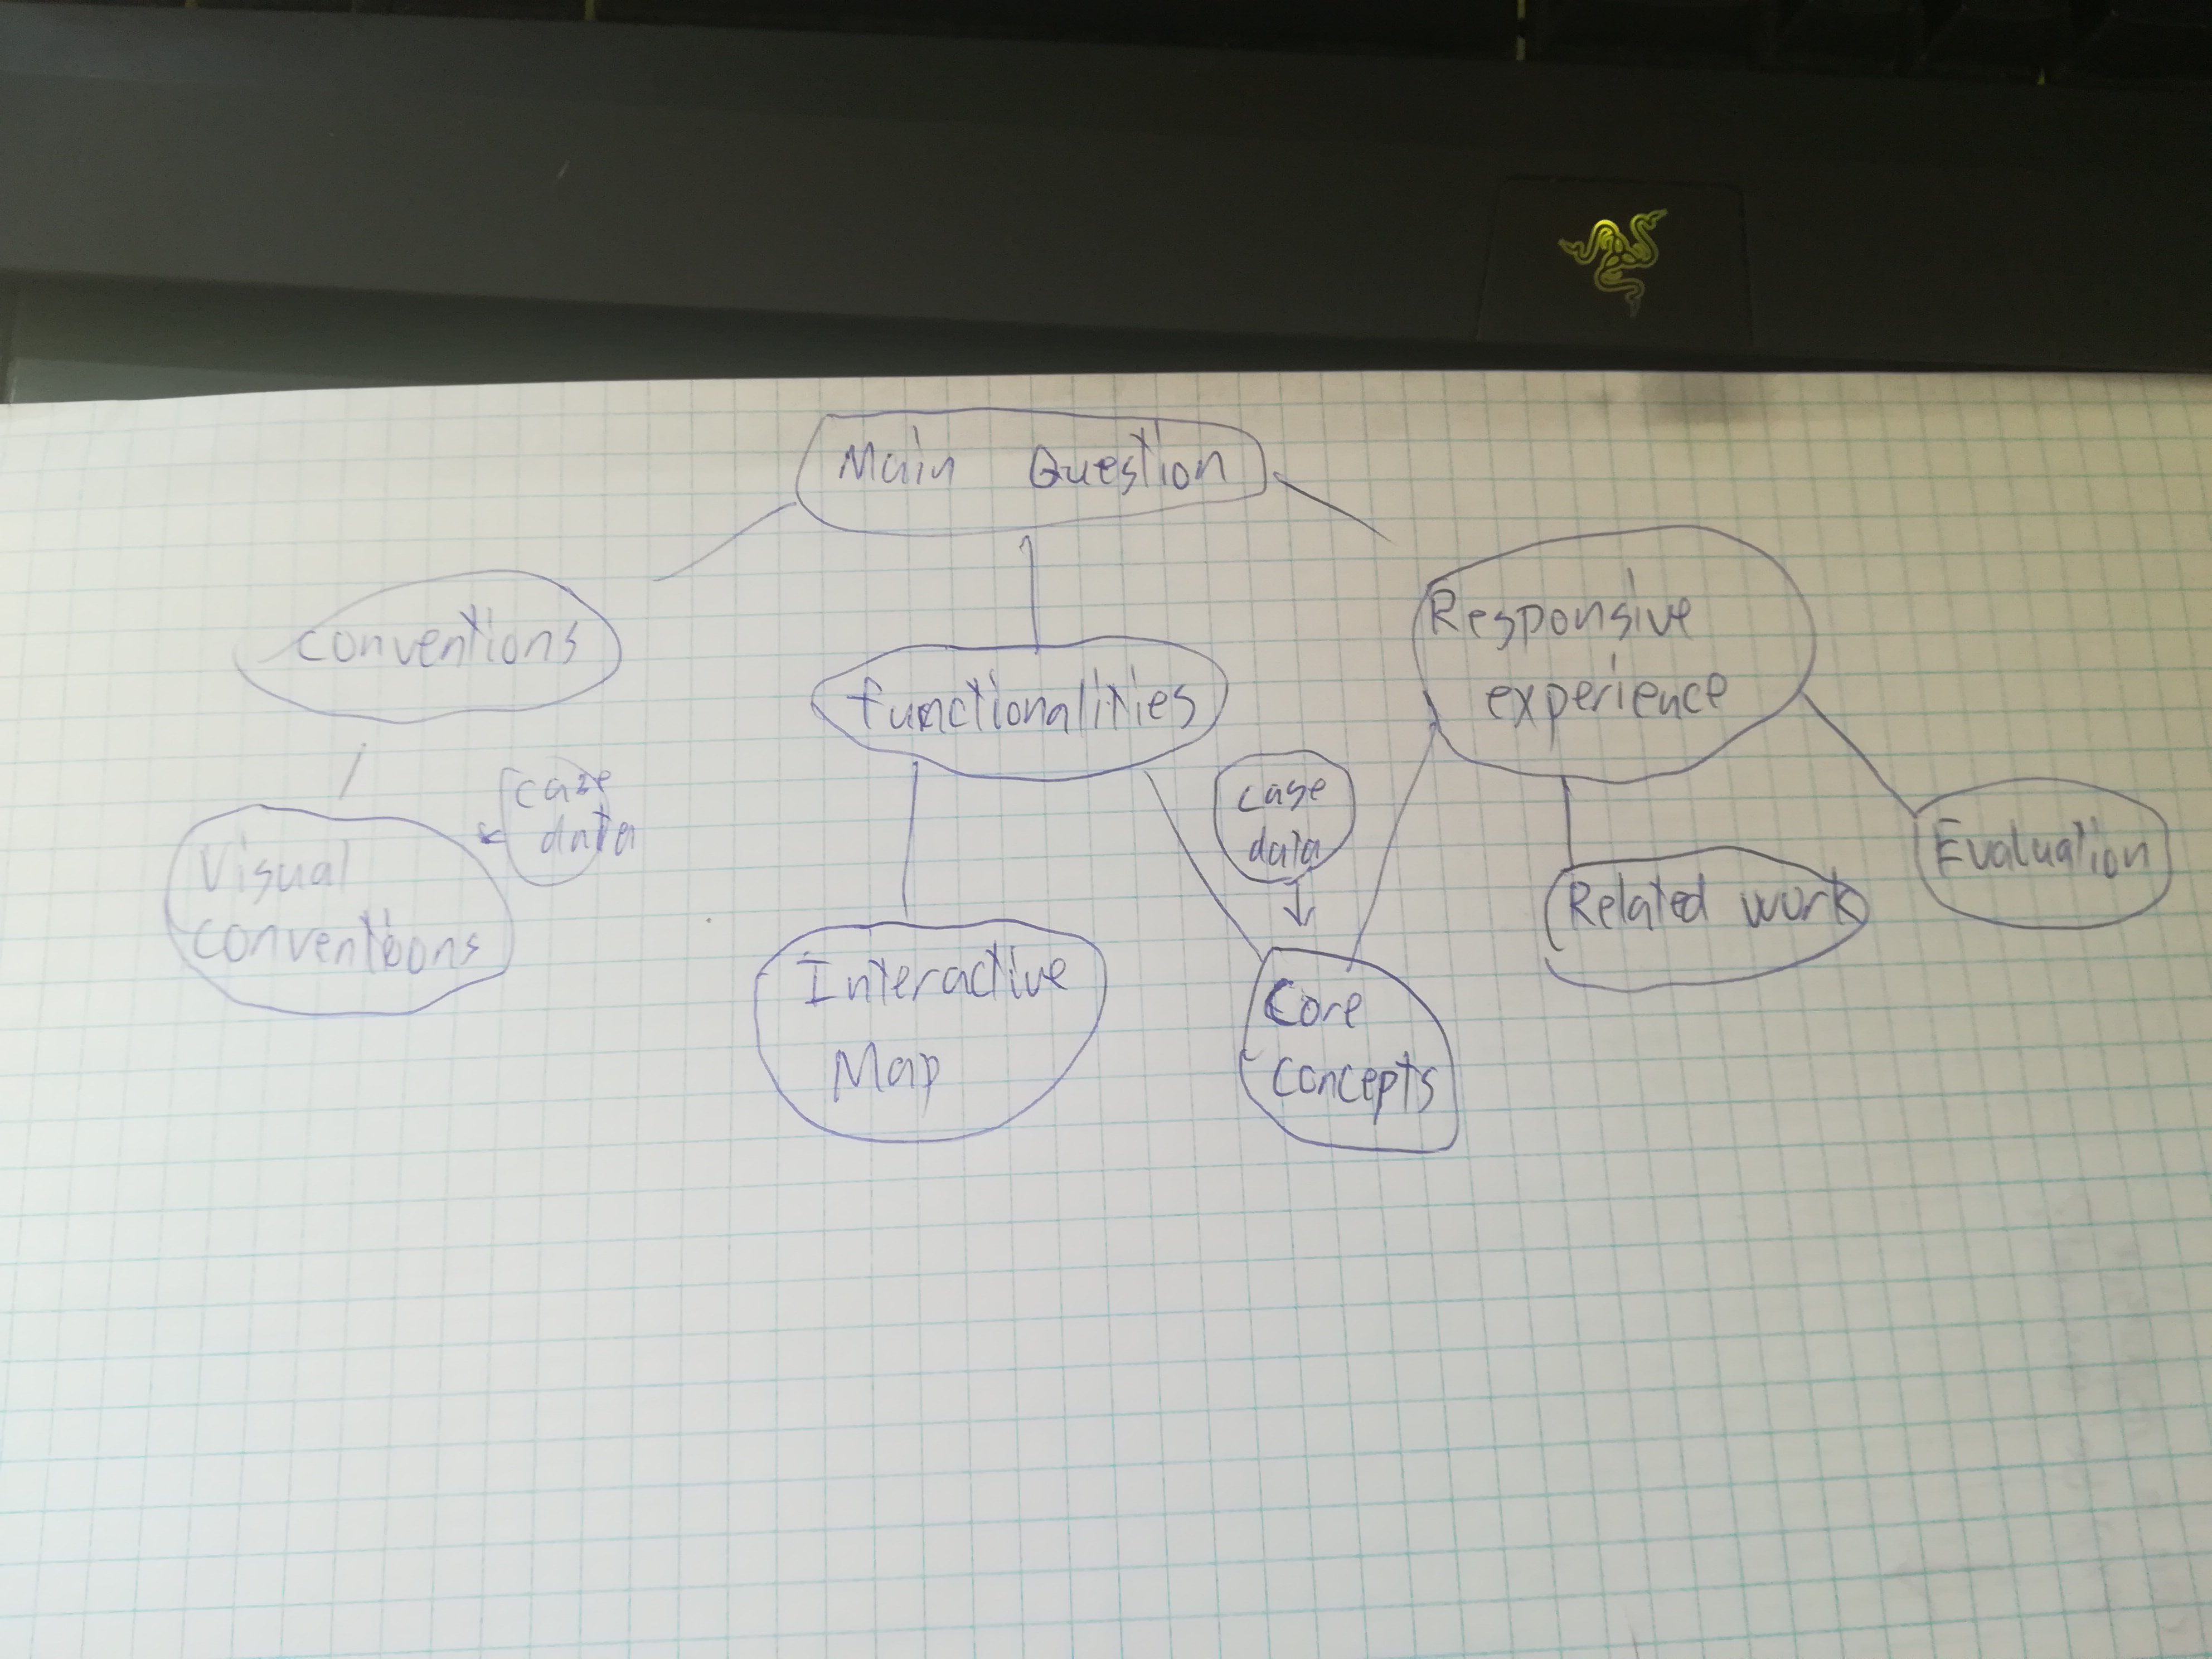
\includegraphics[width=.8\textwidth]{Pictures/Structure}
	\caption{Overview of how the research question gets answered in the first part of the report}
	\label{Structure}
\end{figure}

The rest of the first part is focused on answering the subquestions as illustrated in figure \ref{Structure}. 
The first subquestion is answered through a literature review in chapter x. After the visual conventions have been explained an example of an interactive map gets analysed in chapter x. This is done to understand which functionalities are important for such a map. This is followed by a review of related work in chapter x. Based on the related work and an initial exploration of the data five core concepts for the tool are created. These are described in chapter x. All of the considerations presented in this part then gets collected into the design in chapter x. 

The second part is the development of the tool. In chapter x the building blocks, which the tool is build from, are presented. How these building blocks are put together is then explained in chapter x. Chapter x is an overview of the final product.


The last part starts with an evaluation of the developed tool in chapter x. This is followed by chapter x with a discussion of the tool and how it could be developed further. The last chapter is the conclusion in chapter x 


\fxnote{Add a section, which summerieses the first part}

\part{Design}
\chapter{Case data: Population projection}\label{CCaseData}
The population projection visualized in this project have been created by \citet{Kessler} using a geosimulation, which geographically distribute a predicted population. This geosimulation has been run every tenth year from 2010 to 2100. It has also been run for different scenarios for the future.

\section{The data behind the simulation}\label{TheDataBehind}
This projection is a geographical distribution of the global prospects created by The United Nations Department of Economic and Social Affairs. These prospects estimate the population numbers in each country living in rural and urban areas. The spatial distribution has been based on raster data from the Global Rural Urban Mapping Project (GRUMP). In this dataset the world has been divided into 1x1 km cells, each of which contains the number of estimated people. \citep{Kessler}

The geosimulation has been run with two different definitions for the urban extent. The first one is also created by GRUMP. This urban extent has been estimated based on the light emitted after dark. It is known to overestimates the extent of urban areas. \citep{Kessler}
The second dataset was provided by Global Land Cover Map from the European Space Agency (GlobCover), where areas classified as “artificial surfaces and associated urban areas” in the GlobCover data were treated as urban areas. 

\section{The simulation}
Using this dataset to define the extent of urban and rural areas, the simulation was run as illustrated in figure \ref{CreatingData}.

\begin{figure} [H]
	\centering
	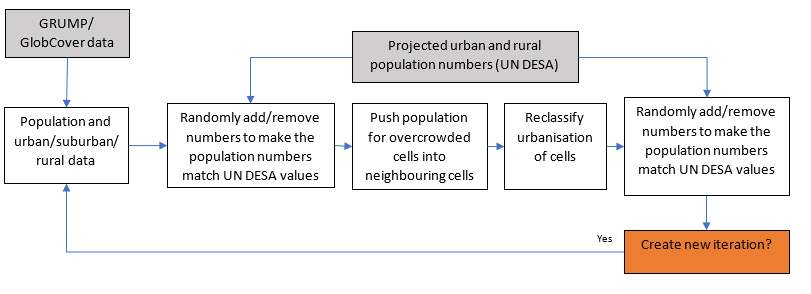
\includegraphics[width=1\textwidth]{Pictures/CreatingData}
	\caption{A flowdiagram of simulation creating the population projections}
	\label{CreatingData}
\end{figure}

The population in rural and urban areas were adjusted to match the projected values from UN DESA. This was done by randomly adding or removing people from the area types. 

The cells would have a country-specific limit on how many people could live in them. Any cells with a population above this limit would push the excess population to neighboring cells. 

After this, the cells would be reclassified as more urbanized if their population had increased above a country-determined threshold. This way a rural cell might become a suburban one or a suburban become urban if its population increased. The data is then adjusted to match projected values again with the same approach as before. This is required because the reclassification would mean that the number for the different urbanization classes would no longer match the numbers from UN DESA.

These steps are then repeated for every iteration. 

\citep{Kessler}
\section{Shared Socioeconomic Pathways} \label{SSPs}

\begin{figure} [H]
	\centering
	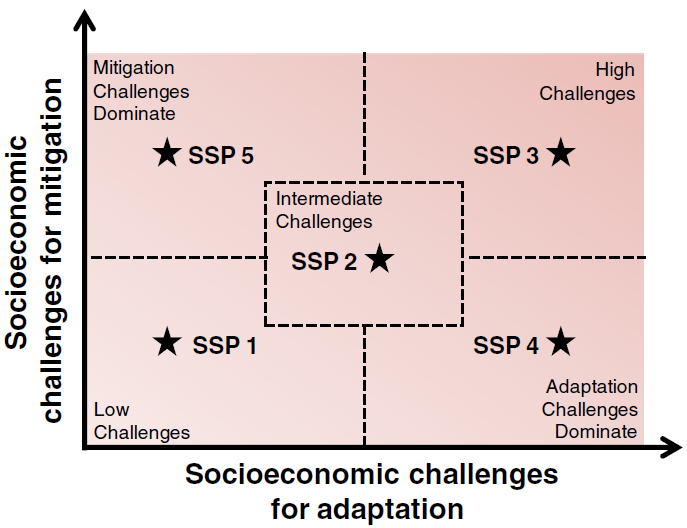
\includegraphics[width=.6\textwidth]{Pictures/SSPAxis}
	\caption{Five different future scenarios based on how clima change could affect society. Source: \citet{ConceptSSP}}
	\label{SSPAxis}
\end{figure}

The geosimulation has been run for five different future scenarios called the Shared Socioeconomic Pathways (SSPs). The different scenarios are based on different ways, climate change could affect society. As illustrated in figure \ref{SSPAxis} the five scenarios are based on two axes: socio-economic challenges for mitigation and for adaptation of climate change impacts. 
“Socio-economic” is referring to a large array of societal and socioecological systems. Covering aspects of a political, social, demographic, cultural, lifestyle, institutional, economic, and technological nature and condition of ecosystems. 
The horizontal axis is environmental or societal conditions, which would make adapting to climate change more difficult. This includes climate hazards (temperature and precipitation changes, sea level rise and extreme weather phenomena) and what and whom these hazards will affect.
\citep{ConceptSSP}
The vertical axis is factors, which in absence of climate policy would increase the amount of emissions of greenhouse gasses and factors reducing the society’s capacity to reduce those emissions. Examples of factors reducing society’s capacity is inadequate technologies and insufficient resources to support mitigation policies. The increase in greenhouse gasses could for example be a result of population and economic growth.
\citep{SSP}

\begin{table}[htbp]
	\centering
	\begin{tabular}{l}
		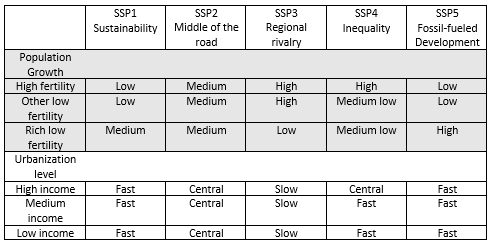
\includegraphics[width=0.8\textwidth]{Pictures/SSPTable}
	\end{tabular}
	\caption{Population growth and urbanization for each of the Shared Socioeconomic Pathways (SSP). Source: \citet{WhyDetailedPop}}
	\label{SSPTable}
\end{table}

How the population growth and the urbanization levels will be in the different scenarios can be seen in table \ref{SSPTable}. The population growth values are based on current income and fertility condition. The urbanization predictions are based on the current income. The Rich low fertility group has been defined as members of the Organisation for Economic Co-operation and Development.


\section{Technical details about the case data}\label{caseDataTech}

Table \ref{tabTech} is highlighting some technical specifications of the dataset, which will be important for the development. The technical details have been acquired using GDAL's raster information program, gdalinfo. GDAL is further described in section \ref{Librarygdal}.

\begin{table}[h]%You have to add this h yourself
	\centering
\begin{tabular}{|c|c|c|}
	\hline 
	\multicolumn{3}{|c|}{Technical information} \\ 
	\hline 
	Attribute & Value & Further explanation \\ 
	\hline 
	NoData value & -2147483648 &  \\ 
	\hline 
	Bit depth & 32 &  Section \ref{BitDepth}\\ 
	\hline 
	Projection & EPSG: 4326 &  Section \ref{ProjectionTheory}\\ 
	\hline 
	Projection unit & Degree &   \\ 
	\hline 
\end{tabular}
\caption{Technical attributes of the case data}
 \label{tabTech}
\end{table}

Some of these concepts will be explained in upcoming sections, but the NoData value will be explained here. A raster file has values for every pixel. If no data is available for a pixel, then the pixel gets assigned the NoData value. \citep{ArcMapOnNoData}

If the value was set to 0 it would be impossible to determine if an area had nobody living in it or if no data was available. That is the reason for the NoData value is set to a negative value, since the population density never can be negative.


\section{Raster formatting conventions}

Aside from the standard connected to the visualization of raster data there are also standard for the formatting of the raster files. Common raster formats include jpeg, png and tiff. One of the key differences between these formats are the bit depth. This value determines how many different colors that can be assigned each pixel in the image. Each bit can only be assigned one of two values, 0 or 1. This number of available colors for a pixel can therefore be calculated as $2^{number of bits}$. As an example, a bit depth of 8 bits would then result in $2^8 = 256$ different potential colors, since is the number of combinations of ones and zeroes, that are possible. For most maps this amount of colors is enough. The human eye can comprehend around 10 million different colors, but often that many colors are not needed. When displaying aerial photographs, the depth of 24 bits is often used, since it can display 16.7 million different colors and therefore can appear in true-colors to humans.
The limitations of the human eye does not mean that having more than 10 million bit combination is pointless. The bit combination can also be used for other thing than colors. It can be used to create transparency values or to store metadata about the image file. For instance, the geotiff format can use the additional bit to store georeferencing information.
These advantages of higher bit count come at a cost of a larger file size. Having a larger color depth will result in a slower loading and larger requirements for storage space.
Dent. 283 
\subsection{Tiled raster}
This section describes standards for dividing large raster files into smaller tiles. 
A way of only visualising the necessary parts of a raster is to divide it into smaller raster tiles and then only load the relevant tiles. When loaded into the map these tiles then gets places next to eachother, so they appear as a single large map image. These tiles can also be created with different resolutions, so that zooming in on the map with return tiles more details.  As illustrated in figure \ref{TilesPerZoomLevel} each of these zoom layers have more tiles.
http://www.liedman.net/tiled-maps/
When zoomed all the way out the entire world is rendered as a single tile. Whenever the zoom level gets increased by one each tile in the previous layer get replaced with four smaller tiles. The number of tiles on a zoom level z can therefore be calculated as $2^2z$

$https://wiki.openstreetmap.org/wiki/Slippy_map_tilenames$


\begin{figure} [H]
	\centering
	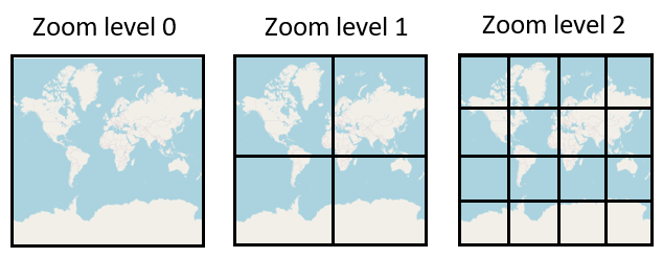
\includegraphics[width=.8\textwidth]{Pictures/TilesPerZoomLevel}
	\caption{Illustration of the increase in tiles for each zoom level}
	\label{TilesPerZoomLevel}
\end{figure}

Openstreetmaps is an example of a service, which use tiled rasters for their map. When this service is used, requests for tiles are send to 
http://tile.openstreetmap.org/zoom/x/y.png
In the request the values zoom, x and y are replaced with the current zoom level, tile column and tile row.
$https://wiki.openstreetmap.org/wiki/Slippy_map_tilenames$

\begin{figure} [H]
	\centering
	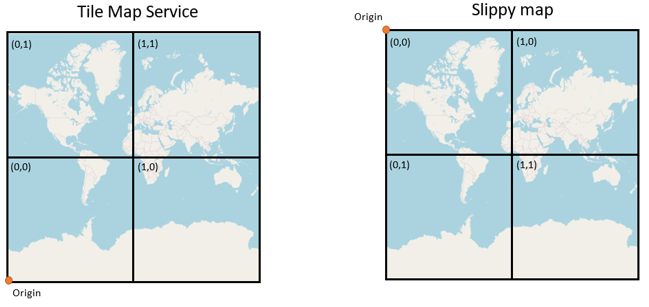
\includegraphics[width=.8\textwidth]{Pictures/TMSXYZ}
	\caption{Illustration of the difference between the TMS and XYZ formats}
	\label{TMSXYZ}
\end{figure}

%https://developers.planet.com/tutorials/slippy-maps-101/ https://wiki.osgeo.org/wiki/Tile_Map_Service_Specification#TileMap_Diagram 

The naming of these tiles are done differently for different standards. In this section only the Tile Map Service (TMS) and Slippy map (XYZ) standard will be addressed. Both of these have the same approach to naming zoom level and columns, but different approach to naming the rows. This difference has been illustrated in figure \ref{TMSXYZ}. The reason for the difference is that TMS tiles number their rows from south northwards, whereas XYZ are numbering rows the reverse way. Due to this difference in numbering rows loading tiles from the wrong standard results in a map as shown in figure \ref{SlippyInTMS}.
https://wiki.openstreetmap.org/wiki/TMS 


\begin{figure} [H]
	\centering
	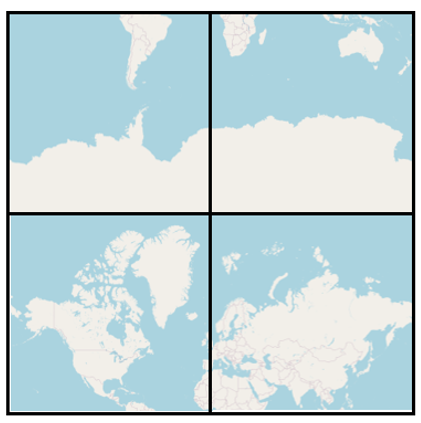
\includegraphics[width=.8\textwidth]{Pictures/SlippyInTMS}
	\caption{How the map looks, when the TSM and XYZ get switched}
	\label{SlippyInTMS}
\end{figure}
\chapter{Current methods of comparing rasters}

When trying to solve an issue it is important to understand what the current methods for achieving the same is. This chapter will present three current methods for comparing rasters

\section{Desktop Gis program}

One way of visualising the population data would be to load the data into a desktop GIS programs like QGIS or ArcGIS. Both of these can visualise TIFF files and it is possible to visually compare different raster layers by changing back and fourth between the different layers. However one would have to manually style the layer to make spatial patterns become visible. Without styling the layer the tiff file will be colorized based on the most and least populated areas in the world. When coloring based on these extremes most of the world will appear in the same color as illustrated in figure \ref{QGIS}. Only the most populated areas in India and china will appear in a different color. This is further expanded upon in section \fxnote{Ref to core concepts}

\fxnote{Remember Carsten mail about locally, on-the-fly and subdomains}
\begin{figure} [H]
	\centering
	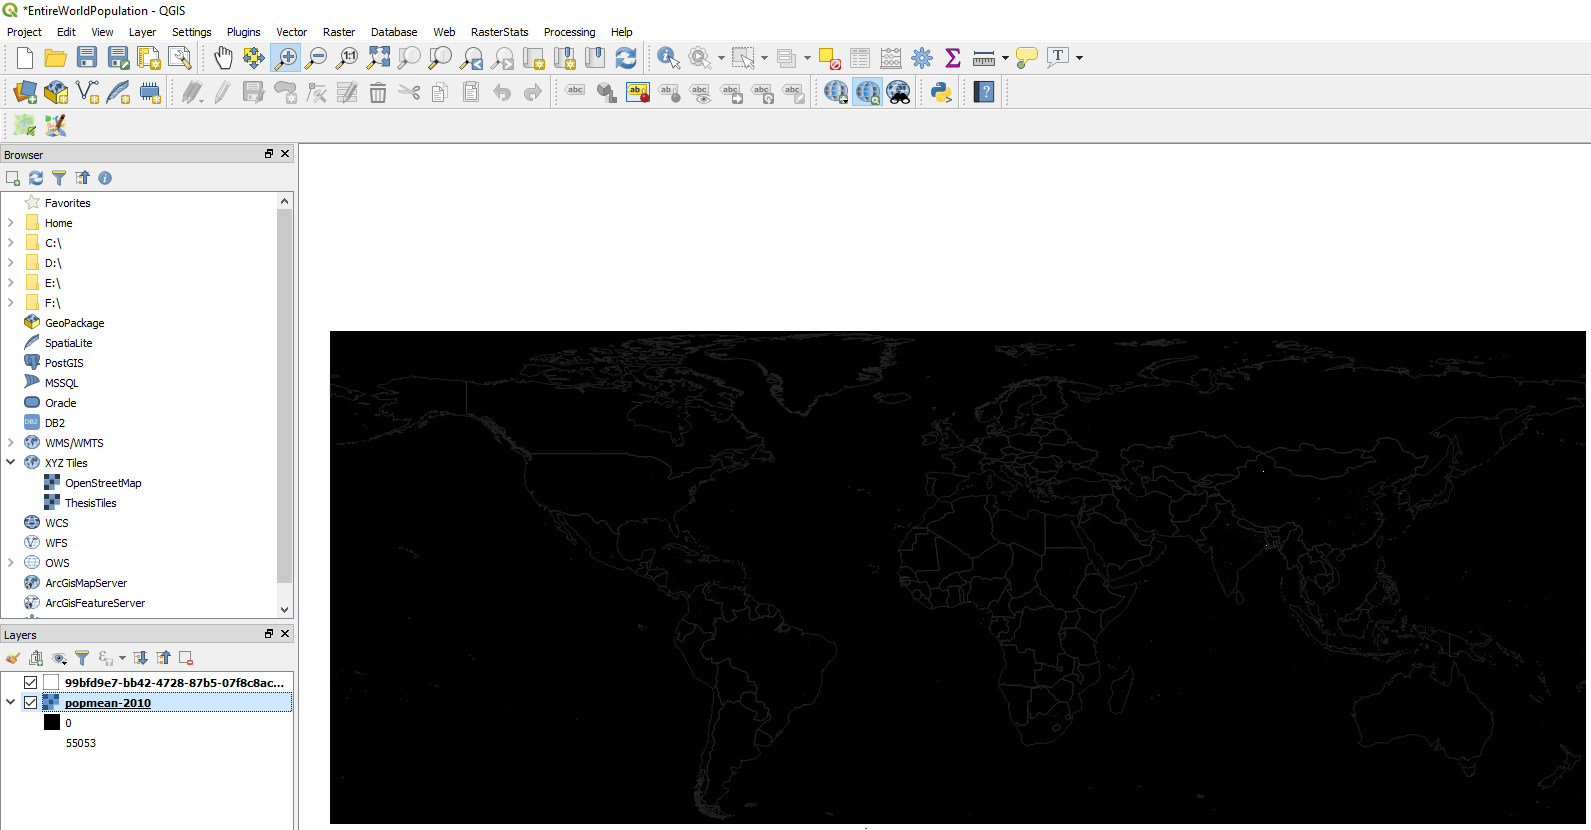
\includegraphics[width=.8\textwidth]{Pictures/QGIS}
	\caption{The population distribution visualised in QGIS and colored based on data from the entire world}
	\label{QGIS}
\end{figure}

\section{Interactive visualization tool for population simulations}

\begin{figure} [H]
	\centering
	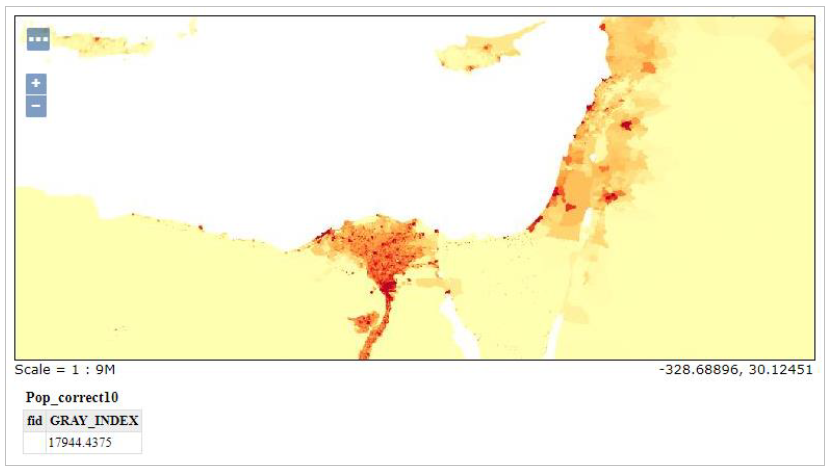
\includegraphics[width=.8\textwidth]{Pictures/Geoserver}
	\caption{An interactive visualization tool made in GeoServer. Source: \citet{Sarah}}
	\label{Geoserver}
\end{figure}

\citet{Sarah} wrote a her master thesis about interactive visualisation of the same population projections, which is the case data for this project. In the thesis she tests different methods for interactive visualisation. The first tests are the python libraries Bokeh and Folium. Both of these are creating interactive webbased maps, but were unable to visualize the population projects due to the file size of the rasters. Therefore other solutions were created using servers for geographic imagery. The servers GeoServer and MapServer were used in the thesis, which both uses Openlayers for their interactive interface. Figure \ref{Geoserver} shows the Geoserver visualisation of the raster data. Figure \ref{Mapserver} shows the Mapserver solution. Both tools required a manual styling.

\begin{figure} [H]
	\centering
	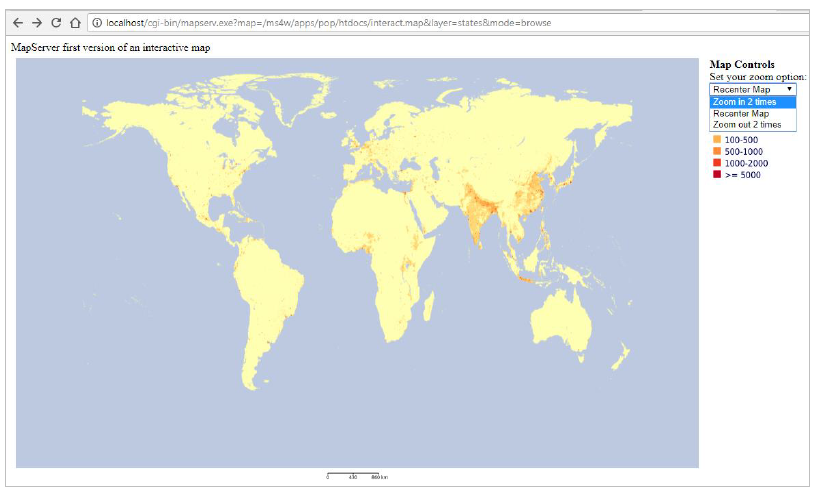
\includegraphics[width=.8\textwidth]{Pictures/Mapserver}
	\caption{An interactive visualization tool made in MapServer. Source: \citet{Sarah}}
	\label{Mapserver}
\end{figure}

The conclusion in the thesis was that MapServer was the faster option, whereas GeoServer had a less steep learning curve. Both servers were slower than viewing in QGIS. Both had limited customizability. As shown in the two figures the tool were only showing a single map and not having and interface for changing the raster layers. The tools were therefore more of an visualization tool, than a comparison tool.


%Sarah 19

\section{MakeCityWebsite}
One of the creators of the case data created a python script, called MakeCityWebsite, for comparing the different population projections for a chosen city.  The final product of the tool can be seen in figure x and x. 

\begin{figure} [H]
	\centering
	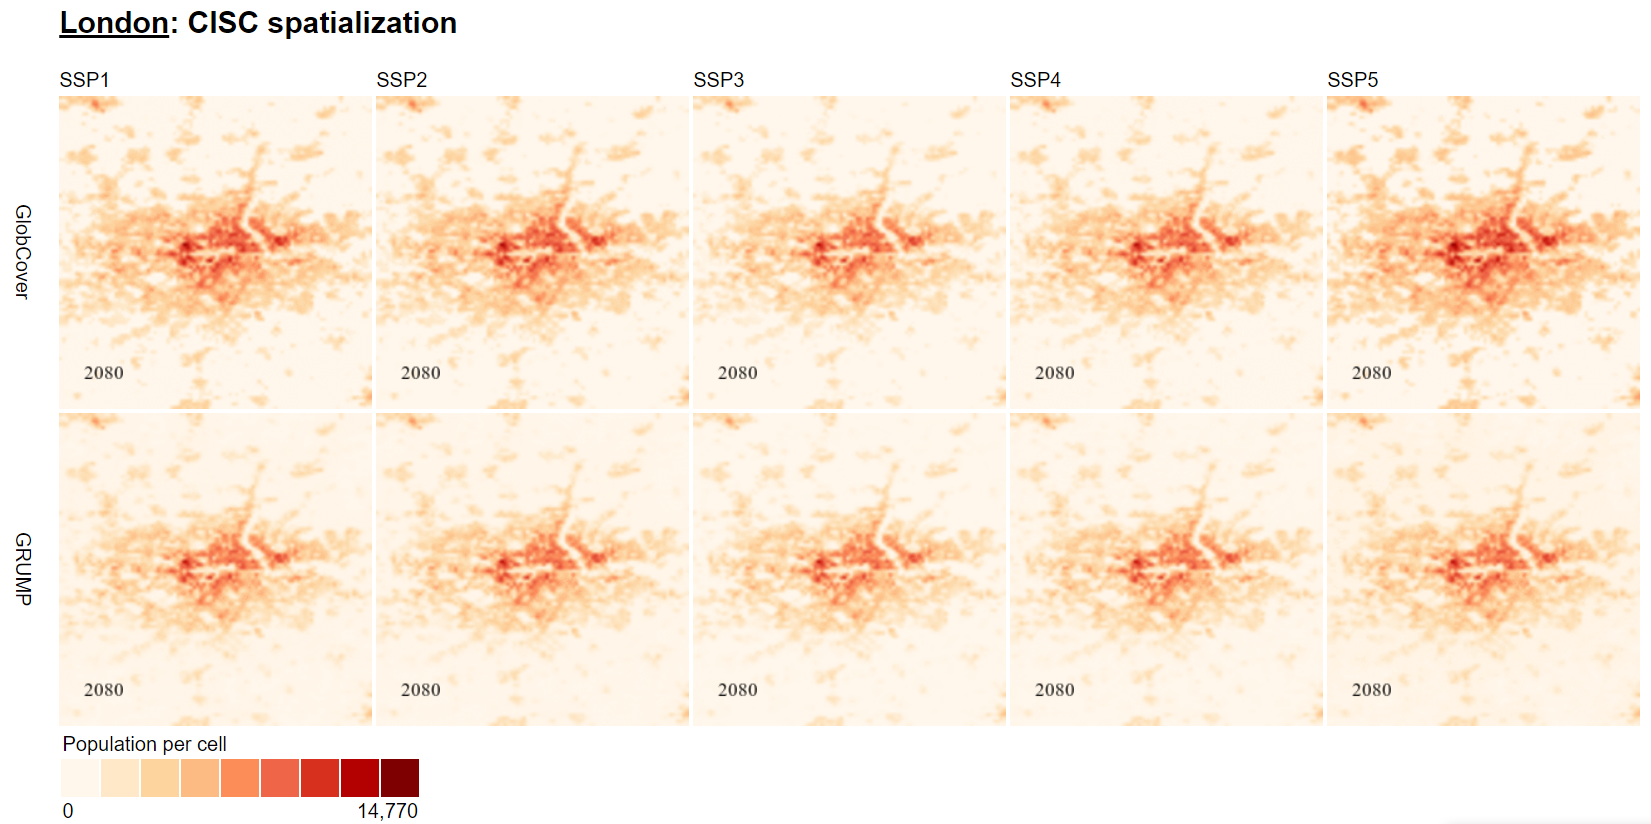
\includegraphics[width=.8\textwidth]{Pictures/MakeCityWebsite1}
	\caption{The top half of a product made by MakeCityWebsite script}
	\label{MakeCityWebsite1}
\end{figure}

The input for the tool is the rasters from each of the two urbanization models, the five SSPs and every tenth year from 2010-2100, so a total of hundred different rasters.
The tool first create new raster files, which have been cut to the extent of the chosen city. Then the minimum and maximum value in those file are calculated. The maximum and minimum values among all the rasters are then used to determine a color scale. This color scale is then used to create a new set of colored rasters.

So at this point the tool have generated one hundred rasters, which all have been colored using the same color scale. For the user to be able to comprehend this amount of data two additional steps are taken. First the individual combinations of urbanization models and SSPs are collected in gifs. These gifs are displayed how the population evolve in their scenario by chronology changing between different years. These different gifs are then placed next to each other in a website as illustrated in figure x. 

\begin{figure} [H]
	\centering
	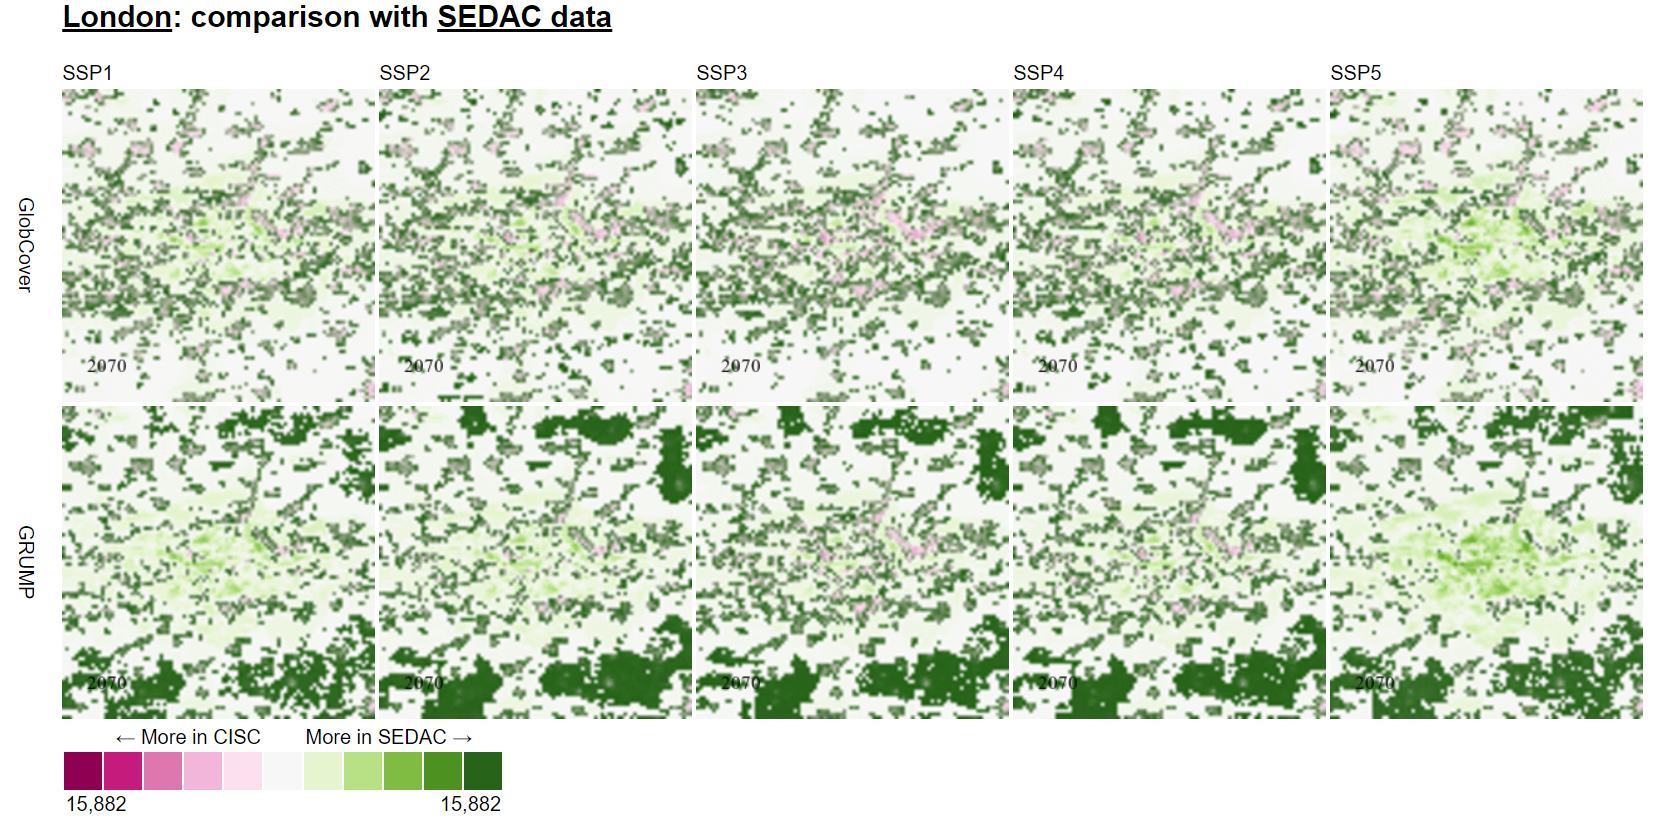
\includegraphics[width=.8\textwidth]{Pictures/MakeCityWebsite2}
	\caption{The bottom half of a product made by MakeCityWebsite script}
	\label{MakeCityWebsite1}
\end{figure}

The tool also creates a comparison with other another population projection called SEDAC. This is done by going though the same steps above, but with a custom raster. This raster visualise the difference between the two projection. This comparison part of the website can be seen in figure z
https://github.com/crstn/CISC/blob/master/MakeCityWebsite.py

The creation of these comparison rasters take 20 minutes for a single SSP
https://github.com/crstn/CISC/blob/master/CompareWithSEDAC.py

\fxnote{How long time does it take to run MakeCityWebsite}




\chapter{Visual conventions}

This chapter will address the visual convention connected to population projection. 
Within the field of spatial convention there are multiple convention, however not all of these are relevant in this particular context. To understand which conventions are relevant for visualizing data one must understand the properties of the data to be visualized. Spatial data can be presented as either discrete-objects or continuous-fields also known as vector and raster data. \citep{objectsNFields} These two types of data have different ways of being visualised. 
As mentioned in chapter \ref{Add chapter} the data is in the raster format and is sequential. Visual conventions connected to discrete-objects will therefore not be covered.

Visual conventions connected to raster maps are largely covered by convention connected to color. 
\subsection{Color}
A color can be defined by three parameters: hue, saturation and lightness. These different concept have all been illustrated in figure \ref{MunsellColorSystem}.

\begin{figure} [H]
	\centering
	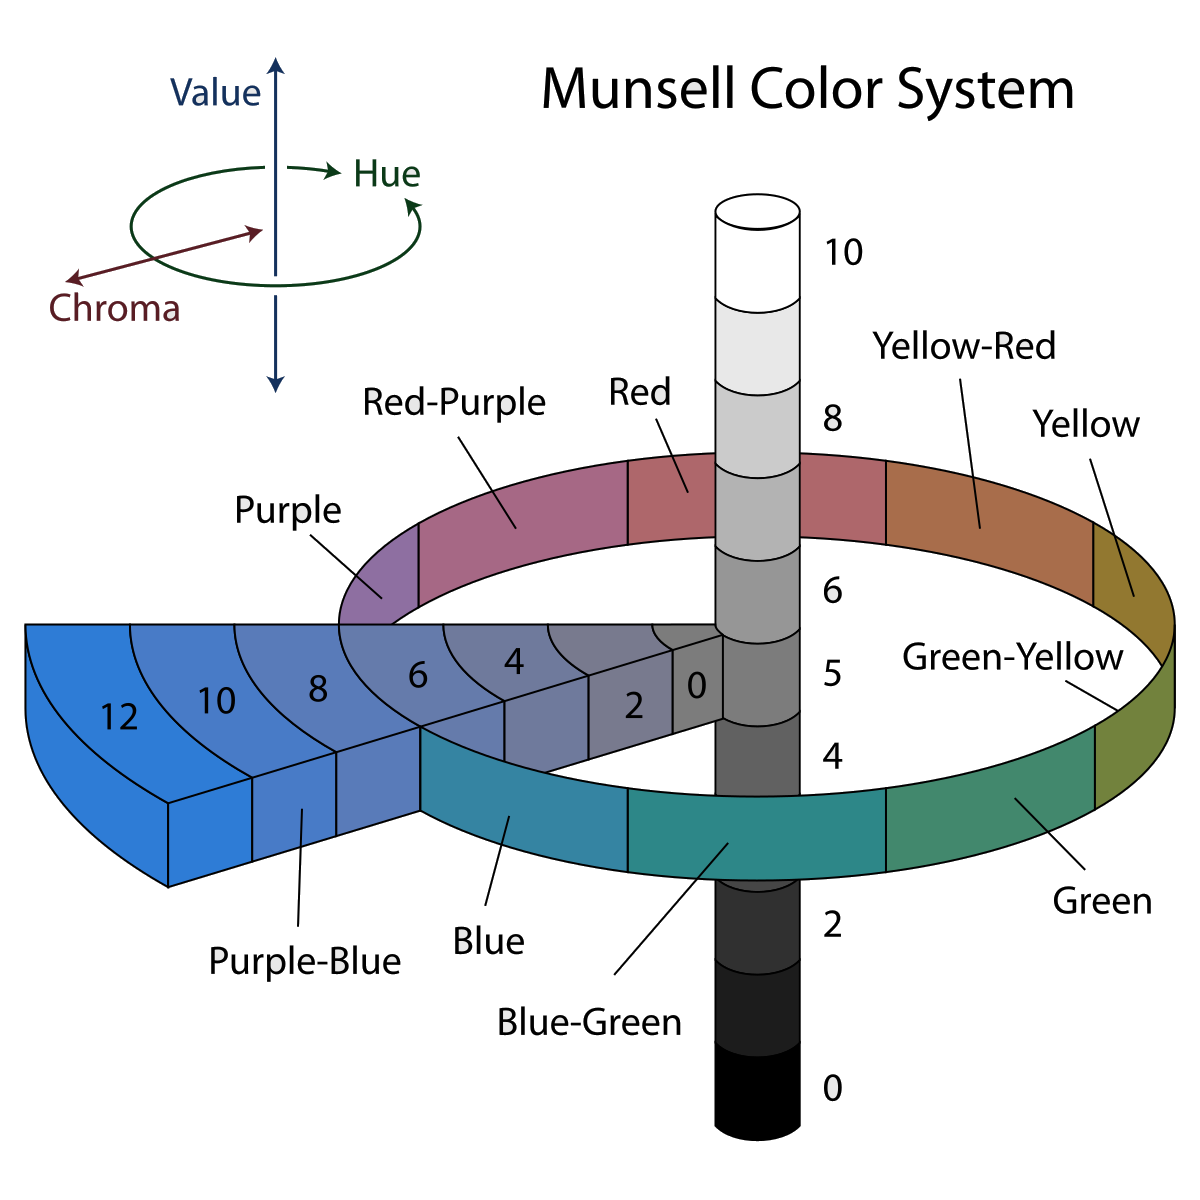
\includegraphics[width=.8\textwidth]{Pictures/MunsellColorSystem}
	\caption{Illustration of the concepts: hue, saturation and lightness}
	\label{MunsellColorSystem}
\end{figure}

\textbf{Hue}

The hue is what would traditionally be referred to as colors (red, green, yellow). In the figure the hue is illustrated as the circle around the column.

\textbf{Saturation}

The saturation is also referred to by some authors as chroma, intensity or purity. It is a measurement for how vivid the color is. A color with a low saturation would be close to the color grey. If the saturation increases more of the color pigment is added to the color, until there is no trace of grey left. The saturation has a value from 100\% (fully colored) to 0\% (grey). It is illustrated in the figure as the distance from the center.

\textbf{Lightness}

A measurement of the color’s lightness or darkness. In the literature this is often referred to as the colors value, but Brewer remarks that this use of terminology is not ideal in data science since "value" also could refer to the data values. It is illustrated as the vertical axis in the figure.  \citep{Dent}

 
\subsubsection{Selecting a color scheme}
There are multiple elements, that should be considered, when choosing a color scheme.
Naturally the different colors should be easily distinguishable, but one should also consider the user of the map and the medium used for presenting the map. The right choice of color pattern allows the user to see patterns in complex data, which otherwise would be obscured. 


Cindy Brewer divides color schemes into the four categories; binary, qualitative, diverging and sequential. These categories and combinations between them have been visualized in figure \ref{BrewerDataTypes}. \citep{Brewer94}

\begin{figure} [H]
	\centering
	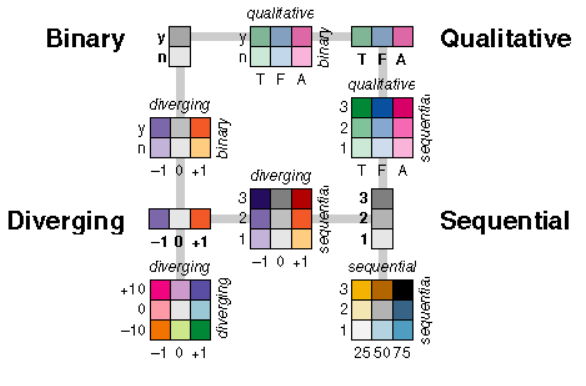
\includegraphics[width=.8\textwidth]{Pictures/BrewerDataTypes}
	\caption{Illustration of the different categories of color schemes. Source: ColorGuidelines}
	\label{BrewerDataTypes}
\end{figure}
 

Each of these categories are good for visualizing different kinds of data. The qualitative is well suited for illustrating nominal data. This color scheme is for instance commonly used for land use maps. The binary scheme is a qualitative scheme, but with only two categories. A example of a use case for this scheme could be visualizing whether countries are members of the European Union or not. 
The sequential scheme is useful for illustrating the ordered data going from low values to higher ones. An example of this could be height of vegetation. The differentiation between the values are illustrated with differences in lightness.
The diverging scheme is similar to having two sequential color schemes. This enables highlighting a critical value in the middle of the data. It is for example being used to illustrate temperatures, where the neutral middle value would be 0$^o$C. \citep{Brewer94}


Based on these categories of color schemes Brewer have developed an online tool, colorbrewer2.org, which can aid mapmakers in picking a color scheme. This tool also takes into colorblindness into consideration and inform the user if a colorscheme is suitable for printing or viewing on small screens. 


%https://colorbrewer2.org/


\subsubsection{Visual conventions for colors}
The conventions can be divided based on whether the visualized data is qualitative or quantitative. The qualitative datasets have many historical convention – like using green colors for vegetation or using blue for water. 
It is not the same case for quantitative data, where “No conventions exist for color choice on quantitative maps. (for example, population density maps are always blue, income maps are always green, and so on)” \citep{Dent}. There are however convention for the choice of lightness, where "light is less - dark is more"
% http://www.geo.uzh.ch/~sara/pubs/garlandini_fabs09.pdf








%
%
%
%\chapter{Initial research and related work}
%
%Prior to developing the tool some initial experimentation with the case dataset was conducted. This lead to some core concepts which should apply to the developed tool. After this existing tool is described, which follows many of these core concepts.

















\chapter{Components of an interactive map}\label{CInteractiveMap}
When creating an interactive map one must consider which features to add to enhance the user experience. To give an overview of some of the basic features used for navigating and get information from a interactive map www.openstreetmap.org has been used as an example. \citep{OpenStreetMap} A picture of this map can be seen in figure \ref{InteractiveMap}. Its User Interfaces (UI) have been numbered with boxes. These boxes have been colored based on how useful the function would be for exploring and comparing large population dataset. The green are essential, the yellow are useful and the red are not relevant. The reasoning behind the coloring is explained in section \ref{SortingFunctions}.


\begin{figure} [H]
	\centering
	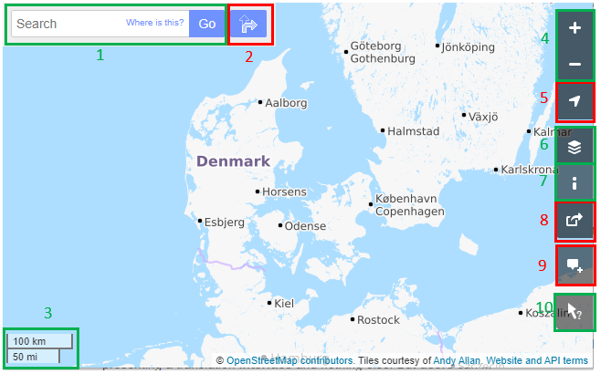
\includegraphics[width=.8\textwidth]{Pictures/InteractiveMap}
	\caption{An example of an interactive map, Openstreetmap. The user interface components have been colored green if it is deemed useful for the developed tool or otherwise red. Source: \citep{OpenStreetMap}}
	\label{InteractiveMap}
\end{figure}



What the different parts of the UI do can be seen in table \ref{tabOSMFunctions}. The functions of the UI can be classified in five different categories. Using the map navigation UI the user can control which part of the map is being displayed.
The real-life navigation tool is used for navigating in the real world. 
The map explanation category gives the user information about the map. This can be general information about the scale or symbols on the map or specific information about a clicked point. 
The tool for controlling the displayed data is used for controlling what is being visualized on the map. The last category, communication with others, is for sharing information with other users of the map. 

\begin{table}[h]
	\centering
	\begin{tabular}{l}
		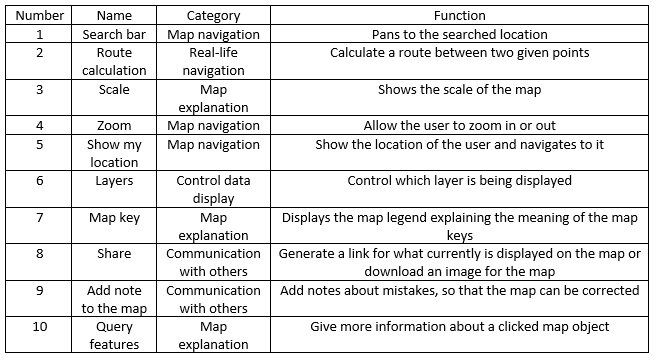
\includegraphics[width=0.8\textwidth]{Pictures/tabOSMFunctions}
	\end{tabular}
	\caption{Overview of the UI elements highlighted in figure \ref{InteractiveMap}}
	\label{tabOSMFunctions}
\end{table}

\section{Relevant functionalities}\label{SortingFunctions}

The essential functionalities are the searchbar, zooming and Map key. 
Having a search bar allows the user to quickly pan to an area of interest and the zoom function allows the user to control the extent. Having a legend is also central to explain to the user which values the colors of the raster would correspond to. 


The useful functions are the scale, the layer control, parts of the share function and the Query features. A scale can help the user get a sense of scale. However, this is only useful if the scale is presented with a unit, which the user easily can comprehend. As mentioned in section \ref{caseDataTech} the unit of the projection is in degrees, which would result in the scale also being in degrees. The layer control is important, since this would allow the map to be able to display multiple different population projections. The tool have been developed for single individuals, so the communicating with other is outside of the scope of this project. However it could still be relevant for a single user to be able to save an extent or export an image of the map. Getting more information about a clicked point could also be a beneficial feature. This information could for instance be the exact value in the clicked point. 

The functions which are irrelevant are the route calculation, "Show my location" and "Add note to the map". The first is only useful for route planning, which is not the purpose of this map. The "Show my location" function is not relevant for this target audience. It would be relevant if the target audience was citizens, who just wanted to explore a population projection out of curiosity. These would potentially be interested in knowing what the expected population would be in their neighbourhood. The last function rely on multiple users, which is outside the scope of this project.

\section{Comparing layers}

The functions presented so far does not enable an easy visual comparison of raster data. It is possible currently by changing back and forth between different layers with different population projections. This however is a bit inconvenient. 
An alternative way would be to use comparison layers in a similar fashion to how it currently is being done with the makeCityWebsite tool mentioned in section \ref{MakeCitySection}. This would require the creation of comparison layers for each combination of SSPs and years, which should be compared.   
A third option would be to display multiple maps at the same time as illustrated in figure \ref{DualMapExample}. These two maps are linked together by a shared view. The means the panning or zooming in one map would do the same operation on the other map.

\begin{figure} [H]
	\centering
	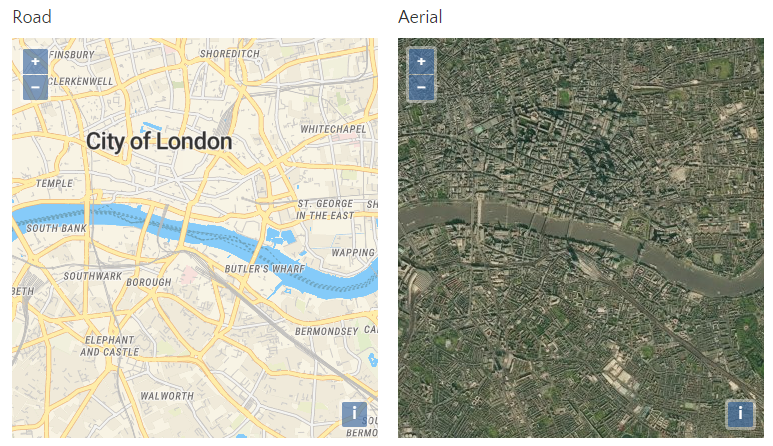
\includegraphics[width=.8\textwidth]{Pictures/DualMapExample}
	\caption{An example of two maps sharing the same view. Source: \citet{DualmapExample}}
	\label{DualMapExample}
\end{figure}


This third option was chosen.
\chapter{Related work}
\fxnote{Write about Cloud optimized Geotiff somewhere}
\fxnote{Write about gdal2tiles parallelly}

This is not the first project attempting to visualising large raster datasets in an interactive way. It is also not the first attempt at visualizing this particular dataset. 

\fxnote{Write about Sarahs stuff here}

\section{Tilebased raster visualisation}

This is not the first project to follow many of these core concepts. In Bernhard Baumrocks master thesis, he created a webmap, where raster tiles were being colored locally. \citep{Baumrocks}

\fxnote{Rewrite into after sarah}
\begin{figure} [H]
	\centering
	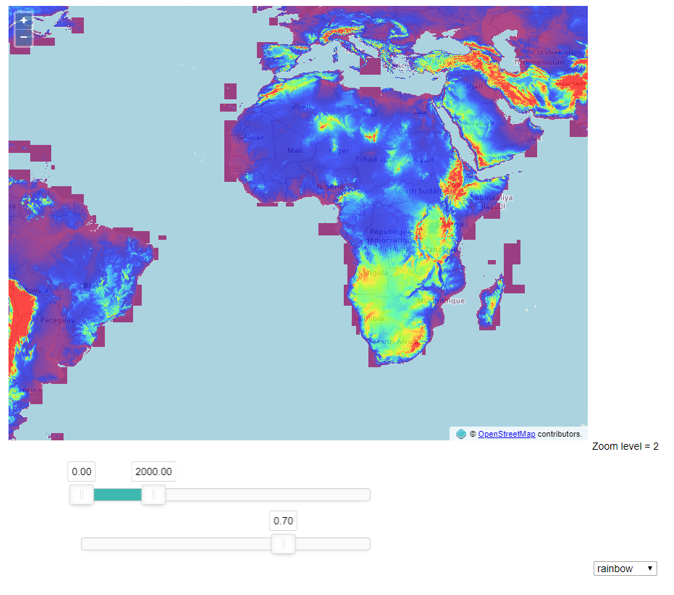
\includegraphics[width=.8\textwidth]{Pictures/BaumrockMap1}
	\caption{The map created by \citep{EOX}}
	\label{BaumrockMap1}
\end{figure}

A picture of one of his maps can be seen in figure \ref{BaumrockMap1}. This particular map is not included in his thesis, but it is the most similar to this project. The map shows an elevation data . Below the map are two sliders and a dropdown list with the label “viridis”. Changing the value in this dropdown list allows the user to switch to another color scheme. The bottom slider is controlling the opacity for the raster layer. The upper slider controls which maximum and minimum values the coloring should be based on. How the map change, when changing the values in the upper slider can be seen in figure \ref{BaumrockMap2}. When zooming in another more detailed layer gets loaded and rendered.
\begin{figure} [H]
	\centering
	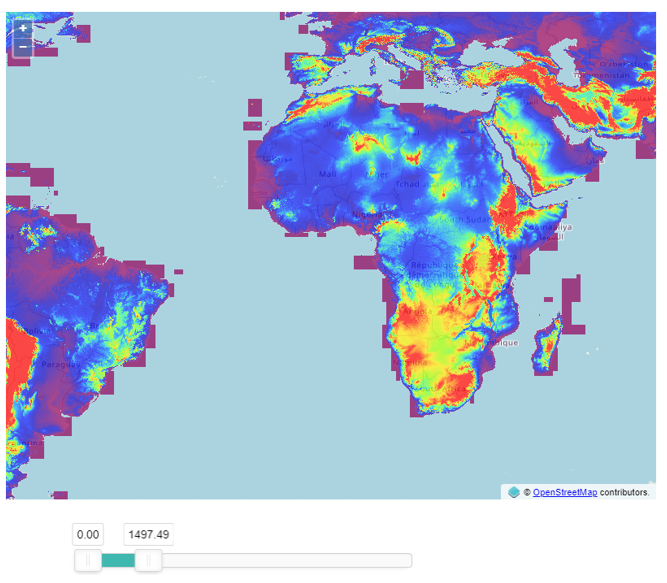
\includegraphics[width=.8\textwidth]{Pictures/BaumrockMap2}
	\caption{How the map change, when using the slider}
	\label{BaumrockMap2}
\end{figure}

%http://webportals.ipsl.jussieu.fr/ScientificApps/dev/forge_patrick/eox/map_01.html

When taking a closer look at the source code it can be seen that the raster is being loaded as tiff tiles with a bit depth of 16 bit. \citep{EOX} Only tiles the currently are visible are being requested unless the tile already have been requested. \citep{Buamrocks}

%When comparing with the core concepts for this project, Baumrocks map fulfil most of the criteria. It is locally visualizing only the necessary data. The core concept related to bit depth is relevant in the creation of the tiles, so it does not really apply to this. 
%It is also to some extent allowing the user to color the layer based on the current extent. The user can adjust the maximum and minimum values but does not know what the maximum values are in the current extent. 
How the tool functions from a technical perspective is further detailed in section x.


\chapter{Technical concepts}
Five technical concepts have been developed based on the current solutions, related work and initial tests with the case data:
\begin{itemize}
	\item Load only the needed data
	\item Coloring should be based on the current extent
	\item Tiles should not be precolored
	\item Coloring should be done locally
	\item File format should have same bit depth as input format
\end{itemize}

The purpose of these concepts is to ensure that a large dataset can be loaded and visualized correctly. 

\section{Load only the needed data}
The case data presented in chapter x holds information for the entire world. However, loading data for the entire world would be unnecessarily time consuming. Initial experiments of rendering this quantity of data also revealed that the browser did not have enough memory to load that amount of data. Instead only the relevant data should be downloaded. The relevant data in this case would refer to the data, which the user is able to see. Getting a subset of a raster dataset can be accomplished by dividing it into smaller tiles. Section x will present two different ways this can be achieved.

\section{Coloring should be based on the current extent}\label{ColorFromCurrentExtent}
The initial exploration of the data showed that the coloring of the tiles should be based of the current extent. This is due to how much the values are varying across the world. Figure \ref{WhyLimitToExtent} shows an example of the difference between a map where the coloring is based on all values or if it is limited to the current extent. Both maps illustrate the population in Denmark. The left map has its coloring based on values from the entire world, while the right has its colors based on the current extent. The left map appears to have no population since the population density in Denmark is negligible compared with the most densely populated areas in the world. In the right map it is possible to see the location of the most populated cities. Since the left map provide the user with no relevant information and the right one does, the coloring should be based on the current extent.


\begin{figure} [H]
	\centering
	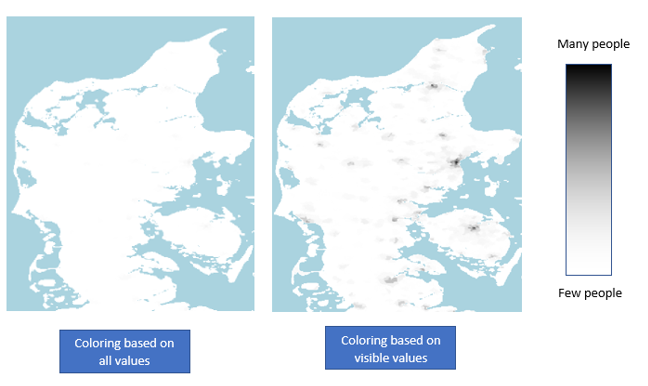
\includegraphics[width=.8\textwidth]{Pictures/WhyLimitToExtent}
	\caption{Population density in Jutland}
	\label{WhyLimitToExtent}
\end{figure}


\section{Tiles should not be precolored}
If the coloring should be based on the current extent and the map is interactive the coloring of the tiles should be done on the fly instead of once and for all. The reason for this is best explained with the example in figure \ref{WhyNotPrecolor}. This figure is illustrating the population in a small subset of India.  The three boxes are illustrating examples of possible map extents, which the user could get by zooming in on different parts of the map. Each of these three have a different max value in their cell with the highest population. The blue square is covering the city center of Indore therefore has a high value than the green, which is covering the outskirts of the city. The last square does not include any part of a bigger city and therefore have a lower value. 
Since their max values are different, they would each need their own coloring. If the tiles were to be precolored it would be necessary to create three coloring of the tiles – one for each the extents. However, since the map is interactive, the extent is not limited to those three. If the user instead were to zoom in on an area between the red and blue square a new max value would maybe be found. When scaling this example up to the entire world and to multiple zoom extents there would be thousands of combinations. If all of these needed to be prerender it would both require lots of initial processing time and storage space for an immense amount of data. 


\begin{figure} [H]
	\centering
	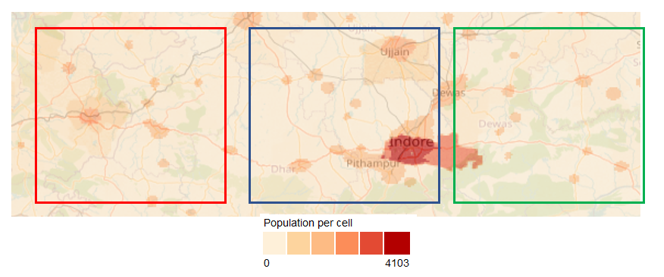
\includegraphics[width=.8\textwidth]{Pictures/WhyNotPrecolor}
	\caption{Population density. The three boxes are examples of possible extents an interacting user could get by zooming.}
	\label{WhyNotPrecolor}
\end{figure}

The alternative is to color the tiles on the fly. When the user would zoom to a new area the map, a script could register the highest currently visible value. This information could then be sent to recoloring script, which would color the tiles based on this. This way only tiles with the needed colors would be rendered. 


\section{Coloring should be done on the client}
The coloring can be done in two ways as illustrated in figure \ref{WhyColorLocally}. It can be done by sending the information to a tileserver, which then would color the tiles and send them to the client. Alternatively, the coloring could be done on the client. 

\begin{figure} [H]
	\centering
	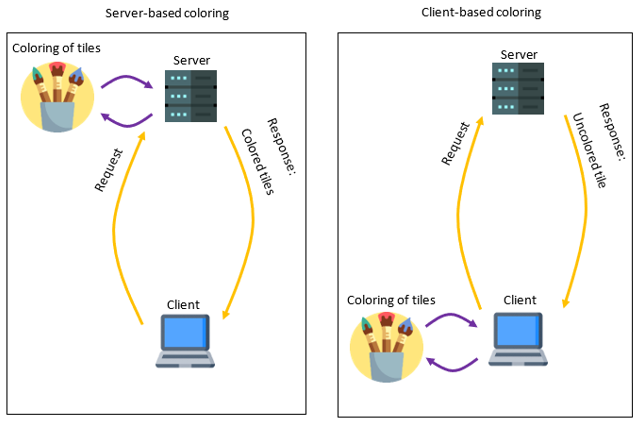
\includegraphics[width=.8\textwidth]{Pictures/WhyColorLocally}
	\caption{Difference between coloring the tile on the server and client. Inspired by a similar looking from \citet{Baumrocks}}
	\label{WhyColorLocally}
\end{figure}
\fxnote{Iconography source}
Comparing the two options is best done with an example, which has been illustrated in figure \ref{WhyColorLocallyMap}. Here the blue and green box are two different possible views both containing 16 raster tiles. The two boxes have different max values, since blue one contains the city center. In the example a user will pan from the blue view to the green one. If the coloring is done on the server side the initial 16 tiles in the blue box will be requested on load.Then when the user pan to the green view the 16 tiles in that box will be requested and colored. The four tiles that are shared between the blue and the green boxes must be requested again, since they need a new color due to the change in max value. This is not the case if the coloring is done locally. In this case only 12 tiles would have to be requested, when changing from the blue to the green view. Since the coloring is happening locally the coloring script can recolor the four tiles it already has downloaded from the initial load.  In the right part of figure \ref{WhyColorLocally} the yellow loop would be run 12 times, whereas the purple one would be run 16 times. This should result in a faster experience for the user.

\begin{figure} [H]
	\centering
	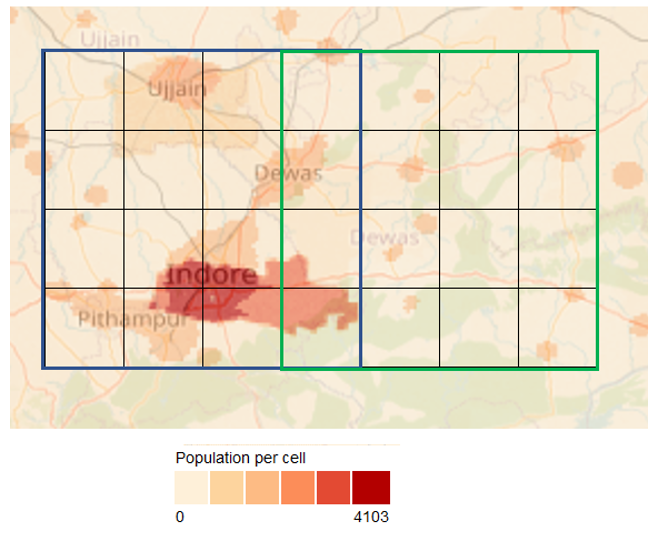
\includegraphics[width=.6\textwidth]{Pictures/WhyColorLocallyMap}
	\caption{Example of why local coloring is needed. The squares are different extents used for the example}
	\label{WhyColorLocallyMap}
\end{figure}

\section{File format should have same bit depth as input format}
As mention in section x the data from the case has a bit depth of 32 bit. To visualize the data the file format must not be changed to a format with less than 32 bits. Figure \ref{WhyNot8Bit} is an example of how a subset of the case data look originally and when converted to an 8-bit format. As mentioned in section x the pixels in an 8-bit raster can have values between 0-255. This means that this format is unable to correctly display the original data range, where the data range is covering thousands of values. The original data get clamped into the 8-bit format producing wrong result
https://gdal.org/programs/gdal2tiles.html .

\begin{figure} [H]
	\centering
	\includegraphics[width=.6\textwidth]{Pictures/WhyNot8Bit}
	\caption{32 bits cramped into 8 bits}
	\label{WhyNot8Bit}
\end{figure}

Normally this issue could be worked around by rescaling the input data to the new format \citep{gdal2tilesDoc} . This rescaling would be a lossy compression resulting in loss of information since the original data cannot be expressed with values between 0-255. \citep{Dent}
For the normal use of tiles this would not be a problem since tiles would only be used for visualization. 
If the tiles are being recolored locally the tiles are being used for more than just visualization. It is necessary to access the data within the tile. This means that solutions resulting in a lossy compression are not an option. To ensure that the correct data reach the client the file format used for tiles must have a bit depth of 32.
\chapter{Final design}

In this chapter the content of the previous chapter is summarised into design guidelines, which the tool will be build upon. 

\fxnote{Rewrite the beginning, so that it does not mention Visualisation and Functionalities}
%\section{Implemented design}

Most of the technical concepts are fulfilled by the map created by \citet{Baumrocks} as mentioned in section \ref{RelatedWork}.

It is loading and visualizing only the necessary data. The technical concept related to bit depth is relevant in the creation of the tiles, so it does not really apply to this. 
It is also to some extent allowing the user to color the layer based on the current extent. The user can adjust the maximum and minimum values but does not know what the maximum values are in the current extent.

It has therefore been decided to build the projection upon the foundation created by Baumrock. One major change will be the automatization of the coloring. Instead of the user defining values to color the map based on, it is instead done automatically. The map detects the maximum, which are within the current map extent and adjust the color scale dynamically to fit these. Minimum values are not being calculated, since the calculation resulted in a less responsive webpage without any visual changes. This is elaborated upon in section x.
\fxnote{Does my text say min values somewhere - search minimum, scale}

\begin{figure} [H]
	\centering
	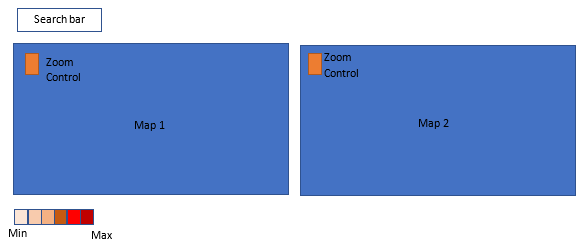
\includegraphics[width=.8\textwidth]{Pictures/FinalDesign}
	\caption{An illustration of the final design}
	\label{FinalDesignFig}
\end{figure}

The concept for a solution has been illustrated in figure \ref{FinalDesignFig}. The tool will use two maps with a shared view, so that both maps show the same area. Each map will show a different scenario, so that different population projections can be compared. Not all of the recommended functionalities presented in chapter x have been included in the design. Some of these functionalities will be mentioned in the discussion in chapter x.

\fxnote{Why does this not include everything mentioned in functions?}

\subsection{Visualisation}
The sequential color scale chosen for the visualized rasters have been created by colorbrewer.org. It was decided to use six different colors on the maps. This is despite the fact that \citet{ColorBrewerwebsite} advise that more colors safely can be used, when similar colors are neighboring each other. The reason for this is that even though similar colors are neighboring each other within the individual map, the user still has to compare none-neighboring colors, since comparison is done between the two maps. 
The breakpoints between the different classes are determined as percentage steps of 20 \% of the current maximum value. 
\fxnote{Why this projection? - vend tilbage efter carsten}

The mapped data is showing the population per square kilometre. It is therefore necessary that the area will not get distorted, so an equivalent projection is required. 

The equivalent projection EPSG:4326 was both used in Baumrocks original map and for the case data and will also be used for this project. 


\part{Development}
%In this chapter it is explained how the tool has been developed. The first section is describing the coding languages used and the plugins used to create the tool. The following sections are describing the necessary steps to build the tool. These steps can be seen in figure \ref{DevelopmentSteps}.

\begin{figure} [H]
	\centering
	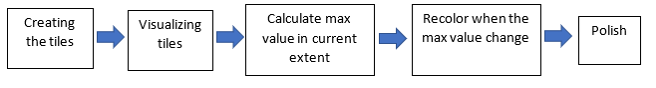
\includegraphics[width=.8\textwidth]{Pictures/DevelopmentSteps}
	\caption{An overview of the code}
	\label{DevelopmentSteps}
\end{figure}

First it is necessary to divide the raster into tiles to be able to limit the loaded data to the current extent. How this is done is explained in section x. Section x describes how the tiles have been visualized. To be able to color the tiles based on the current values it is required to know what the current values are. In section x it is explained how this information is calculated. The raster layer is then rerendered with these values as described in section x. Lastly some measurements were taken to ensure a more user-friendly experience. These additions are described in section x. 

\chapter{Coding languages and plugins}
For this project, the coding language Python was used to create the tiles, while visualization of the tiles was done in a webgis build with the languages HTML, CSS and Javascript. This webgis have been tested on a local caddy server for reasons explained in section x

\section{Languages}
\subsection*{Python}
Python is programming language with a simple syntax, which functions across multiple different platforms. This simple syntax means that Python can achieve the same as some other coding languages in fewer lines.\citep{WhatIsPython}
Python was used in this project because of the gdal library expanded further upon in section x
This project has been using version 3.6 of Python. 
\subsection*{HTML}
HTML is short for Hyper Text Markup Language. It is the language used for defining and structuring a web page’s content.
\subsection*{CSS}
CSS is an abbreviation for Cascading Style Sheets. This language defines how the HTML will be displayed.
\subsection*{Javascript}
How a webpage behaves is defined by the language Javascript.  This is what makes the web page interactive. 
\citep{WhatIsJs}

\section{Libraries}
To transform the raster data into smaller tiles the python library Gdal is used. 
\subsection*{Gdal}
GDAL is library for translating between multiple different geospatial data formats. \citep{GDAL} 

Included in this library is the gdal2tiles program, which can divide raster files into smaller tiles. 
At the time of using this program it was only able to generate tiles structured after the TMS standard. The function to follow the XYZ structure was added the 3th of May 2020 \citep{gdal2tilesDoc} \citep{GdalRelease}
%
The script rendering the tiles in the map was based on the XYZ structure. This meant that the rows of tiles were ordered incorrectly when the generated tiles were imported. Therefore, the official version of gdal2tiles was replaced by a version made by a github user named commenthol. This version is modified to allow the creation of tiles following the XYZ structure. \citep{gdalLeaflet}
Both the official version and the modified version have their output format as mbtiles with a bit depth of 8 bit. To be usable for this project a bit depth of at least 32 bit is needed, as mentioned in section x. The workaround for this issue will be explained in section x. 
\subsection*{Openlayers}
The map in which the tiles are being showed are created in Openlayers, which is an open source JavaScript library for creating dynamic maps for web pages. 
\citep{OL}
Openlayers was chosen because the tool presented in related work was built in Openlayers. Therefore, using Openlayers would enable expanding upon this existing tool instead of starting from scratch. 

The existing tool was created with the debug version of Openlayers, which this tool also have build on. The debug version is a version of the Openlayers, which have not been minified. Because of this it is a larger file than the regular one. 
https://gis.stackexchange.com/questions/155529/whats-difference-between-ol-js-and-ol-debug-js-files-in-openlayers-3
\fxnote{link}
Attempts at replacing it with the minified version resulted in errors from olGeoTiff, which have been build based on the debug version. Optimizing other parts of the code was given higher priority, so the debug version never got replaced. 

\subsection*{olGeoTiff}
olGeoTiff is a Javascript class for visualising geotiff tiles in Openlayers, utilising the libraries geotiff.js and Plotty. The visualized tiles are being processing in the client instead of on a server. It was used in the map presented in section x. 
The class is a modified version of Openlayers WMTS layer, where the internal tile loading function has been changed. The regular function would request precolored tiles and then add them to the map. The tiles requested by the modified version are not precolored and need to be processed before getting added to the map. A simplified illustration of this processing is illustrated in figure x. This simplified figure is enough to explain the mechanics of the class but does not detail the callback function structure. Aside from being used for error handling callbacks are also necessary to ensure that Openlayers do not try to add the tiles to the map, before they have been processed. More detailed figures can be found in \citep{Baumrocks} thesis.

\begin{figure} [H]
	\centering
	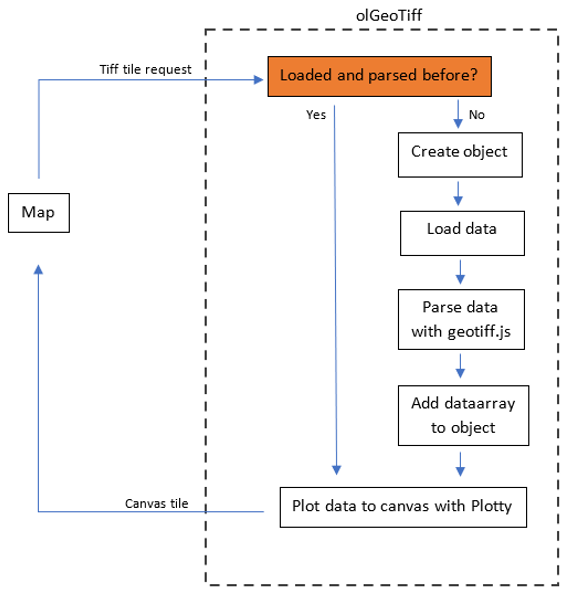
\includegraphics[width=.8\textwidth]{Pictures/olGeoTiffSimplified}
	\caption{A simplified illustration of how olGEoTiff functions}
	\label{olGeoTiffSimplified}
\end{figure}

To ensure that tiles are only being downloaded once an object keeps track of all the downloaded data. The object is organized by the tiles’ url. 
Whenever tiles are being requested the object will always be checked to see if it already contains the url. If it does not the object will be updated to include the requested tile. The tile will then be loaded before being processed. \citep{Baumrocks}
The processing is done with the TIFF parser geotiff.js 
\citep{Geotiff}
and Plotty, which is a library for creating images from data arrays \citep{Plotty}.

The loaded tiles first get parsed with geotiff.js and added to the object before Plotty get used to render tiles in the designated colors. Then the tiles get added to the map.
\citep{Baumrocks}
The olGeoTiff also have a redraw function, which when triggered will redraw the tile layer based on the current designated colors. This was for instance used in Bernnard Baumrocks map, whenever the color sliders were changed. 

\section{Testing server}
%Not finished 
To test the tool a local test server was set up. This was initially a Python-based http server, but was later replaced with a Go-based Caddy server to improve performance. The performance difference between the two is elaborated upon in section x.

Caddy was chosen because it supports the second version of Hyper Text Transfer Protocol (HTTP)
https://dassur.ma/things/h2setup/



which is used for the communication between the client and server.
https://www.w3schools.com/whatis/whatis_http.asp

HTTP/2 is allowing a faster communication between them
https://web.dev/uses-http2/?utm_source=lighthouse&utm_medium=devtools
%Caddy
%http’s limits to 6 connections 
%fig text: Blue: DomContentLoaded Red: Load
\chapter{Developing the tool}
This chapter details how the visualization tool was built.

\section{Creating the tiles}
The tiles were created using a modified version of gdal2tiles, which was changed to create tiles following the XYZ format. However, since the default output bit depth is too low, it would have to be modified further. The file format would also have to be changed to tiff in order to be visualized with the geotiff.js library. 

\subsection{Changing the file type}
Changing the file format can be done by changing two lines in the gdal2tiles script:

\begin{lstlisting}[language=iPython, caption={Changing the file format}, label= VoresPY,escapechar=|]
#Original code
#self.tiledriver = 'PNG'
#self.tileext = 'png'
#New code
self.tiledriver = 'GTiff'
self.tileext = 'tiff'
\end{lstlisting}
This changes the raster driver from png to the geotiff format and the file extension from png to tiff. 
\citep{RasterDrivers}
The geospatial information, which is the difference between a geotiff and a regular tiff, gets lost in process. This information is not important for this project since the tiles are being loaded based on their name and folder placement, not based on the internal metadata.

Running gdal2tiles with these changes will produce a tiff file, which still would be limited to 8 bits. 
\subsection{Increasing the bit depth}
The reason for the bit limit is that gdal2tiles uses the memory dataset driver, which have 8 bits as default.  This default can overwritten to 32 bits by adding “gdal.GDT\_Int32” to every instance where the driver is being used as demonstrated in code x. 
\citep{MoreThan8}

\begin{lstlisting}[language=iPython, caption={Increasing the bit depth}, label= VoresPY,escapechar=|]
self.mem_drv = gdal.GetDriverByName('MEM')
...
#Old code
#dstile = mem_drv.Create('', tile_size, tile_size, tilebands)
#New code
dstile = self.mem_drv.Create('', self.tilesize, self.tilesize, tilebands, gdal.GDT_Int32)
\end{lstlisting}
The memory driver is being used four times, which all have been changed in a similar fashion.


The script is now generating tiff tiles correctly. However it also generates KML files for visualization in Google Earth, which is undesired since it would increase the processing time and required storage space. 
\subsection{Prevent generation of Google Earth files}
gdal2tiles is automatically generating KML files if the projection is EPSG:4326. According to the documentation for the official gdal2tiles this can be disabled with the command "--no.kml".
\citep{gdal2tilesDoc}


This command does not prevent the creation of the files in the modified version. Therefore the automatic generation has been removed from the code. This was done by commenting out the lines shown in x. 

\begin{lstlisting}[language=iPython, caption={Increasing the bit depth}, label= KML,escapechar=|]
 if self.out_srs and srs4326.ExportToProj4() \
         == self.out_srs.ExportToProj4():
     self.kml = True
     self.isepsg4326 = True
     if self.options.verbose:
         print('KML autotest OK!')
\end{lstlisting}
        
\subsection{Command for tile creation}

After all the modification are in place the script can be run by running the command illustrated below:


python <path to modified gdal2tiles script> --leaflet --zoom=<desired zoom levels> --profile=raster --webviewer=none <input file> <output directory>


Most of these inputs are from the documentation for the original gdal2tiles, though the leaflet command is from the modified version. This command ensures that tiles are being created following the XYZ formatting instead of the TMS. The zoom command defines which zoom levels should be generated. An example of an input could be 0-2, which would generate tiles for the zoom levels 0, 1 and 2. 

Setting the profile to raster was done because the two other options (mercator and geodetic) resulted in the error message "list index out of range", while the raster profile gave a useable product. The selection of this options and its consequences is expanded upon in section x.  

The webviewer option prevent the generation of webviewers to visualize the tiles. These default webviewers is created to visualize tiles of the original format, so they would be unable to visualize the modified tiles. 
The input file is the name of the processed file and output directory is the folder, where the tiles get created. 
\subsection{Result}

While creating the tiles the error message "ERROR 1: Buffer too small" gets displayed. The tiles are still being generated with the correct formatting and bit depth. This is an error message from numpy, which gdal2tiles are using. 
\citep{MoreThan8}
The generated tiles appears as they should, so this error message is potentially referring to the geospatial information, which gets lost.

%The tiles at the rightmost and bottom edges have an edge as shown in figure x. This edge is not being shown, when the tile is being loaded into the map. A comparison between the input file and the tile shows that all data is being displayed. The bottom part of the input file is the last part before the edge. This edge seems to be generated because the input file was not perfectly dividable with the tile size as illustrated in figure x.
%https://github.com/ARiisgaard/Thesis/issues/22
%This edge could be another explanation for the error message. 

The script also produces an xml file with metadata. An example of the content of said metadata file can be seen in code \ref{metaData}.

\begin{lstlisting}[language=HTML5, caption={The metadata from the xml file generated by the modified gdal2tiles}, label= metaData,escapechar=|]
<?xml version="1.0" encoding="UTF-8"?>
<TileMap tilemapservice="http://tms.osgeo.org/1.0.0" version="1.0.0"><Abstract/><SRS>GEOGCS["WGS 84",DATUM["WGS_1984",SPHEROID["WGS 84",6378137,298.257223563,AUTHORITY["EPSG","7030"]],
AUTHORITY["EPSG","6326"]],PRIMEM["Greenwich",0,AUTHORITY["EPSG","8901"]],UNIT["degree",0.0174532925199433,
AUTHORITY["EPSG","9122"]],AXIS["Latitude",NORTH],AXIS["Longitude",EAST],AUTHORITY["EPSG","4326"]]
</SRS><BoundingBox maxy="25.00000000000814" maxx="80.99999999999989" miny="19.00000000000815" minx="72.99999999999989"/><Origin y="19.00000000000815" x="72.99999999999989"/><TileFormat extension="tiff" mime-type="image/tiff" height="256" width="256"/><TileSets profile="raster"><TileSet order="2" units-per-pixel="0.00833333333333" href="2"/><TileSet order="3" units-per-pixel="0.00416666666667" href="3"/><TileSet order="4" units-per-pixel="0.00208333333333" href="4"/><TileSet order="5" units-per-pixel="0.00104166666667" href="5"/><TileSet order="6" units-per-pixel="0.00052083333333" href="6"/><TileSet order="7" units-per-pixel="0.00026041666667" href="7"/><TileSet order="8" units-per-pixel="0.00013020833333" href="8"/><TileSet order="9" units-per-pixel="0.00006510416667" href="9"/></TileSets></TileMap>
\end{lstlisting}

\section{Processing time}\label{TilesTime}

\begin{figure} [H]
	\centering
	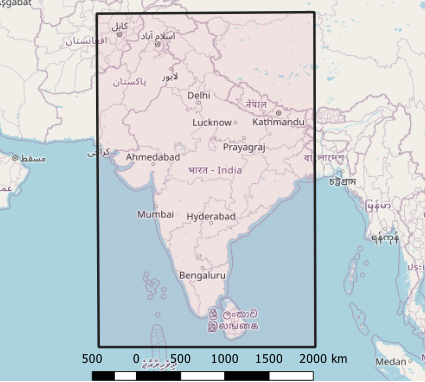
\includegraphics[width=.6\textwidth]{Pictures/ProcessingTime}
	\caption{Illustration of the area used for timing the tile generation}
	\label{ProcessingTime}
\end{figure}

The processing time is tested using the area of India shown in figure \citep{ProcessingTime}. This polygon with a 9 291 842 km$^2$ area was processed into tiles for each zoom level between 0 to 9. This is the equivalent of 349525 tiles as calculated with the formula presented in section x. 
\begin{equation}
2^{2n}
2^{2*9}+2^{2*8} .. . 2^{2*0} = 349525 tiles
\end{equation}
The creation of these tiles took 6 hours and 4 minutes and requires 6,52 GB of diskspace The amount of time mainly depends on the highest zoom level, since the number of tiles in a layer get quadrupled whenever the zoom level increases. In comparison the same area at the zoom levels 0-7 only took 22 minutes.

This processing time is not ideal, but it can theoretically be shortened with multiprocessing.
\subsection{Parallel processing of tiles}
Multiprocessing is the usage of multiple of the computer’s processors. Python is by default only able to use a single processor, even if multiple are available.  This can be circumvented with the multiprocessing module.
%Must not be reliant on previous outcomes
%Does not need to be executed in a particular order
%Does not return anything that would need to be accessed later in the code
\citep{Multiprocessing}
The modified version by \citet{gdalLeaflet} also has a multiprocessing version allowing each processer of the computer to work separately on generating tiles. However, the task is not properly distributed between the processes. This means that not all of the tiles are being generated. 
\citep{NoMulti}
Therefore, the slower single process version has been used for this project.


\section{Visualizing tiles}
After the tiles are created, they are stored in a folder, which is uploaded to the testserver along the index file. 
The metadata from the xml file must be loaded into the map to be able to visualize the tiles. Normally this could be done using the WMTSCapabilities() function in Openlayers.
\citep{WmtsOl}
However, the formatting of the xml file produced by gdal is different from the format, which this function can read. Therefore, a small script has been created to parse the xml file and store the information in a metadata object. This object, tileMetadata, stores the bounding box, origin, center coordinates as well as tilesize. The initial version of the object also stored the resolution data, which is called units-per-pixel in code x. This led to some inconsistency when loading tiles, that had been generated without some of the lower zoom level. This will be further expanded upon in section x. Therefore, the resolution was instead generated using the script x, where 0.0333 is the value for units-per-pixel at zoom level 0. 

\begin{lstlisting}[language=JavaScript, caption={The JavaScript in the project}, label= VoresJS,escapechar=|]
for (var z = 0; z < 14; ++z) {
// generate resolutions and matrixIds arrays for this WMTS
//The number in the resolution calculation is the units-per-pixel value at zoomlayer 0 in the xml file generated by gdal2tiles
resolutions[z] = 0.03333333333514 / Math.pow(2, z);
matrixIds[z] = z;
}
\end{lstlisting}
Using this metadata, the tiles could be visualized using the olGeoTiff class. 

%\begin{lstlisting}[language=JavaScript, caption={The JavaScript in the project}, label= VoresJS,escapechar=|]
%var wmslayer = new ol.layer.Tile({
%  source: new ol.source.WMTS({
%    url: tileFolders + '/{TileMatrix}/{TileCol}/{TileRow}.tiff',
%    projection: projection,
%    tileGrid: new ol.tilegrid.WMTS({
%      origin: tileMetadata[origin],
%      resolutions: resolutions,
%      matrixIds: matrixIds,
%      tileSize: tileMetadata[tileSize],
%    }),
%    requestEncoding: 'REST',
%    transition: 0
%  }),
%  extent: tileMetadata[boundingBox],
%  opacity: 0.65 
%});
%var olgt_map = new olGeoTiff(wmslayer);
%\end{lstlisting}


\subsection{Custom colors scheme}
Using colorbrewer a custom sequential colorscheme was generated. This scheme was added to Plotty and selected as a color palette. 

\begin{figure} [H]
	\centering
	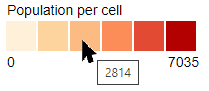
\includegraphics[width=.4\textwidth]{Pictures/CScale}
	\caption{The scale added to the map. When mousing over a color, the assigned value is displayed}
	\label{CScale}
\end{figure}

The value assigned to each color can be found by mousing over the color as shown in figure \ref{CScale}


\section{Loading data at a wrong resolution}\label{PresentingBug}

Figure \ref{MapWithWrongResolution} shows how the map looked, when the tiles are visualized. 
\fxnote{Rewrite this with new knowledge}

\begin{figure} [H]
	\centering
	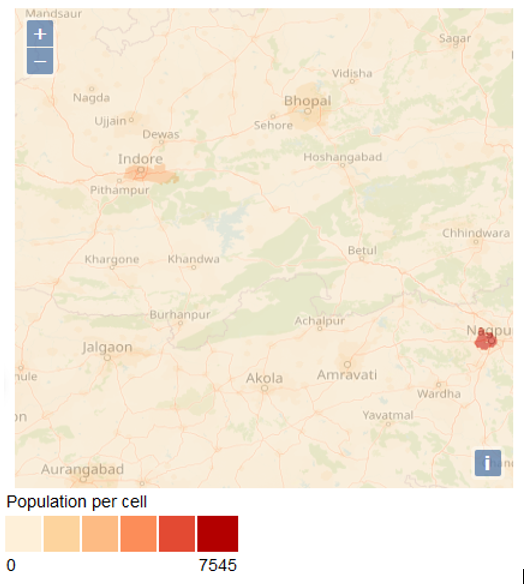
\includegraphics[width=.6\textwidth]{Pictures/MapWithWrongResolution}
	\caption{The map is looking correct, but with tiles from the wrong zoom level}
	\label{MapWithWrongResolution}
\end{figure}


While the map appeared to look alright, it was loading tiles from the wrong zoom level. The tiles always got loaded from a zoom level three levels higher than intended. So the map in figure \ref{MapWithWrongResolution} is visualizing the map at zoom level 7, but loading and displaying tiles from zoom level 2. It was not possible to force the map to load tiles from a different zoom level.

Some experiments with loading tiles from the current view and zoom level 7 crashed the map with the error message “Insufficient Resources”. The amount of loaded tiles seems unnecessarily high and size of the tiles too small. This seems to indicate, that the tiles, which the modified version of gdal2tiles associates with zoom level 7 in fact belongs to a higher zoom level.

In figure \ref{DifferentZoom} these different zoom levels have been illustrated. The expected zoom level, which Openlayer

The Displayed zoom level (DZL) is the tiles, that are being loaded and visualised in Openlayers. The expected zoom level (EZL) is the zoom level, which Openlayers is displaying the map in. However as mentioned earlier there are too many tiles to load, when using this zoom level and map extent. The coloring should therefore ideally be done based on a zoom level between these two zoom levels. This zoom level have been defined as the intended zoom level (IZL).

\begin{figure} [H]
	\centering
	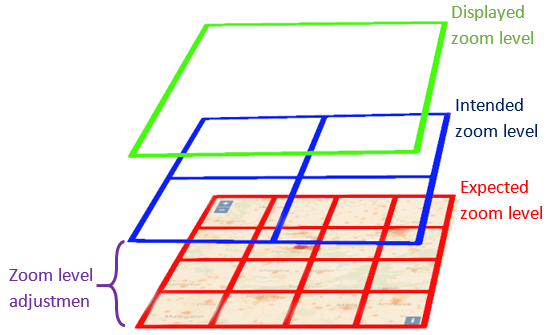
\includegraphics[width=.6\textwidth]{Pictures/DifferentZoom}
	\caption{An overview of the differences in zoom levels, which the map is displayed at (red), the displayed tiles get loaded in (green) and the zoom level, which should have been displayed (blue). The zoom level adjustment is the difference between the Expected and Intended zoom level}
	\label{DifferentZoom}
\end{figure}
\fxnote{Explain the need for zoom level 0 better}
This issue was not fixed, but theories behind the origin of it is discussed in section x. When the resolution data was gathered from the metadata file, the difference between the loaded and the actual zoom level would between different sets of tiles. This variance would depend on the which zoom levels were not being generated. So, if only the zoom levels 2-7 were generated, the difference would increase by one for each missing layer. In this case the loaded tiles would instead be wrong by 5, calculated as the default wrongness of 3 plus 2 for missing zoom layer 0 and 1. 
This bug will be defining for the rest of the code.



\section{Calculate max value in current extent}
Calculating the highest value in the current extent can be divided into two smaller tasks. Figuring out which tiles currently are being displayed and processing these tiles. It was decided not to calculate the lowest value in each tiles, since the calculation increased the processing time without yielding any benefit. This is expanded upon in section \ref{WhyNoMin}

\fxnote{min values have been removed earlier, right? No need to mention them here too}
\subsection{Current displayed tiles}\label{CurrentDisplayedTiles}

The tiles, which currently is within the view, can be found using the Openlayers tileGrid method forEachTileCoord. This method can trigger a function for each tile coordinate within a given zoom level and extent. 
\citep{forEachTileCoord}
These tile coordinates can then be translated to the tile name and folder location using getTileUrlFunction.
%The method is going through the tiles based on their coordinates, but this can be translated to the tile urls using the getTileUrlFunction.
\begin{lstlisting}[language=JavaScript, caption={}, label= VoresJS,escapechar=|]
var tileUrlFunction = wmslayer.getSource().getTileUrlFunction()
var zoomlevelAdjustment = 3
wmslayer.getSource().getTileGrid().forEachTileCoord(loadExtent, mapZoom - zoomlevelAdjustment, function(tileCoord) {
	tileName = tileUrlFunction(tileCoord, ol.proj.get('EPSG:4326'))
	maxValueInTile()
}
\end{lstlisting}
If the function is just given the zoom level of the map it will trigger for the tiles in the Expected Zoom Level. This would not work, since there are too many tiles in this level with the current extent. Instead the function is used with the Intended Zoom Level, which is calculated as the Expected Zoom Level minus a zoom level adjustment. Using an adjustment value of 3 was found to give a responsive user experience.

% This means that it on zoom level 7 would load the tiles, that should be rendered on zoom level 7. Due to the issue mentioned section \ref{PresentingBug} it is not the tiles from that zoom level, which are being displayed. Instead the tiles from zoom level 2 are being displayed. This will complicate some of the next steps. 
%The adjustment to the zoom level is in order to load the tiles, which should have been displayed.

\subsection{Max value for each tile}
If the tiles added to the map had been from the Intended Zoom Level, then the max value of a tile could have been calculated as olGeoTiff was running. olGeoTiff already holds the values for the tiles in a dataarray, so finding the maximum value could be done with a single line adding a tiles max value to the object for that tile. %This line is shown in code x, where urlToTiff is the name of the object, which holds the data.

%maxValueTileData[url].maxValue = Math.max(...urlToTiff[url][0])

However, since olGeoTiff holds data from an incorrect zoom layer this does not function. A possible solution would be to trigger forEachTileCoord for the Displayed Zoom Level. This solution was not implemented since the tiles from the Displayed Zoom Level are so large, that they would show data outside the view of the map. This means that the coloring could be based on the information that was outside of the current view.

The alternative solution is to run another function going through the tiles, which should have been displayed and find the highest value among these. This results in a map where the tiles from the Displayed zoom level were being colored based on information from the tiles at the Intended zoom level. This solution is by no means ideal. It means requesting tiles from two layers, one for displaying on the map a one for calculating the relevant max values. Loading more data than necessary will make the script slower, but since no better solution was found this have been implemented.

The calculation of the maximum value for each tile was done in a very similar fashion to how olGeoTiff operates as illustrated in figure \ref{CalculateMaxValue}. An object holds information about all tiles, which have been processed and the max value is known. When the function is run for a tile it first checks if the tile already has been processed. If that is not the case, then it will create an object for the data, which it then will load and parse with geotiff.js. %The data array with parsed data will then be run through as descripted in code x to calculate the maximum value. 
This maximum value will then be returned to the map. 

\fxnote{Write about combining my object with his object - would result in it not having to open the same raster twice, in case of zooming}
\begin{figure} [H]
	\centering
	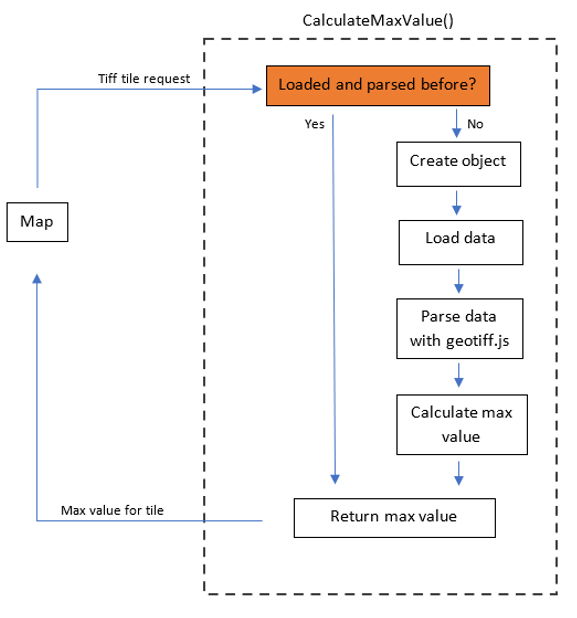
\includegraphics[width=.6\textwidth]{Pictures/CalculateMaxValue}
	\caption{Flow diagram of the calculation over max value in a tile}
	\label{CalculateMaxValue}
\end{figure}



\subsection{Highest tile value currently displayed}


To find the largest tile value among all the currently displayed tiles forEachTileCoord is used. forEachTileCoord does not have a trigger for when it has run through all the tiles. This functionality is necessary for ensuring that the produced maximum value is actually the maximum value. Without a precise end trigger the coloring applied to the map could be based on the biggest value found before the coloring script stated running instead of the absolute highest value in the current display.
Since this trigger is necessary it has been created by running forEachTileCoord another time to count the number of tiles. This part of the code can be seen in code \ref{TilesInExtent}.
\begin{lstlisting}[language=JavaScript, caption={Counting the amount of tiles within the current extent}, label= TilesInExtent,escapechar=|] 
var tileNumber = 0;
wmslayerMap1.getSource().getTileGrid().forEachTileCoord(loadExtent, mapZoom - zoomlevelAdjustment, function(tileCoord) {
	tileNumber++;
})
\end{lstlisting}
The recoloring of the map can then be delayed until the function for calculating the maximum value have been running for the same amount of times as there are tiles on the map. In practical terms this can be accomplished by adding a counter and an if statement to the maximum-value-function. The counter would check how many times the function has run. The if statement would check if the amount of times the function had been run was equal to the number of tiles. If this is the case and the registered max value is different from the previous one the recolor function would trigger.
The calculation of the maximum value is the function presented in figure \ref{DoubleLoop}. It is running asynchronously because the array otherwise would be filled with “undefined” values instead of actual values. Running it asynchronously ensures that the script awaits the calculation of the value.  
\begin{figure} [H]
	\centering
	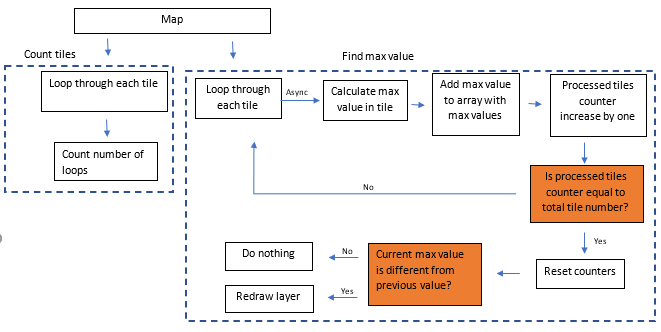
\includegraphics[width=1\textwidth]{Pictures/DoubleLoop}
	\caption{Finding the largest value in all currently displayed tiles}
	\label{DoubleLoop}
\end{figure}

\section{Recolor when the max value change}

The recoloring function was already part of olGeoTiff. However, in Bernhard Baumrocks’ thesis this recoloring was triggered manually by the user when changing the color sliders. In this project the changing of colors will trigger automatically. The function for recoloring the map have therefore been set up to trigger, when the user stops changing the view. By not triggering before the map movement is finished a smoother user experience is ensured, since new tiles does not have to processed before the user is finished with interacting with the map. The recolor function is running through all of the code mentioned in the previous sections. 

\begin{lstlisting}[language=JavaScript, caption={The JavaScript in the project}, label= VoresJS,escapechar=|]
map.on("moveend", function() {
recolorMap()
});
});
\end{lstlisting}
\section{Polish}
In addition to the rendering of the raster in the map, some features were also added to improve the user experience.

\fxnote{Nævner jeg tileMetadata?}
\subsection{Two maps}\label{DTTwoMaps}

\begin{figure} [H]
	\centering
	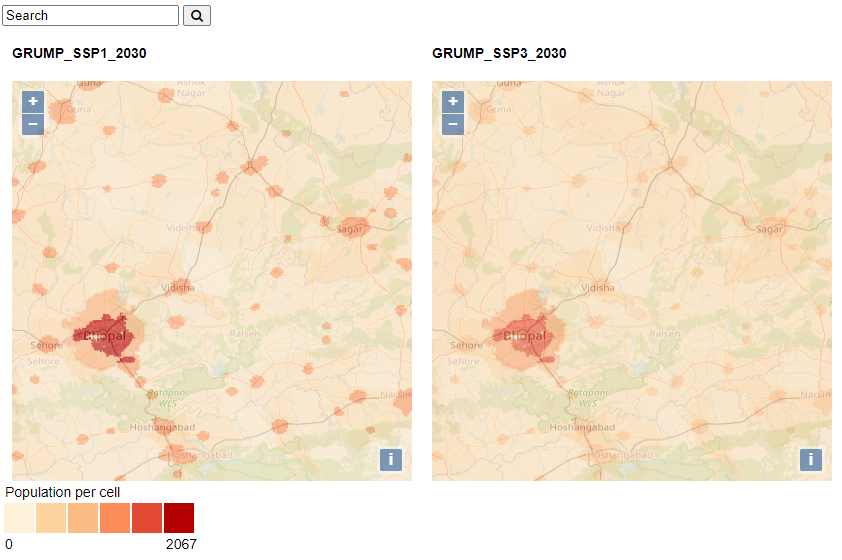
\includegraphics[width=.8\textwidth]{Pictures/Frontpage}
	\caption{A second map beside the first one. Each map is showing a different dataset as shown above the maps}
	\label{DualMaps}
\end{figure}

To be able to compare different rasters with each other a second map was added as illustrated in figure \ref{DualMaps}. This second map is having its own raster dataset but sharing the view with the first map. This means that the two maps would always show the same area. Panning or zooming in one map would do the same action in the other map. The two maps are sharing the same legend. Above each map is the name of the dataset, which is shown in the map.  

The two projection are also sharing the same color scale. This means that the coloring is done based on the maximum value in the current extent of either of the maps. To accomplish this changes were made to the function, which were finding the maximum value among the tiles as illustrated in figure \ref{ChangeToMaxCalculation}.
 
\begin{figure} [H]
	\centering
	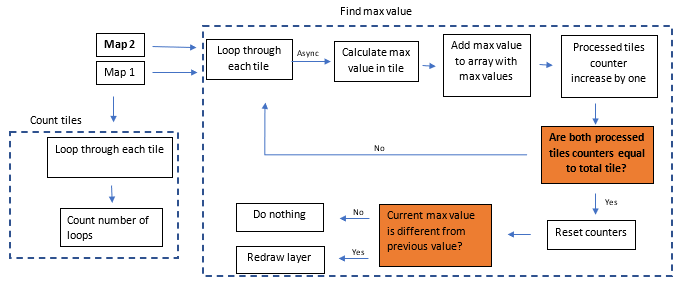
\includegraphics[width=1\textwidth]{Pictures/ChangeToMaxCalculation}
	\caption{Calculating the maximum value for two maps. Changes from the original have been written in bold}
	\label{ChangeToMaxCalculation}
\end{figure}

This function is now being used twice, once for each layer. If the same function as presented in section x was used, then the redrawing would potentially trigger twice. 

To avoid this each of the maps are given their own processed tiles counter. The if statement, which is resetting the counters and triggering the recoloring, has been changed, so that it now is checking if both of these processed tiles counters is equal to the total number of tiles. Thereby the recoloring can only happen, when the tile in both maps have been processed. 

The two maps would always display the same amount of tiles, since they are sharing the same view. It is therefore only necessary to calculate the amount of tiles for one of the layers. 
%Add to dualmaps how the double evaluation for multiple maps were build 

The size of the maps were set to 400x400 pixels, which did not take up the full width of the page. This was done for both a performance and a scientific reason. From a performance perspective a small map requires less tiles and is therefore faster to loaded. Decreasing the width from using the full extent of the screen (700 pixels per map) improved the initial loading time from 5.31 seconds to 3.61 seconds. The measurement of performance is further elaborated in chapter \ref{EvalMethods}. 
The scientific reason is consistency in performance measurements. By having a fixed size, there would be no difference between measurement due to differences in screen size. How the empty space next to the maps could be utilised is described in section \ref{MoreInfoPlz}.  
 

\subsection{Search function}
In order to be able to faster navigate the map a search function was created as shown in figure \ref{SearchBar}. 

\begin{figure} [H]
	\centering
	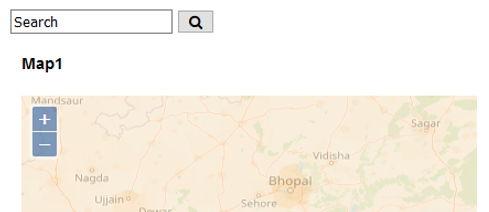
\includegraphics[width=.6\textwidth]{Pictures/SearchBar}
	\caption{The map can pan to a specific area, by searching for that area in the searchbar}
	\label{SearchBar}
\end{figure}

The user can use this to change the current view of the maps to a given location. This is accomplished through the help of Nominatim. This tool can search through Openstreetmap data by location names. It then returns data about the searched location. 

Among this data is the latitude and longitude for the central point of the place. \citep{Nominatim}
This coordinate is then used as the coordinate for the center of the map.

\section{Final product}

This section is an overview of the final product, which can be seen in figure \ref{FinalProduct}. 
The datasets highlighted in the figure is elaborated upon in section \ref{Comparisons}.


\begin{figure} [H]
	\centering
	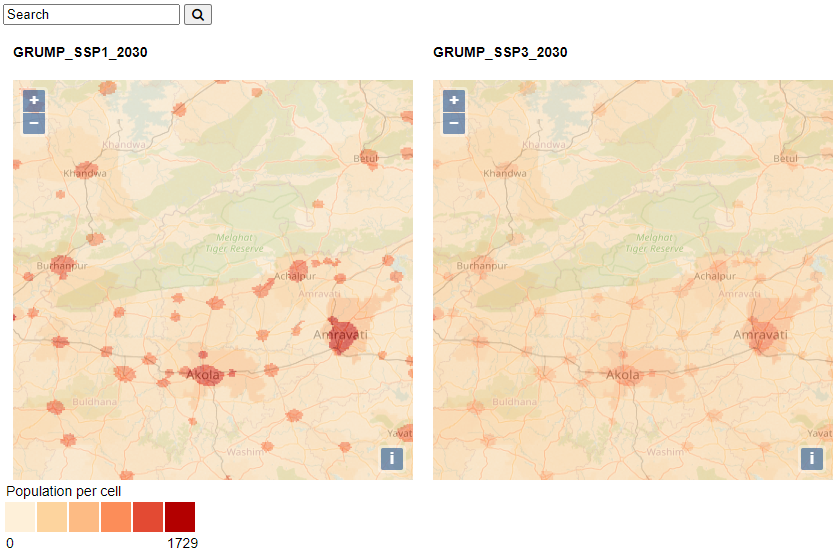
\includegraphics[width=.8\textwidth]{Pictures/FinalProduct}
	\caption{The final product}
	\label{FinalProduct}
\end{figure}

The main part of the final product is two maps, which are showing two different scenarios for the future. These maps have the same color scale and are always showing the same extent. The values in this color scale are automaticity updated to reflect the highest value within the current extent. The user can see which values the colors are assigned by mousing over the colors. 

Above the two maps are the names of the datasets, which currently are being displayed. Above these names is a search bar, which can be used to pan to a searched location.  
\fxnote{Har jeg skrevet om at score bliver udregnet ud fra en sammenligning med fulde hjemmesider}
\section{Comparisons}\label{Comparisons}
\fxnote{Consistent omkring lighthouse}
This section highlights comparisons between different scenarios. 

The datasets, which were displayed in figure \ref{FinalProduct} are SSP1 and SSP3 with GRUMP as urbanisation definition and year 2030. These two scenarios have been chosen, because of their differences as mentioned in section \ref{SSPs}. The first scenario have a low population growth and fast urbanisation rate, whereas the other have a high population growth and slow urbanisation rate. This leads to areas with higher density in the SSP1 scenario, even though there is a bigger population in the SP3 scenario. The faster urbanisation means that this larger population gets spread over a larger area, which lowers the density.

\begin{figure} [H]
	\centering
	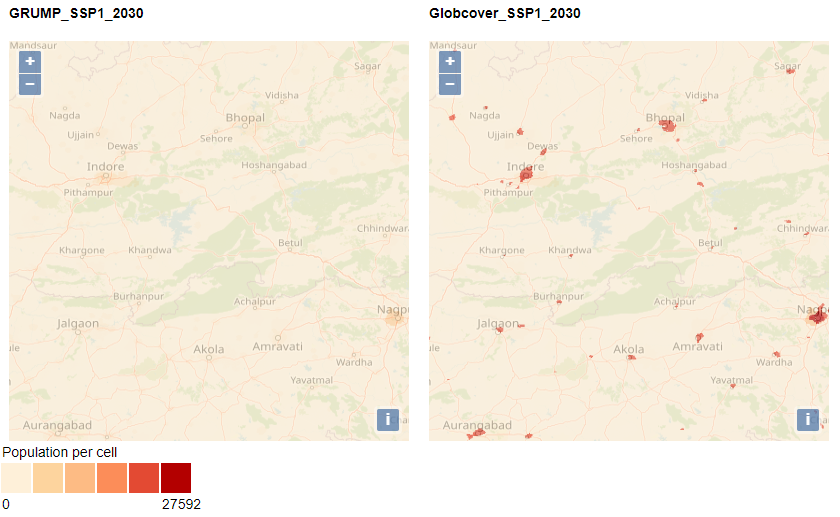
\includegraphics[width=.8\textwidth]{Pictures/GlobcoverVsGrump}
	\caption{A comparison between different urbanisation definitions with the same scenario and year}
	\label{GlobcoverVsGrump}
\end{figure}

Figure \ref{GlobcoverVsGrump} shows the difference between the urbanisation definitions. The urban density in much higher, when using the GlobCover definition (right) compared with the GRUMP definition (left). This is due to the fact that both models have the same amount of people living in urban environments, but GRUMP overestimates the urban areas as mentioned in section \ref{TheDataBehind}.  

This mean that a geosimulation with GlobCover as urban definition has smaller areas to squeeze the same population into, which leads to higher densities in the cities.


%\chapter{Result}

here is a map of the end result and writting about what it can do

\part{ Evaluation}
\chapter{Evaluation Methods}

In this chapter the methods for evaluating the product will be presented.


Due to the limitations mentioned in section \ref{Lim} user testing was not a possibility. This meant that it was necessary to find another way to evaluate the user experience. This was done using Google Lighthouse version 5.7. 
This chapter starts with an overview of the tool followed by an evaluation of which criteria are relevant for this project. The relevant criteria and their metrics are then expanded upon.

\section{Setup}


The tests have been performed in Google Chrome version 81. To ensure that tests were unaffected by outside influences all Chrome extensions were disabled during testing. The Cache


\section{Overview}
Google Lighthouse is an automated tool in Chrome DevTools, which is the developer tool included in Chrome. It can be used to check the quality of websites within the five categories: Best practice, performance, accessibility, search engine optimization and progressive web app. \citep{Lighthouse}
\fxnote{Inset Image here}

\textbf{Performance}\\
The performance audit is measuring the site performance and load speed. This is done by measuring the time needed for different stages of loading and when the user is able to interact with the site. \citep{LhPerformance}


\textbf{Accessibility}\\
The accessibility check is for ensuring all users can effectively access and navigate the webpage. 
The check is mainly focused on Accessible Rich Internet Applications, which is used by assistive technologies such as screen readers.\citep{ARIA} It is pointed out that accessibility is difficult to automatically test, so further manual testing is recommended. 

\citep{LhAccess}

\textbf{Best practice}\\
The best practices cover different types of website enhancements. There checks to ensure that the website is fast, secure, and not using deprecated technologies, among others. \citep{LhBP}

\textbf{Search engine optimization}\\
The checks within the Search Engine Optimization (SEO) category evaluate how well the page is optimized for ranking by search engine. This optimization is achieved by ensuring that the page is readable search engines and that search engines can access the page. It also includes some measurements for being mobile friendly.
\citep{LhSEO}

\textbf{Progressive web app}\\
The Progressive Web App (PWA) audits are target towards a mobile audience. These includes having a fast and reliable experience on mobile networks and to which degree the website act in a similar fashion to a native mobile application.
\citep{LhPWA}

\subsection{Relevant evaluation criteria}
 
Not all the audit categories in Google Lighthouse are relevant for this particular project. As mentioned in section \ref{Target audience}  the tool is developed for local use on a computer. This means that it is not relevant how optimized a site is for the phone. Since it is used locally it can not be found by a search engine, which makes the SEO category irrelevant. The best practices for enhancing the websites speed are relevant, while the security measures are not, since the tool is not accessible to others on the internet. While accessibility is important it has not been prioritised for the development of this prototype. The main argument is that the tool is being developed for data scientist and not for anybody. It is presumed that the majority of people, who daily work with computers have the sensory capacity to easily do so. A high performance is vital to ensuring a responsive user experience, so the performance audit will also be included.

\fxnote{Write target audience}


\section{Metrics for performance}

\fxnote{Write about timing the python processing}


\fxnote{Source: Return to this one later}


\textbf{First Contentful Paint}

The First Contentful Paint (FCP) is the time in seconds it takes before the browser to render the first parts of the website. 
\citep{FCP}


\textbf{Speed Index}

The Speed Index (SI) is a time measurement of content appearing visually during load. To calculate it the visual progression between each frame of the loading process is measured. This is then being processed using the Speedline module. The unit is seconds. \citep{PerSI}

The Speedline module calculates the SI by calculating an Interval Score between each frame and then summaries all the Interval Scores. The Interval Score can be calculated using the formula \ref{SIFormula}, where the Interval is the elapsed time since last frame and Completeness is the percentage of visual completeness. \citep{SIformula}
\begin{equation}
 IntervalScore = Interval * \left( 1.0 - \frac{Completeness}{100} \right)
\end{equation}\label{SIFormula}


\textbf{First Meaningful Paint}

The First Meaningful Paint (FMP) is the seconds from the initial loading of the page to the primary content is visible. Where primary content is referring to the largest layout change, which is visible without scrolling.

It should be noted that FMP is being replaced with Largest Contentful Paint (LCP) in the next release of Chrome Lighthouse. The reason for this is that FMP is did not give consistent result and was difficult to standardize in all web browsers. \citep{FMP}
LCP is the seconds needed to render the single largest content element, which is visible without scrolling.\citep{LCP}

\textbf{Time to Interactive}

The Time to Interactive (TTI) is the seconds before a loaded website is completely interactive. This time is defined as after FCP when most of visible elements can be interacted with and respond within 50 milliseconds. 
\citep{TTI}

\textbf{First CPU Idle}

First CPU Idle is the seconds before a page becomes minimally interactive. Minimally interactive is defined as when the majority of the visible User Interface elements are interactive and giving responds within a reasonable time. 
The difference between this and TTI is the degree of interaction. When the user can begin interacting with a page the First CPU Idle can be measured. TTI is measured when all interactions can be performed. 
This feature is being replaced with Total Blocking Time (TBT) in the next Lighthouse release. The reason for this is that this and TTI are too similar to maintain both. 
\citep{FCPUI}
TBT is the total amount of milliseconds where the website is not responding to user input. It is measured during the time between FCP and TTI. 
\citep{TBT}

\section{Calculating score}

Each of the metrics in the section above are then converted into a score between 0 and 100. This score is calculated by comparing each metric with performance data from real websites in the HTTP Archive.
https://web.dev/performance-scoring/
The scores from each metrics are then weighted to reflect that each factor does not have the same importance for the perceived performance. The weight of each metric can be seen in table x.

\fxnote{Make table with score weights}

\section{Additional measurements}

The measurement mentioned so far only take the initial load into consideration, not the postload performance. 
Therefore, two additional measurements were conducted. Both of these were measured using the Performance tool in the Google Chrome Developer tool. Since there are slight variation in the time needed to perform the requests, each operation was tested multiple time and the average was calculated. 
\subsection{Time to color new layer}
This is the time in seconds required to load and color completely new sets of tiles for both maps. The scenario is created by zooming to a new zoom extent. This is done to ensure that none of the tiles on the map have been loaded before. The measured time is the time from the map is clicked, initiating the zooming, till the layer have been colored.

\subsection{Time to recolor a loaded layer}
This measurement is the time recolor a layer with loading. This scenario is created by panning to a previously loaded part of the map, so that it is recolored.
It is measured from the moment, the panning stops since the recoloring script is initiated on ended movement. The timer is stopped, when the layer is recolored.


\chapter{Evaluation}
This chapter is the evaluation of the script based on the Google Lighthouse audit. This chapter will highlight some elements of the audit. The full audit can be seen in appendix x. The given score in the relevant categories can be seen in figure x. There was a bug in the measurement of the performance score, which will be further expanded upon in section x. This means that the tool. It does however still provide some useful suggestions as to how the site could be improved.




\begin{figure} [H]
	\centering
	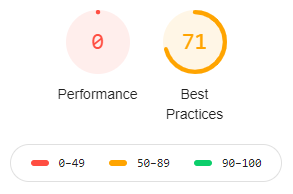
\includegraphics[width=.8\textwidth]{Pictures/LighthouseGrade}
	\caption{The score for performance and best pratices from Google Lighthouse}
	\label{LighthouseGrade}
\end{figure}

\subsection{Performance}
As shown the performance scored nothing out of a hundred. The performance in each of the metrics can be seen in figure x.

\begin{figure} [H]
	\centering
	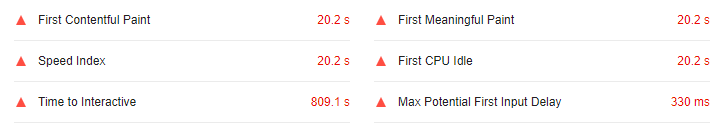
\includegraphics[width=.8\textwidth]{Pictures/PerformanceAuditValues}
	\caption{The result of the performance audit}
	\label{PerformanceAuditValues}
\end{figure}

\fxnote{Write that it is nonsense}

\subsection{Opportunities}
In addition to providing the metrics for the performance Lighthouse also comes with suggestion to how the loading time can be reduced. 
\textbf{Eliminate render-blocking resources}
The opportunity for the largest estimated time saving is to eliminate render-blocking resources. These are the URLs, which must be loaded before the first paint can be applied to the page. \citep{RenderBlocking}

Table x shows the different libraries, which have to be loaded before the site is rendered. It can be seen that Openlayers is 82 \% of the loaded data.
\fxnote{Have I written about Jquery??}

\begin{table}[htbp]
	\centering
	\begin{tabular}{l}
		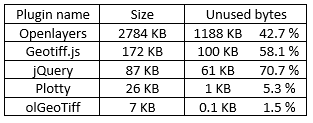
\includegraphics[width=0.8\textwidth]{Pictures/tabPluginSize}
	\end{tabular}
	\caption{Size of loaded modules and the much they are used}
	\label{tabPluginSize}
\end{table}

When analysed further with the Coverage tool it can be seen that a large part of the Openlayers library is not being used as show in table \ref{tabPluginSize}.  
\fxnote{TODO: Make a table from the information in the figure below – tabtext – resourse use of the 3 larges libraries}

\fxnote{Write about Coverage earlier – maybe in evaluation tools}

\textbf{Minification and compressing}
Files sizes and script parsing time can be reduced by minifying and compressing the files. 

A minified file is a file, where all the unnecessary parts have been cut away. Whitespaces and unused code are removed leaving a smaller file, which still functions perfectly. 

Compression is using an algorithm to modify the data, so that it takes up less space.
\citep{MinifyJS}
\fxnote{For exam: Try using Terser to minify and compress – Write about Terser in future work}
\textbf{Avoid enormous network payloads}
Long loading times are highly correlated with the amount of loaded data.  
\citep{LoadingTooMuch}

Loading the raster tiles for the map does require loading multiple files with a large bit depth, which requires a lengthy loading time. 

\textbf{Does not use HTTP/2 for all of its resources}
This suggested improvement appears if some of the page’s resources are being served with a version of HTTP/1. According to Google Audit all loaded resources are being delivered using HTTP 1.1.

\fxnote{Write about HTTP/2 earlier?}

\citep{HTTP2}

\textbf{Uses deprecated APIs}
When loading the metadata about the tiles a synchronous XMLRequest is used. This is a deprecated API, which will be removed from Chrome in a feature edition. 
\citep{OldApis}

\chapter{Discussion}

\fxnote{Write about smaller maps for better performance }
\fxnote{Update final design to not have scale}

\section{Loading tiles from the wrong zoom level}

As mentioned in section x the tiles are being loaded from an incorrect zoom layer. A potential explanation for this could be the difference between what gdal2tiles and Openlayers define as zoom level 0. Openlayers defines zoom level 0 as the whole world, whereas gdal2tiles defines it as the whole raster. 

It was discovered that the tile from zoom level 0 would be rendered in Openlayers, when the entirety of the raster was visible. This means that if tiles were generated for the entire world, then the zoom levels would be the same. 

The tiles could possibly be ordered and named correctly by running gdal2tiles with a different profile.  It was originally run with the raster profile, because the other profiles resulted in an error message as mentioned in section x. 


\section{Further development}
Not all the intended functionality got added to the map. This section will list some of the features, which there was not time to implement. 

%\subsection{Data at point of click}
%
%A function could be added to get the population counts from a clicked point for both maps. An example of this have been shown in figure x. When the user clicks the map an infobox informs the user about the value at the clicked point for both maps. 
%TODO: Figure showing a popup on click
%-	Popup text: Data in this map and data in the other





\subsection{Changing layers}
Another functionality, which could have been added was the option to change the datasets of the maps. As mentioned in section x the case data contains population projection for ten different years. It does therefore make sense to have the option display more than the two datasets.  As illustrated in figure x data from other years could be added as separate layers. This would allow the user to compare different datasets without having to reload the webgis with different datasets.

This way the map could also be used to visualize the different in the same projection from one year and another.
\subsection{Option for multiple colorschemes}
If there is a vast difference between the values in the two shown projection coloring based on the same maximum values does not necessarily make sense as was shown in the figure in core concept 2. It would therefore make sense to have the option to enable separate coloring as shown in figure x. 
TODO: make a figure showing the map with multiple legends and color schemes. 

\subsection{Additional information}

Currently the user can not get exact information about the the population density at a given point. They know the approximate value because of the legend, but not the exact value. 

A function could be added to get the population counts from a clicked point for both maps. When the user clicks the map an infobox informs the user about the value at the clicked point for both maps. 

The user could also be given addition information about the data in the current extent through histograms. In the empty space beside the maps there could be a histogram for each map, showing the distribution of the data.

\section{Optimizing the tile generation}

Currently the creation of the tiles is rather time consuming. This issue could be eliminated by either using multiple processers or a different technology.

\subsection{Parallel generation of tiles}
As mentioned in section x the generation of tiles were done without using multiple processers, which meant that it became a time-consuming process. With the official gdal2tiles being able to generate tiles following the XYZ standard it is possible that using this would allow for parallel generation of tiles. 

%This is probably the most important missing feature, since the processing time otherwise would be so high, that it would not be a faster alternative to the currently available options. 

\section{Cloud Optimized Geotiff}

An alternative to separating the rasterfile into smaller tiles would be to have the entire raster as one file, but then only send part of the file. This is possible using Cloud Optimized GeoTIFF (COG). These are GeoTiff files, which are organized in internal “tiles”.
The files also contain multiple versions of the same image, where each is a downsampled version of the original. Each of these image versions can match a different zoom level.


This way of organizing the file is then combined with Range requests, which allows the client to request parts of a file instead of the whole file.
https://www.cogeo.org/in-depth.html

By using these two technologies tiles of different spatial resolution can be sent to the client, which is similar to what the current solution is doing. The main difference is that with COG there would be one file, while the current solution has thousands of files. The creation of this file takes significantly less time compared to creating the individual tiles. India was as mentioned in section x processed into tiles in 6 hours and four minutes. Converting the same file into a COG takes 3 seconds.
%gdal_translate in.tif out.tif -co TILED=YES -co COPY_SRC_OVERVIEWS=YES 
https://www.cogeo.org/developers-guide.html
This way parts of only the parts of the raster, which the user can see on the map get requested.


There is currently no support for COG in Openlayers
https://github.com/openlayers/openlayers/issues/10733
and no extensions enabling it
https://github.com/cogeotiff/www.cogeo.org/issues/36
, but there is support for visualizing the files in Leaflet
https://github.com/GeoTIFF/georaster-layer-for-leaflet


\section{Performance enhancements}

Based on the performance and best practice audits by Google Lighthouse the performance could be enhanced in multiple ways. 

\textbf{Eliminate render-blocking resources}\\
As mentioned in section x the largest render-blocking resource was Openlayers. The same section also highlighted that 43.2 \% of the library never get used. The performance could therefore be improved by only loading the necessary parts of the library. 
\fxnote{Write about debug-ol}
\citep{OlModule}

\textbf{Avoid enormous network payloads}\\
The size of data loads will be reduced by only having to load one set of tiles with the solution mentioned in section x. 

\fxnote{Write about asynchronous XMLREquest and minifying/compressing}
-	Tenser 
 
\fxnote{Add user testing to future work }

\textbf{Does not use HTTP/2 for all of its resources}\\
Caddy was used to serve the resources with HTTP/2. However even after setting up Caddy the error message was still present. It is uncertain if this means that the connection still is HTTP/1 based or if it is HTTP/2 but labelled incorrectly. Figure x is two screenshots from the network tab of chromes developer tool when the page is served with a python server (top) and caddy server (bottom). 
The grey bars are when a loaded file is being stalled. The blue bars are when they are loaded. This figure shows that the serving is being optimized, where the stalling largely is gone. This could indicate that the server no longer has the HTTP/1 limit of only having 6 TCP connections.
 \fxnote{Source!!!}

\begin{figure} [H]
	\centering
	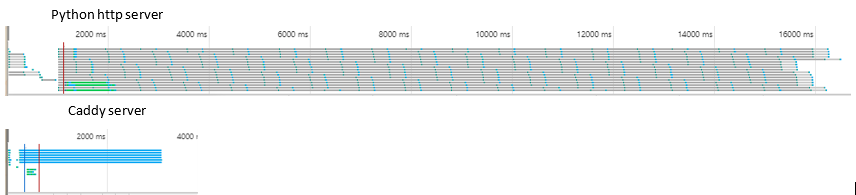
\includegraphics[width=.8\textwidth]{Pictures/CaddyVsPython}
	\caption{Screenshot of the network connection for a python and a caddy server}
	\label{CaddyVsPython}
\end{figure}


\fxnote{Mention caddy – 6 connection issue earlier}
 

\section{Not calculating minimum values in tiles} \label{WhyNoMin}

In the original version of the map both the minimum and maximum values were being calculated. However the program consistently defined the lowest value in currently visible tiles as 0.
This does not mean that all the tiles had minimum values of 0, just that there always were a tile in the map extent with a value of 0. In the vast majority of case the value would be 0. Few would be below 100. In the densest of cities the minimum value for some tiles was higher than 1000. 
It is possible that by zoom close enough to a major city it none of the tiles within view would have a value of 0 in which case the minimum value should be adjusted.
This is the main argument for calculating a minimum value. The downside of calculating it is that it has an significant effect on the processing time of the raster layer. Table \ref{tabMinimum} shows the time in seconds it takes for the layer to be rendered with and without calculating the minimum value. On average the rendering time is a second faster, when not calculating the minimum value.

\begin{table}[htbp]
	\centering
	\begin{tabular}{l}
		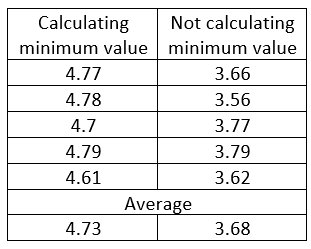
\includegraphics[width=0.4\textwidth]{Pictures/tabMinimum}
	\end{tabular}
	\caption{Seconds to fully render the website with and without calculating the minimum value}
	\label{tabMinimum}
\end{table}

The reason that the calculation of minimum value has such an effect on the processing time is presumably that the minimum value cannot be calculated in the same way as the maximum value. 
The maximum value is calculated by finding the maximum value in the array with all values. 
\fxnote{Write about nodata}
If the same operation is done to find the minimum value, the found minimum value often is -2147483648. As mentioned in section x that value means that no data is available for that pixel. 
It is therefore necessary to find the lowest positive value since no data is not the same as 0. This can be done by first filtering the raster, so only the positive values are left. The smallest of these values can then be calculated in the same way as the maximum value get calculated. 
It was decided that calculating a minimum value, which mostly would be 0 was not worth an additional second of loading. 

\chapter{Conclusion}
In this chapter the research questions listed below will be answered.
How can population rasters be visualized and compared efficiently and effectively?
Which conventions exist for visualization of population projections?
Which functionalities are relevant for comparing different rasters?
How can a responsive user experience be ensured, when loading and visualizing large raster dataset?


The intent with this project was to create a tool for easy visual comparison of raster datasets using population projections as a case. To create this, it was necessary to understand how raster data should be visualized and which functionalities a comparison tool should have.
How population raster should be visualized have been determined through a literature review of visualization conventions. 	
Population projections are based on quantitative data, which is ordered sequentially. While many visual conventions exist for the qualitative data, the same is not the case for quantitative data. A notable convention, which is relevant for quantitative data is that the “light is less dark is more”.
The functionalities needed for an interactive tool got selected by investigating a state-of-the-art interactive map. Based on this it was decided to add a search bar to enable easy navigation. 
To be able to compare different population projection two maps was displayed side by side. These were set up to always show the same area. The color of the projections inside was set up to automatically adjust to the population within the visible extent.
A lot of other features also present in the state-of-the-art map did not get implemented due to time constraints. 
To ensure a responsive user experience when visualizing large raster dataset technical requirements were set up for the solution. Some of which were important for the responsive user experience. The data loaded into the map should be limited to a minimum, since loading unnecessary data would slowdown or crash the tool. To limit the loaded data the population projection was divided into raster tiles. Only the tiles visible within the map’s extent would be loaded. These tiles were then colored based on the maximum and minimum values in the current extent. This meant that the same tile would be colored in different ways dependent on what was in the current extent. This coloring was done on the client instead of on the server.  This limited the number of requests to the server, since already loaded tiles could be reused. To be able to color the tiles at the client the tiles would contain information about population within each of their pixels instead of the pixels just having a color.
The responsiveness of the tool also got evaluated using the Lighthouse tool. Using this tool, it was discovered that the main factor for the responsiveness was the type of test server. Changing to Caddy as a test server reduced the tile loading time from 16 to below 4 seconds.
\fxnote{Maybe change technical concepts to technical requirements}


\fxnote{Write how it was accomplished from a technical perspective}
%Aside from the standard connected to the visualization of raster data there are also standard for the formatting of the raster files. Common raster formats include jpeg, png and tiff. One of the key differences between these formats are the bit depth. This value determines how many different colors that can be assigned each pixel in the image. Each bit can only be assigned one of two values, 0 or 1. This number of available colors for a pixel can therefore be calculated as $2^{number of bits}$. As an example, a bit depth of 8 bits would then result in $2^8 = 256$ different potential colors, since is the number of combinations of ones and zeroes, that are possible. For most maps this amount of colors is enough. The human eye can comprehend around 10 million different colors, but often that many colors are not needed. When displaying aerial photographs, the depth of 24 bits is often used, since it can display 16.7 million different colors and therefore can appear in true-colors to humans.
The limitations of the human eye does not mean that having more than 10 million bit combination is pointless. The bit combination can also be used for other thing than colors. It can be used to create transparency values or to store metadata about the image file. For instance, the geotiff format can use the additional bit to store georeferencing information.
These advantages of higher bit count come at a cost of a larger file size. Having a larger color depth will result in a slower loading and larger requirements for storage space.
Dent. 283 
\section{Tiled raster}
This section describes standards for dividing large raster files into smaller tiles. 
A way of only visualising the necessary parts of a raster is to divide it into smaller raster tiles and then only load the relevant tiles. When loaded into the map these tiles then gets places next to eachother, so they appear as a single large map image. These tiles can also be created with different resolutions, so that zooming in on the map with return tiles more details.  As illustrated in figure \ref{TilesPerZoomLevel} each of these zoom layers have more tiles.
 http://www.liedman.net/tiled-maps/
When zoomed all the way out the entire world is rendered as a single tile. Whenever the zoom level gets increased by one each tile in the previous layer get replaced with four smaller tiles. The number of tiles on a zoom level z can therefore be calculated as $2^2z$

$https://wiki.openstreetmap.org/wiki/Slippy_map_tilenames$
 

\begin{figure} [H]
	\centering
	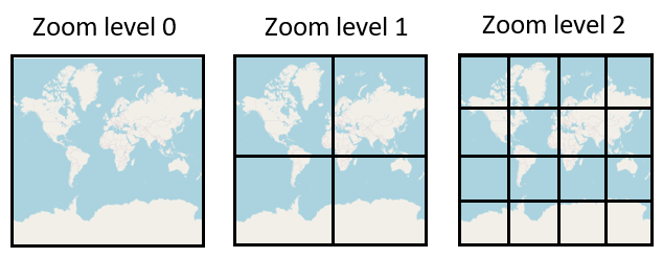
\includegraphics[width=.8\textwidth]{Pictures/TilesPerZoomLevel}
	\caption{Illustration of the increase in tiles for each zoom level}
	\label{TilesPerZoomLevel}
\end{figure}

Openstreetmaps is an example of a service, which use tiled rasters for their map. When this service is used, requests for tiles are send to 
http://tile.openstreetmap.org/zoom/x/y.png
In the request the values zoom, x and y are replaced with the current zoom level, tile column and tile row.
$https://wiki.openstreetmap.org/wiki/Slippy_map_tilenames$
 
 \begin{figure} [H]
 	\centering
 	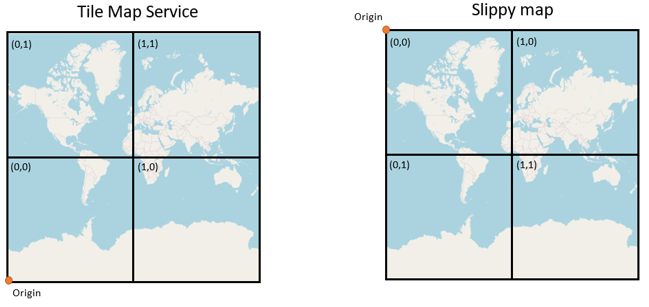
\includegraphics[width=.8\textwidth]{Pictures/TMSXYZ}
 	\caption{Illustration of the difference between the TMS and XYZ formats}
 	\label{TMSXYZ}
 \end{figure}
 
 %https://developers.planet.com/tutorials/slippy-maps-101/ https://wiki.osgeo.org/wiki/Tile_Map_Service_Specification#TileMap_Diagram 

The naming of these tiles are done differently for different standards. In this section only the Tile Map Service (TMS) and Slippy map (XYZ) standard will be addressed. Both of these have the same approach to naming zoom level and columns, but different approach to naming the rows. This difference has been illustrated in figure \ref{TMSXYZ}. The reason for the difference is that TMS tiles number their rows from south northwards, whereas XYZ are numbering rows the reverse way. Due to this difference in numbering rows loading tiles from the wrong standard results in a map as shown in figure \ref{SlippyInTMS}.
https://wiki.openstreetmap.org/wiki/TMS 
 
 
 \begin{figure} [H]
 	\centering
 	\includegraphics[width=.8\textwidth]{Pictures/SlippyInTMS}
 	\caption{How the map looks, when the TSM and XYZ get switched}
 	\label{SlippyInTMS}
 \end{figure}
 
\chapter{Initial research and related work}

Prior to developing the tool some initial experimentation with the case dataset was conducted. This lead to some core concepts which should apply to the developed tool. After this existing tool is described, which follows many of these core concepts.

\section{Core concepts}

Based on the initial research and tests a four core concepts were developed:
\begin{itemize}
 \item Load only the needed data
 \item Coloring should be based on the current extent
 \item Tiles should not be precolored
 \item Coloring should be done locally
 \item File format should have same bit depth as input format
\end{itemize}


\section{Load only the needed data}
The case data presented in chapter x holds information for the entire world. However, loading data for the entire world would be unnecessarily time consuming. Initial experiments of rendering this quantity of data also revealed that the browser did not have enough memory to load that amount of data. Instead only the relevant data should be downloaded. The relevant data in this case would refer to the data, which the user is able to see. Getting a subset of a raster dataset can be accomplished by dividing it into smaller tiles. Section x will present two different ways this can be achieved. 

\section{Coloring should be based on the current extent}
The initial exploration of the data showed that the coloring of the tiles should be based of the current extent. This is due to the how much the values are varying across the world. Figure \ref{WhyLimitToExtent} shows an example of the difference between a map where the coloring is based on all values or if it is limited to the current extent. Both maps illustrate the population in Denmark. The left map has its coloring based on values from the entire world, while the right has its colors based on the current extent. The left map appears empty since the population density in Denmark is negligible compared with the densest areas in the world. In the right map it is possible to see the location of the most populated cities. Since the left map provide the user with no relevant information and the right one does, the coloring should be based on the current extent.
 
 
\begin{figure} [H]
	\centering
	\includegraphics[width=.8\textwidth]{Pictures/WhyLimitToExtent}
	\caption{Population density in Jutland}
	\label{WhyLimitToExtent}
\end{figure}




\section{Tiles should not be precolored}
If the coloring should be based on the current extent and the map is interactive the coloring of the tiles should be done on the fly instead of once and for all. The reason for this is best explained with the example in figure \ref{WhyNotPrecolor}. This figure is illustrating the population in a small subset of India.  The three boxes are illustrating examples of possible map extents, which the user could get by zooming in on different parts of the map. Each of these three have a different max value in their cell with the highest population. The blue square is covering the city center of Indore a therefore have a high value than the green, which is covering the outskirts of the city. The last square does not include any part of a bigger city and therefore have a lower value. 
Since their max values are different, they would each need their own coloring. If the tiles were to be precolored it would be necessary, create three coloring of the tiles – one for each the extents. However, since the map is interactive, the extent is not limited to those three. If the user instead were to zoom in on an area between the red and blue square a new max value would maybe be found. When scaling this example up to the entire world and to multiple zoom extents there would be thousands of combinations. If all of these needed to be prerender it would both require lots of initial processing time and storage space for an immense amount of data. 
 
 
\begin{figure} [H]
	\centering
	\includegraphics[width=.8\textwidth]{Pictures/WhyNotPrecolor}
	\caption{Population density. The three boxes are examples of possible extents an interacting user could get by zooming.}
	\label{WhyNotPrecolor}
\end{figure}

The alternative is to color the tiles on the fly. When the user would zoom to a new area the map, a script could register the highest currently visible value. This information could then be sent to recoloring script, which would color the tiles based on this. This way only tiles with the needed colors would be rendered. 


\section{Coloring should be done locally}
The coloring can be done in two ways as illustrated in figure \ref{WhyColorLocally}. It can be done by sending the information to a tileserver, which then would color the tiles and send them to the client. Alternatively, the coloring could be done on the client. 
 
 \begin{figure} [H]
 	\centering
 	\includegraphics[width=.8\textwidth]{Pictures/WhyColorLocally}
 	\caption{Difference between coloring the tile on the server and locally}
 	\label{WhyColorLocally}
 \end{figure}
 
Comparing the two options is best done with an example, which has been illustrated in figure \ref{WhyColorLocallyMap}. Here the blue and green box are two different possible views both containing 16 raster tiles. The two boxes have different max values, since blue one contains the city center. In the example a user will pan from the blue view to the green one. If the coloring is done on the server side the initial 16 tiles in the blue box will be requested on load. Then when the user pan to the green view the 16 tiles in that box will be requested and colored. The four tiles that are shared between the blue and the green boxes must be requested again, since they need a new color due to the change in max value. This is not the case if the coloring is done locally. In this case only 12 tiles would have to be requested, when changing from the blue to the green view. Since the coloring is happening locally the coloring script can recolor the four tiles it already has downloaded from the initial load. This should result in a faster experience for the user.
   
\begin{figure} [H]
	\centering
	\includegraphics[width=.8\textwidth]{Pictures/WhyColorLocallyMap}
	\caption{Example of why local coloring is needed. The squares are different extents used for the example}
	\label{WhyColorLocallyMap}
\end{figure}

\section{File format should have same bit depth as input format}
As mention in section x the data from the case has a bit depth of 32 bit. To visualize the data the file format must not be changed to a format with less than 32 bits. Figure \ref{WhyColorLocallyMap} is an example of how a subset of the case data look originally and when converted to an 8-bit format. As mentioned in section x the pixels in an 8-bit raster can have values between 0-255. This means that this format is unable to correctly display the original data range, where the data range is covering thousands of values. The original data get clamped into the 8-bit format producing wrong result
https://gdal.org/programs/gdal2tiles.html .
 
 \begin{figure} [H]
 	\centering
 	\includegraphics[width=.8\textwidth]{Pictures/WhyColorLocallyMap}
 	\caption{32 bits cramped into 8 bits}
 	\label{WhyColorLocallyMap}
 \end{figure}
 
Normally this issue could be worked around by rescaling the input data to the new format https://gdal.org/programs/gdal2tiles.html . This rescaling would be a lossy compression resulting in loss of information since the original data cannot be expressed with values between 0-255. \citep{dent}
For the normal use of tiles this would not be a problem since tiles would only be used for visualization. 
If the tiles are being recolored locally the tiles are being used for more than just visualization. It is necessary to access the data within the tile. This means that solutions resulting in a lossy compression are not an option. To ensure that the correct data reach the client the file format used for tiles must have a bit depth of 32. 
  






\section{Related work}
This is not the first project to follow many of these core concepts. In Bernhard Baumrocks master thesis, he created a webmap, where raster tiles were being colored locally. \citep{Buamrocks}
\begin{figure} [H]
	\centering
	\includegraphics[width=.8\textwidth]{Pictures/BaumrockMap1}
	\caption{The map created by Bernhard Baumrock}
	\label{BaumrockMap1}
\end{figure}

A picture of one of his maps can be seen in figure \ref{BaumrockMap1}. This particular map is not included in his thesis, but it is the most similar to this project. The map shows an unspecified dataset colored in rainbow colors. Below the map are two sliders and a dropdown list with the label “rainbow”. Changing the value in this dropdown list allows the user to switch to another color scheme. The bottom slider is controlling the opacity for the raster layer. The upper slider controls which maximum and minimum values the coloring should be based on. How the map change, when changing the values in the upper slider can be seen in figure \ref{BaumrockMap2}. When zooming in another more detailed layer gets loaded and rendered.
\begin{figure} [H]
	\centering
	\includegraphics[width=.8\textwidth]{Pictures/BaumrockMap2}
	\caption{How the map change, when using the slider}
	\label{BaumrockMap2}
\end{figure}


%http://webportals.ipsl.jussieu.fr/ScientificApps/dev/forge_patrick/eox/map_01.html
 
When taking a closer look at the source code it can be seen that the raster is being loaded as tiff tiles with a bit depth of 16 bit. \citep{BuamrocksSouce} Only tiles the currently are visible are being requested unless the tile already have been requested. \citep{Buamrocks}

When comparing with the core concepts for this project, Baumrocks map fulfil most of the criteria. It is locally visualizing only the necessary data. The core concept related to bit depth is relevant in the creation of the tiles, so it does not really apply to this. 
It is also to some extent allowing the user to color the layer based on the current extent. The user can adjust the maximum and minimum values but does not know what the maximum values are in the current extent. 
How the tool functions from a technical perspective is further detailed in section x.

\section{Sections to be written here} 

Other ways of trying to visualizing large rasters:

\begin{itemize}
	\item qgis
	\item makeCitywebsite?
	\item Visualing with bokeh or folium 
\end{itemize}

Benchmarking using google lighthouse


\part{Development of the tool}
In this chapter it is explained how the tool has been developed. The first section is describing the coding languages used and the plugins used to create the tool. The following sections are describing the necessary steps to build the tool. These steps can be seen in figure \ref{DevelopmentSteps}.
 
 \begin{figure} [H]
 	\centering
 	\includegraphics[width=.8\textwidth]{Pictures/DevelopmentSteps}
 	\caption{An overview of the code}
 	\label{DevelopmentSteps}
 \end{figure}
 
First it is necessary to divide the raster into tiles to be able to limit the loaded data to the current extent. How this is done is explained in section x. Section x describes how the tiles have been visualized. To be able to color the tiles based on the current values it is required to know what the current values are. In section x it is explained how this information is calculated. The raster layer is then rerendered with these values as described in section x. Lastly some measurements were taken to ensure a more user-friendly experience. These additions are described in section x. 

\chapter{Coding languages and plugins}
For this project, the coding language Python was used to create the tiles, while visualization of the tiles was done in a webgis build with the languages HTML, CSS and Javascript. This webgis have been tested on a local caddy server for reasons explained in section x

\section{Languages}
\subsection*{Python}
Python is programming language with a simple syntax, which functions across multiple different platforms. This simple syntax means that Python can achieve the same as some other coding languages in fewer lines. $https://www.w3schools.com/python/python_intro.asp$
Python was used in this project because of the gdal library expanded further upon in section x
This project has been using version 3.6 of Python. 
\subsection*{HTML}
HTML is short for Hyper Text Markup Language. It is the language used for defining and structuring a web page’s content.
https://www.w3schools.com/js/default.asp
\subsection*{CSS}
CSS is an abbreviation for Cascading Style Sheets. This language defines how the HTML will be displayed.
\subsection*{Javascript}
How a webpage behaves is defined by the language Javascript.  This is what makes the web page interactive. 
\citep{CPL}

\section{Libraries}
To transform the raster data into smaller tiles the python library Gdal is used. 
\subsection*{Gdal}
GDAL is library for translating between multiple different geospatial data formats. https://gdal.org/ 

Included in this library is the gdal2tiles program, which can divide raster files into smaller tiles. 
At the time of using this program it was only able to generate tiles structured after the TMS standard. The function to follow the XYZ structure was added the 3th of May 2020 https://gdal.org/programs/gdal2tiles.html
%https://gdal.org/download.html#current-releases 
The script rendering the tiles in the map was based on the XYZ structure. This meant that the rows of tiles were ordered incorrectly when the generated tiles were imported. Therefore, the official version of gdal2tiles was replaced by a version made by a github user named commenthol. This version is modified to allow the creation of tiles following the XYZ structure. 
https://github.com/commenthol/gdal2tiles-leaflet
Both the official version and the modified version have their output format as mbtiles with a bit depth of 8 bit. To be usable for this project a bit depth of at least 32 bit is needed, as mentioned in section x. The workaround for this issue will be explained in section x. 
\subsection*{Openlayers}
The map in which the tiles are being showed are created in Openlayers, which is an open source JavaScript library for creating dynamic maps for web pages. 
https://openlayers.org/
Openlayers was chosen because the tool presented in related work was built in Openlayers. Therefore, using Openlayers would enable expanding upon this existing tool instead of starting from scratch. 

\subsection*{olGeoTiff}
olGeoTiff is a Javascript class for visualising geotiff tiles in Openlayers, utilising the libraries geotiff.js and Plotty. The visualized tiles are being processing in the client instead of on a server. It was used in the map presented in section x. 
The class is a modified version of Openlayers WMTS layer, where the internal tile loading function has been changed. The regular function would request precolored tiles and then add them to the map. The tiles requested by the modified version are not precolored and need to be processed before getting added to the map. A simplified illustration of this processing is illustrated in figure x. This simplified figure is enough to explain the mechanics of the class but does not detail the callback function structure. Aside from being used for error handling callbacks are also necessary to ensure that Openlayers do not try to add the tiles to the map, before they have been processed. More detailed figures can be found in Bernhard Baumrocks thesis.
 
 \begin{figure} [H]
 	\centering
 	\includegraphics[width=.8\textwidth]{Pictures/olGeoTiffSimplified}
 	\caption{A simplified illustration of how olGEoTiff functions}
 	\label{olGeoTiffSimplified}
 \end{figure}
 
To ensure that tiles are only being downloaded once an object keeps track of all the downloaded data. The object is organized by the tiles’ url. 
Whenever tiles are being requested the object will always be checked to see if it already contains the url. If it does not the object will be updated to include the requested tile. The tile will then be loaded before being processed. 
The processing is done with the TIFF parser geotiff.js 
https://geotiffjs.github.io/
and Plotty, which is a library for creating images from data arrays.
https://github.com/santilland/plotty
. The loaded tiles first get parsed with geotiff.js and added to the object before Plotty get used to render tiles in the designated colors. Then the tiles get added to the map.
\citep{BThesis}
https://web.archive.org/web/20191031034339/https://eox.at/2018/01/visualizing-geotiff-tiles-with-openlayers/
The olGeoTiff also have a redraw function, which when triggered will redraw the tile layer based on the current designated colors. This was for instance used in Bernnard Baumrocks map, whenever the color sliders were changed. 

%\section{Testserver}
%Not finished
%The solution was being tested in Google Chrome initially using a python-based http server. This was later replaced with a Caddy server to improve performance. 
% 
%Caddy
%http’s limits to 6 connections 
%fig text: Blue: DomContentLoaded Red: Load

\chapter{Developing the tool}
This chapter details how the visualization tool was built.

\section{Creating the tiles}
The tiles got created using a modified version of gdal2tiles, which was changed to create tiles following the XYZ format. However, since the default output bit depth is too low, it would have to be modified further. The file format would also have to be changed to tiff in order to be visualized with the geotiff.js library. 

\subsection{Changing the file type}
Changing the file format can be done by changing two lines in the gdal2tiles script:

\begin{lstlisting}[language=iPython, caption={Changing the file format}, label= VoresPY,escapechar=|]
 #Original code
#self.tiledriver = 'PNG'
#self.tileext = 'png'
#New code
self.tiledriver = 'GTiff'
self.tileext = 'tiff'
\end{lstlisting}
This changes the raster driver from png to the geotiff format and the file extension from png to tiff. 
https://gdal.org/drivers/raster/index.html
The geospatial information, which is the difference between a geotiff and a regular tiff, gets lost in process. This information is not important for this project since the tiles are being loaded based on their name and folder placement, not based on the internal metadata.

Running gdal2tiles with these changes will produce a tiff file, which still would be limited to 8 bits. 
\subsection{Increasing the bit depth}
The reason for the bit limit is that gdal2tiles uses the memory dataset driver, which have 8 bits as default.  This default can overwritten to 32 bits by adding “gdal.GDT\_Int32” to every instance where the driver is being used as demonstrated in code x. 
http://osgeo-org.1560.x6.nabble.com/gdal-dev-gdal2tiles-for-16bit-data-tp5163094p5163098.html

\begin{lstlisting}[language=iPython, caption={Increasing the bit depth}, label= VoresPY,escapechar=|]
self.mem_drv = gdal.GetDriverByName('MEM')
...
#Old code
#dstile = mem_drv.Create('', tile_size, tile_size, tilebands)
#New code
dstile = self.mem_drv.Create('', self.tilesize, self.tilesize, tilebands, gdal.GDT_Int32)
\end{lstlisting}
The memory driver is being used four times, which all have been changed in a similar fashion.

Running the script with these changes produces tiles with the correct format and bit depth. The script also produces an xml file with metadata. An example of the content of said metadata file can be seen in code x.

\begin{lstlisting}[language=HTML5, caption={The metadata from the xml file generated by the modified gdal2tiles}, label= VoresHTML,escapechar=|]
<?xml version="1.0" encoding="UTF-8"?>
<TileMap tilemapservice="http://tms.osgeo.org/1.0.0" version="1.0.0"><Abstract/><SRS>GEOGCS["WGS 84",DATUM["WGS_1984",SPHEROID["WGS 84",6378137,298.257223563,AUTHORITY["EPSG","7030"]],
AUTHORITY["EPSG","6326"]],PRIMEM["Greenwich",0,AUTHORITY["EPSG","8901"]],UNIT["degree",0.0174532925199433,
AUTHORITY["EPSG","9122"]],AXIS["Latitude",NORTH],AXIS["Longitude",EAST],AUTHORITY["EPSG","4326"]]
</SRS><BoundingBox maxy="25.00000000000814" maxx="80.99999999999989" miny="19.00000000000815" minx="72.99999999999989"/><Origin y="19.00000000000815" x="72.99999999999989"/><TileFormat extension="tiff" mime-type="image/tiff" height="256" width="256"/><TileSets profile="raster"><TileSet order="2" units-per-pixel="0.00833333333333" href="2"/><TileSet order="3" units-per-pixel="0.00416666666667" href="3"/><TileSet order="4" units-per-pixel="0.00208333333333" href="4"/><TileSet order="5" units-per-pixel="0.00104166666667" href="5"/><TileSet order="6" units-per-pixel="0.00052083333333" href="6"/><TileSet order="7" units-per-pixel="0.00026041666667" href="7"/><TileSet order="8" units-per-pixel="0.00013020833333" href="8"/><TileSet order="9" units-per-pixel="0.00006510416667" href="9"/></TileSets></TileMap>
\end{lstlisting}


How long time did it take to run?

Running it parallelly it parallelly 

\section{Visualizing tiles}
After the tiles got created, they are stored in a folder, which gets uploaded to the testserver along the index file. 
The metadata from the xml file must be loaded into the map to be able to visualize the tiles. Normally this could be done using the WMTSCapabilities() function in Openlayers.
https://openlayers.org/en/latest/examples/wmts-layer-from-capabilities.html 
However, the formatting of the xml file produced by gdal is different from the format, which this function can read. Therefore, a small script has been created to parse the xml file and store the information in a metadata object. This object, tileMetadata, stores the bounding box, origin, center coordinates as well as tilesize. The initial version of the object also stored the resolution data, which is called units-per-pixel in code x. This led to some inconsistency when loading tiles, which had been generated without some of the lower zoom level. This will be further expanded upon in section x. Therefore, the resolution was instead generated using the script x, where 0.0333 is the value for units-per-pixel at zoom level 0. 

\begin{lstlisting}[language=JavaScript, caption={The JavaScript in the project}, label= VoresJS,escapechar=|]
for (var z = 0; z < 14; ++z) {
  // generate resolutions and matrixIds arrays for this WMTS
  //The number in the resolution calculation is the units-per-pixel value at zoomlayer 0 in the xml file generated by gdal2tiles
  resolutions[z] = 0.03333333333514 / Math.pow(2, z);
  matrixIds[z] = z;
}
\end{lstlisting}
Using this metadata, the tiles could be visualized using the olGeoTiff class. 

%\begin{lstlisting}[language=JavaScript, caption={The JavaScript in the project}, label= VoresJS,escapechar=|]
%var wmslayer = new ol.layer.Tile({
%  source: new ol.source.WMTS({
%    url: tileFolders + '/{TileMatrix}/{TileCol}/{TileRow}.tiff',
%    projection: projection,
%    tileGrid: new ol.tilegrid.WMTS({
%      origin: tileMetadata[origin],
%      resolutions: resolutions,
%      matrixIds: matrixIds,
%      tileSize: tileMetadata[tileSize],
%    }),
%    requestEncoding: 'REST',
%    transition: 0
%  }),
%  extent: tileMetadata[boundingBox],
%  opacity: 0.65 
%});
%var olgt_map = new olGeoTiff(wmslayer);
%\end{lstlisting}


\subsection{Custom colors scheme}
Using colorbrewer a custom sequential colorscheme was generated. This scheme was added to Plotty and selected as a color palette.
*This code might change a bit, so wait with writing  


\section{Loading data at a wrong resolution}
Figure x shows how the map looked, when loaded with a manually defined max value.
 
 
 \begin{figure} [H]
 	\centering
 	\includegraphics[width=.8\textwidth]{Pictures/MapWithWrongResolution}
 	\caption{The map looking right, but with tiles from the wrong zoom level}
 	\label{MapWithWrongResolution}
 \end{figure}


While the map appeared to look alright, it was loading tiles from the wrong zoom level. The tiles always got loaded from a zoom level 3 lower than intended. So the map in figure x is visualizing the map at zoom level 7 but loading and displaying tiles from zoom level 4.

Some experiments with loading the tiles from the correct zoom level 
Setting up Openlayers to download tile from the current view and correct zoom level chrashed the map with the error message “Insufficient Resources”. The amount of loaded tiles seems unnecessarily high and size of the tiles too small. This seems to indicate, that the tiles, which the modified version of gdal2tiles associates with zoom level 7 in fact belongs to a higher zoom level.

The reason for this bug was never discovered and the bug never got fixed. When the resolution data was gathered from the metadata file, the difference between the loaded and the actual zoom level would between different sets of tiles. This variance would depend on the which zoom levels were not being generated. So, if only the zoom levels 2-7 were generated, the difference would increase by one for each missing layer. In this case the loaded tiles would instead be wrong by 5, calculated as the default wrongness of 3 plus 2 for missing zoom layer 0 and 1. 
This bug will be defining for the rest of the code.



\section{Calculate max value in current extent}
Calculating the highest value in the current extent can be divided into two smaller tasks. Figuring out which tiles currently are being displayed and processing these tiles.

\subsection{Current displayed tiles}

The tiles, which currently is within the view, can be found using the Openlayers tileGrid method forEachTileCoord. This method can trigger a function for each tile within a given zoom level and extent. 
%https://openlayers.org/en/latest/apidoc/module-ol_tilegrid_TileGrid-TileGrid.html#forEachTileCoord
The method is going through the tiles based on their coordinates, but this can be translated to the tile urls using the getTileUrlFunction.
var tileUrlFunction = wmslayer.getSource().getTileUrlFunction()
var zoomlevelAdjustment = 3
wmslayer.getSource().getTileGrid().forEachTileCoord(loadExtent, mapZoom - zoomlevelAdjustment, function(tileCoord) {
tileName = tileUrlFunction(tileCoord, ol.proj.get('EPSG:4326'))
%Find max value
}
forEachTileCoord is triggering for each tile in the given zoom extent. This means that it on zoom level 7 it would load the tiles, that should be rendered on zoom level 7. Due to the bug mentioned section x it is not the tiles from that zoom level, which are being displayed. Instead the tiles from zoom level 2 are being displayed. This will complicate some of the next steps. 
The adjustment to the zoom level is in order to load the tiles, which should have displayed.

\subsection{Max value for each tile}
If the tiles added to the map had been from the correct zoom level calculating max value of a tile could have been done as olGeoTiff were running. olGeoTiff holds the values for the tiles in a dataarray already, so finding the maximum value could be done with a single line adding a tiles max value to the dictionary for that tile. This line is shown in code x, where urlToTiff is the name of the object, which holds the data.
        maxValueTileData[url].maxValue = Math.max(...urlToTiff[url][0])
However, since olGeoTiff holds data from an incorrect zoom layer this would not function. A possible solution would be to trigger forEachTileCoord for the same wrong zoom layer as the displayed tiles are from. This solution was not implemented since it would result in a map with could potentially so misleading information. The explanation for this has been illustrated in figure x. 

Todo: Figure with showing how large the loaded tiles are compared with how large they should be.

The tiles from the wrong zoom level are so large, that they would show data outside the view of the map. This means that the coloring could be based on the information that was outside of the current view.

The alternative solution is to run another function going through the tiles, which should have been displayed and find the highest value among these. This would result in a map where the wrong tiles were being colored based on information from the smaller correct tiles. This solution is by no means ideal. It means requesting tiles from two layers, one for displaying on the map a one for calculating the relevant max values. Loading more data than necessary will make the script slower, but since no better solution was not found this have been implemented.
The calculation of the maximum value for each tile was done in a very similar fashion to how olGeoTiff operates as illustrated in figure \ref{CalculateMaxValue}. An object holds information about all tiles, which have been processed and the max value is known. When the function is run for a tile it first checks if the tile already has been processed. If that is not the case, then it will create an object for the data, which it then will load and parse with geotiff.js. The data array with parsed data will then be run through as descripted in code x to calculate the maximum value. This maximum value will then be returned to the map. 

 
\begin{figure} [H]
	\centering
	\includegraphics[width=.8\textwidth]{Pictures/CalculateMaxValue}
	\caption{Flow diagram of the calculation over max value in a tile}
	\label{CalculateMaxValue}
\end{figure}



\subsection{Highest tile value the current displayed}


To find the largest tile value among all the currently displayed tiles forEachTileCoord as mentioned earlier is used. forEachTileCoord does not have a trigger for when it has run through all the tiles. This functionality is necessary for ensuring that the produced maximum value is actually the maximum value. Without a precise end trigger the coloring applied to the map could be based on the biggest value found before the coloring script stated running instead of the absolute highest value in the current display.
Since this trigger is necessary it has been created by running forEachTileCoord another time to count the number of tiles. This part of the code can be seen in code x. 
  var tileNumber = 0;
  wmslayerMap1.getSource().getTileGrid().forEachTileCoord(loadExtent, mapZoom - zoomlevelAdjustment, function(tileCoord) {
    tileNumber++;
  })
The total number of tiles in the current extent can then be used as a trigger. 
The recoloring of the map can then be delayed until the function for calculating the maximum value have been running for the same amount of times as there are tiles on the map. In practical terms this can be accomplished by adding a counter and an if statement to the maximum-value-function. The counter would check how many times the function has run. The if statement would check if the amount of time the function had been run was equal to the number of tiles. If this is the case and the registered max value is different from the previous one the recolor function would trigger.
The calculation of the maximum value is the function presented in figure \ref{DoubleLoop}. It is running asynchronously because the array otherwise would be filled with “undefined” values instead of actual values. Running it asynchronously ensures that the script awaits the calculation of the value.  
 \begin{figure} [H]
 	\centering
 	\includegraphics[width=.8\textwidth]{Pictures/DoubleLoop}
 	\caption{Finding the largest value in all currently displayed tiles}
 	\label{DoubleLoop}
 \end{figure}

\section{Recolor when the max value change}

The recoloring function was already part of olGeoTiff. However, in Bernhard Baumrocks’ thesis this recoloring was triggered manually by the user when changing the color sliders. In this project the changing of colors will trigger automatically. The function for recoloring the map have therefore been set up to trigger on the user stopping this changing the view. By not triggering before the map movement is finished a smoother user experience is ensured, since new tiles does not have to processed before the user is finished with interacting with the map. The recolor function is running through all of the code mentioned in the previous sections. 

\begin{lstlisting}[language=JavaScript, caption={The JavaScript in the project}, label= VoresJS,escapechar=|]
  map.on("moveend", function() {
    recolorMap()
  });
});
\end{lstlisting}
\section{Polish}
In addition to the rendering of the raster in the map, some features were also added to improve the user experience.


\subsection{Two maps}

\begin{figure} [H]
	\centering
	\includegraphics[width=.8\textwidth]{Pictures/DualMaps}
	\caption{A second map}
	\label{DualMaps}
\end{figure}
To be able to compare different rasters with eachother a second map was added as illustrated in figure \ref{DualMaps}. This second map is having its own raster dataset but sharing the view with the first map. This means that the two maps would always show the same area. Panning or zooming in one map would do the same action in the other map. The two maps are sharing the same legend. 
 

%Add to dualmaps how the double evaluation for multiple maps were build 

\subsection{Search function}
In order to be able to faster navigate the map a search function was created as shown in figure \ref{SearchBar}. 
 
 \begin{figure} [H]
 	\centering
 	\includegraphics[width=.8\textwidth]{Pictures/SearchBar}
 	\caption{A searchbar}
 	\label{SearchBar}
 \end{figure}
 
The user can use this to change the current view of the maps to a given location. This is accomplished through the help of Nominatim. This tool can search through Openstreetmap data by location names. It then returns data about the searched location. 
https://wiki.openstreetmap.org/wiki/Nominatim

Among this data is the latitude and longitude for the central point of the place.    
%https://nominatim.openstreetmap.org/details.php?osmtype=N&osmid=245709027&class=place
This coordinate is then used as the coordinate for the center of the map.


% \section{Tabulars}

\subsection{Real tabulars}

here are some text

\begin{table}[h]%You have to add this h yourself
\centering
\begin{tabular}{|c|cc|}
\hline
\multicolumn{2}{|c|}{Item}                   & \multicolumn{1}{r|}{} \\ \hline
Animal    & \multicolumn{1}{c|}{Description} & Price (\$)            \\ \hline
Gnat      & \multicolumn{1}{c|}{Frozen}      & 13.65                 \\ \hline
Gnu       & \multicolumn{1}{c|}{Stuffed}     & 92.50                 \\ \hline
Emu       & \multicolumn{1}{c|}{Stuffed}     & 33.33                 \\ \hline
Armadillo & \multicolumn{1}{c|}{Frozen}      & 8.99                  \\ \hline
\end{tabular}
\caption{This a real tabular}
\label{my-label}
\end{table}

also here

\subsection{Fake tabulars}



\begin{table}[htbp]
  \centering
    \begin{tabular}{l}
    \includegraphics[width=0.5\textwidth]{Pictures/Tab}
    \end{tabular}%
  \caption{Add caption}
  \label{tab:addlabel}%
\end{table}%




%%%% Kilder %%%%

\begingroup
	\raggedright
	\bibliography{bibtex/litteratur}
	\endgroup	  % Litteraturlisten inkluderes



%%%% Appendiks %%%%

\appendix														% Appendiks/bilag start - giver chapter bogstaver i stedet for tal
\clearforchapter												% Sikrer at pagestylen aktiveres paa den rigtige side
\phantomsection													% Kunstigt afsnit, som hyperlinks kan 'holde fast i'
\pdfbookmark[0]{Appendiks}{appendiks}							% Tildeler en klikbar bookmark til den endelige PDF


% Indstillinger for appendiks (deaktiveret med "%") %%

\pagestyle{empty}												% Sidehoved/-fod for standardsider aendres til tom for appendiks
\aliaspagestyle{chapter}{empty}								% Sidehoved/-fod for kapitelsider aendres til tom for appendiks
\settocdepth{chapter}											% Kun kapitel-niveau vises i ToC
%\addtocontents{toc}{\protect\cftpagenumbersoff{chapter}}		% Sidetal for kapitler fjernes i ToC

% Filer til appendiks %%

\chapter{Lighthouse audit}\label{Audit}


\includegraphics[width=1.2\textwidth, angle=90]{Pictures/Audit1}

\includegraphics[width=1.2\textwidth, angle=90]{Pictures/Audit2}

\includegraphics[width=0.6\textwidth, angle=90]{Pictures/Audit3}
\chapter{The code in the project}


\section{HTML and CSS}

\begin{lstlisting}[language=HTML5, caption={The HTML and CSS in the project}, label= VoresHTML,escapechar=|]

<!DOCTYPE html>
<html>

<head>
<meta charset="utf-8" />
<link rel="shortcut icon" href="#" />
<title>maps from geotiff</title>

<script src="./lib/jquery.min.js"></script>

<script src="./lib/plotty.min.js"></script>
<script src="./lib/geotiff.browserify.js"></script>

<script src="./lib/olGeoTiff.js"></script>
<script src="./lib/ol-debug.js"></script>
<link rel="stylesheet" href="./lib/ol-debug.css">
<link rel="stylesheet" href="https://cdnjs.cloudflare.com/ajax/libs/font-awesome/4.7.0/css/font-awesome.min.css">

<style>
body {
font-family: Arial, sans-serif;
font-size: 14px;
}

.map {
width: 400px;
height: 400px;
margin-top: 20px;
}

.mapcontainer {
padding: 0 100px;
text-align: center;
}

td {
border: 0;
margin: 0
}

td.l {
color: white;
text-align: center;
width: 30px;
height: 30px;
padding: 0
}

@media (min-width: 900px) {
.wrapper {
display: flex;
}

.half {
padding: 0 10px;
width: 400px;
float: left;
}
}
</style>
</head>

<body>
<input type="text" id="requestedCity" value="Search">
<button onclick="SearchCity()"><i class="fa fa-search"></i></button>
<div class="wrapper">
<div class="half">
<h4 id="firstMapName">Map1</h4>
<div id="firstmap" class="map"></div>
</div>
<div class="half">
<h4 id="secondMapName">Map2</h4>
<div id="secondMap" class="map"></div>
</div>
</div>
<!-- Add legend -->
<table>
<tr>
<td colspan="6">Population per cell</td>
</tr>
<tr>
<td class='l' id='d0' title='0'></td>
<td class='l' id='d1' title='0'></td>
<td class='l' id='d2' title='0'></td>
<td class='l' id='d3' title='0'></td>
<td class='l' id='d4' title='0'></td>
<td class='l' id='d5' title='0'></td>
</tr>
<tr>
<td colspan="4" style='text-align: left'>0</td>
<td></td>
<td id="MaxValue" colspan="4" style='text-align: right'>0</td>
</tr>
</table>

<script src="tileMetadata.js"></script>
<script src="map.js"></script>

</body>

</html>

\end{lstlisting}


\section{Javascript}
\begin{lstlisting}[language=JavaScript, caption={The JavaScript for the map}, label= VoresJS,escapechar=|]

////////////
// Getting Metadata
////////////



//The folder, where the tiles are extracted from.
var tileFolders = ['g2tTiles', 'g2tSecondMap']

//Add layer names to map
document.getElementById('firstMapName').innerHTML = tileFolders[0]
document.getElementById('secondMapName').innerHTML = tileFolders[1]
//Get tile-metadata produced by gdal2tiles32 and store it in the tileMetadata object.
var tileMetadata = {};
getTileMetadata(tileMetadata, tileFolders);

//Resolutions from the metadata xmlfile creates issues with loading the correct file if any zoomlayers are excluded
//Therefore resolutions tables are created manually.
var resolutions = new Array(14);
var matrixIds = new Array(14);
for (var z = 0; z < 14; ++z) {
// generate resolutions and matrixIds arrays for this WMTS
//The number in the resolution calculation is the units-per-pixel value at zoomlayer 0 in the xml file generated by gdal2tiles
resolutions[z] = 0.03333333333514 / Math.pow(2, z);
matrixIds[z] = z;
}

////////////
// Creation of colorscale
////////////

//Here a color scale is created and added to the available color scales
//The colors are selected in colorbrewer - https://colorbrewer2.org/#type=sequential&scheme=OrRd&n=6
var colorScale = {};
colorScale.color_steps = [
'#fef0d9',
'#fdd49e',
'#fdbb84',
'#fc8d59',
'#e34a33',
'#b30000'
]
colorScale.percentage_steps = [
0,
0.2,
0.4,
0.6,
0.8,
1
]
plotty.addColorScale("sequentialMultiHue6Colors", colorScale.color_steps, colorScale.percentage_steps);

////////////
// Creating the map
////////////

// Setting map projection
const projection = new ol.proj.get('EPSG:4326');

//Create the layers with the raster tiles. Some metadata is collected from the metadta object
var wmslayerMap1 = new ol.layer.Tile({
source: new ol.source.WMTS({
url: tileFolders[0] + '/{TileMatrix}/{TileCol}/{TileRow}.tiff',
projection: projection,
tileGrid: new ol.tilegrid.WMTS({
origin: tileMetadata[tileFolders[0] + "origin"],
resolutions: resolutions,
matrixIds: matrixIds,
tileSize: 256
}),
requestEncoding: 'REST',
transition: 0
}),
//The extent has been limited, since there I didn't test with the raster for the entire world
extent: tileMetadata[tileFolders[0] + "boundingBox"],
opacity: 0.65
});

var wmslayerMap2 = new ol.layer.Tile({
source: new ol.source.WMTS({
url: tileFolders[1] + '/{TileMatrix}/{TileCol}/{TileRow}.tiff',
projection: projection,
tileGrid: new ol.tilegrid.WMTS({
origin: tileMetadata[tileFolders[1] + "origin"],
resolutions: resolutions,
matrixIds: matrixIds,
tileSize: 256
}),
requestEncoding: 'REST',
transition: 0
}),
extent: tileMetadata[tileFolders[1] + "boundingBox"],
opacity: 0.65
});

// define the base layer
var osmSource = new ol.source.OSM();
var osm = new ol.layer.Tile({
source: osmSource
});

// This view is shared between both maps, so they always show the same
var sharedView = new ol.View({
projection,
center: tileMetadata[tileFolders[0] + "center"],
zoom: 7,
maxZoom: 11,
minZoom: 2
})

// define the left map
var map = new ol.Map({
target: 'firstmap',
layers: [
osm, wmslayerMap1
],
wrapDateLine: true,
view: sharedView
});

// define the right map
var map2 = new ol.Map({
target: 'secondMap',
layers: [
osm, wmslayerMap2
],
wrapDateLine: true,
view: sharedView
});



// olGeoTiff setup
var olgt_map1 = new olGeoTiff(wmslayerMap1);
var olgt_map2 = new olGeoTiff(wmslayerMap2);
olgt_map1.plotOptions.palette = 'sequentialMultiHue6Colors';
olgt_map2.plotOptions.palette = 'sequentialMultiHue6Colors';

// Color the maps based on their values
recolorMap()
// handle user input
$(window).on('load', function() {

//Add the colors from the color palette to the legend
for (i = 0; i < colorScale.percentage_steps.length; i++) {
document.getElementById('d' + String(i)).style.background = colorScale.color_steps[i]
}

//Recolor map on movement or zoom
map.on("moveend", function() {
recolorMap()
});

});

////////////
// Recoloring the map
////////////
// Find the highest value currently displayed and recolor based on this

//variable for holding the max value and checking if the max value changes
var currentMax = 0;
var oldMax = currentMax;

function recolorMap() {

//Array holding max values for all currently displayed tiles
var maxValuesAllTiles = [];

//Getting map extent and zoom
var mapExtent = map.getView().calculateExtent(map.getSize())
var mapZoom = map.getView().getZoom();

//This variable is adjusting for the fact that the wrong zoom level is being loaded
var zoomlevelAdjustment = 3

//The loadExtent is the same as the mapextent, unless the mapextent shows an area outside the data area
// In this case the loadExtent gets reduced to the bounding box -
// this is to avoid attempt at loading data, which doesn't exist
var loadExtent = new Array(4);
loadExtent[0] = Math.max(mapExtent[0], tileMetadata[tileFolders[0] + "boundingBox"][0]);
loadExtent[1] = Math.max(mapExtent[1], tileMetadata[tileFolders[0] + "boundingBox"][1])
loadExtent[2] = Math.min(mapExtent[2], tileMetadata[tileFolders[0] + "boundingBox"][2])
loadExtent[3] = Math.min(mapExtent[3], tileMetadata[tileFolders[0] + "boundingBox"][3])

//Get the total number of tiles - both maps have the same number of tiles, so no need to run this twice
var tileNumber = 0;
wmslayerMap1.getSource().getTileGrid().forEachTileCoord(loadExtent, mapZoom - zoomlevelAdjustment, function(tileCoord) {
tileNumber++;
})

//Counting variables keeping track of how many tiles have been processed in each map
var currentTile = {};
currentTile[tileFolders[0]] = 0;
currentTile[tileFolders[1]] = 0;

//Calculate the highest value in each map. The counting variables have been included to know when to draw the layer
findHighestValue(wmslayerMap2, tileFolders[1], tileFolders[0])
findHighestValue(wmslayerMap1, tileFolders[0], tileFolders[1])

function findHighestValue(wmslayer, selfCounter, otherCounter) {

//Getting the url (name) of the tile based on its coordinates
var tileUrlFunction = wmslayer.getSource().getTileUrlFunction()

//Checks which tiles that currently are being displayed
//This is done at a lower resolution than the current zoomlevel, since loading otherwise would be too slow
wmslayer.getSource().getTileGrid().forEachTileCoord(loadExtent, mapZoom - zoomlevelAdjustment, function(tileCoord) {

//Gets the name of each currently displayed tile
tileName = tileUrlFunction(tileCoord, ol.proj.get('EPSG:4326'))
asyncCall()
async function asyncCall() {

//Get the maximum value in the tile and add it to the array
tileMaxValue = await calculateMaxValue(tileName);
maxValuesAllTiles.push(tileMaxValue)
//Update the counter - one more tile have been processed
currentTile[selfCounter]++;

//Checks if the function is finished with finding max value for tiles in both layers
if (currentTile[selfCounter] == tileNumber && currentTile[otherCounter] == tileNumber && tileNumber != 0) {

//Resets all counters and set current max to the highest value
currentTile[selfCounter] = 0;
currentTile[otherCounter] = 0;
tileNumber = 0;
currentMax = Math.max(...maxValuesAllTiles)
//Recolor the map, if max value have changed
if (Number.isInteger(currentMax) && currentMax != oldMax) {
oldMax = currentMax
olgt_map1.redraw(olgt_map1, currentMax, colorScale);
olgt_map2.redraw(olgt_map2, currentMax, colorScale);
}
}

}
})

}

}



//This function pans to a searched city.
function SearchCity() {
//Get the name from the search bar and request the coordinates for it from Nominatim
var cityName = document.getElementById("requestedCity").value;
var request = "https://nominatim.openstreetmap.org/search?q=" + cityName + "&format=geojson"

var xhttp = new XMLHttpRequest();

xhttp.onreadystatechange = function() {
if (this.readyState == 4 && this.status == 200) {
var cityData = JSON.parse(this.responseText)
var cityCoordinates = cityData.features[0].geometry.coordinates

map.getView().setCenter(cityCoordinates)
map.getView().setZoom(9)

}
}
xhttp.open("GET", request, true);
xhttp.send();

}

\end{lstlisting}

\begin{lstlisting}[language=JavaScript, caption={The JavaScript for getting Metadata about tiles}, label= VoresJS,escapechar=|]
//Making a request for the tileData - see function getTileMetadata
function getTileMetadata(objectWithMetadata, folderArray) {
for (i = 0; i < folderArray.length; i++)
{

var xhttp = new XMLHttpRequest();
xhttp.open("GET", folderArray[i] + "/tilemapresource.xml", false);
xhttp.send();
processTileMetadata(xhttp, objectWithMetadata, folderArray[i]);

}
}

//When gdal2tiles32.py is run it creates a xml file with metadata. This function extracts the relevant data
function processTileMetadata(xml, objectWithMetadata, folderName) {
var xmlDoc = xml.responseXML;
var parser = new DOMParser();
var xmlDoc = parser.parseFromString(xml.responseText, "application/xml");

//Getting the coordinates for bounding box, origin and center
var minx = parseFloat(xmlDoc.getElementsByTagName("BoundingBox")[0].attributes.minx.value);
var maxx = parseFloat(xmlDoc.getElementsByTagName("BoundingBox")[0].attributes.maxx.value);
var miny = parseFloat(xmlDoc.getElementsByTagName("BoundingBox")[0].attributes.miny.value);
var maxy = parseFloat(xmlDoc.getElementsByTagName("BoundingBox")[0].attributes.maxy.value);
objectWithMetadata[folderName + "boundingBox"] = [minx, miny, maxx, maxy]
objectWithMetadata[folderName + "origin"] = [minx, maxy]
objectWithMetadata[folderName + "center"] = [
(minx + maxx) / 2,
(miny + maxy) / 2
]

}
\end{lstlisting}


\begin{lstlisting}[language=JavaScript, caption={Additions to olGeoTiff.js. The original code can be found at \citet{olGeoTiffSource}}, label= VoresJS,escapechar=|]

//Everything above is the same as the original olGeoTiff file

olGeoTiff.prototype.redraw = function(map, currentMax, legendValues) {

map.plotOptions.domain = [0, currentMax];
this.layer.getSource().refresh();
updateLegend(legendValues, currentMax);
}


// Updates the legend
function updateLegend(colorValues, maxValue) {
//Updates the number displaying the maximum value
document.getElementById('MaxValue').innerHTML = maxValue;
//Updates the values shown, when holding the mouse over the individual color classes
for (i = 0; i < colorValues.percentage_steps.length; i++) {
document.getElementById('d' + String(i)).title = Math.round(colorValues.percentage_steps[i] * maxValue)
}
}

// This object contains the maximum value for the loaded tiles data
var maxValueTileData = {};

//Returns the maximum value for a given tile. In the value does not exist it will be calculated and added to the object
function calculateMaxValue(url) {
//The value gets returned as a asynchronous function, since it otherwise would return undefined
return new Promise(resolve => {

//If the tiles have previously been loaded and stored in the object, then it is returned
if (maxValueTileData[url]) {
resolve(maxValueTileData[url].maxValue)
}
//If the tile is not in the object, then it gets calculated, added to the object and then returned
else {
maxValueTileData[url] = {
maxValue: 0 //Edited
};

// send new request
var xhr = new XMLHttpRequest();
xhr.open('GET', url, true);
xhr.responseType = 'arraybuffer';

// setup the async function that is executed AFTER the tile was loaded
xhr.onloadend = function(e) {
if (xhr.status == 200) {
// save rasters of parsed tiff
var parsed = GeoTIFF.parse(this.response);
var raster = parsed.getImage().readRasters();
// calculate the maximum value in the tile
var maxPop = Math.max(...raster[0])

//Add to the object and return the value
maxValueTileData[url].maxValue = maxPop
resolve(maxValueTileData[url].maxValue)
}
//
//       // send ajax request
}
xhr.send();

}

})
}
\end{lstlisting}




%\includepdf[pages={1-3}]{Appendix/LighthouseAudit.pdf}



%Flyt nederst

%%%% Bilag %%%%

%\phantomsection												% Kunstigt afsnit, som hyperlinks kan 'holde fast i'
%\addcontentsline{toc}{chapter}{Bilag A \ Navn} 				% Manuelle indgange i indholdsfortegnelsen (naar \includepdf bruges)
%\cleardoublepage
% Inkluder eksterne bilag med \includepdf[pages={x-y}]{filnavn}


%%%% Fixme-listen %%%%

\newpage														% Ny side til Fixme-listen
\listoffixmes													% Fixme-listen - fjernes til sidst i projektet med "%"



\end{document}													% % Slutter dokumentet - obligatorisk